\documentclass[a4paper]{article}

% Use the postscript times font!
\usepackage{times}
\usepackage{soul, color}
\usepackage[hyphens]{url}
\usepackage[hidelinks]{hyperref}
\usepackage[utf8]{inputenc}
\usepackage[small]{caption}
\usepackage{amsmath}
\usepackage{amsfonts}
\usepackage{graphicx}
\usepackage{subcaption}
\usepackage{amsmath,amssymb}
\usepackage{booktabs}
\usepackage{cleveref}
\usepackage{multirow}
\usepackage{caption}
\usepackage{subcaption}
\usepackage{listings}
\usepackage[a4paper, portrait, margin=1in]{geometry}
\urlstyle{same}
\usepackage{listings}
\definecolor{codegreen}{rgb}{0,0.6,0}
\definecolor{codegray}{rgb}{0.5,0.5,0.5}
\definecolor{codepurple}{rgb}{0.58,0,0.82}
\definecolor{backcolour}{rgb}{0.95,0.95,0.92}

\lstdefinestyle{mystyle}{
    backgroundcolor=\color{backcolour},   
    commentstyle=\color{codegreen},
    keywordstyle=\color{magenta},
    numberstyle=\tiny\color{codegray},
    stringstyle=\color{codepurple},
    basicstyle=\ttfamily\footnotesize,
    breakatwhitespace=false,         
    breaklines=true,                 
    captionpos=b,                    
    keepspaces=true,                 
    numbers=left,                    
    numbersep=5pt,                  
    showspaces=false,                
    showstringspaces=false,
    showtabs=false,                  
    tabsize=2
}
\lstset{style=mystyle}
\lstset{language=Python}

\usepackage{parskip}

% the following package is optional:
%\usepackage{latexsym} 

\title{
\includegraphics[scale=0.75]{images/unblogo.jpg}\\CS6735 Programming Project Report}

\makeatletter
\renewcommand\@date{{%
  \vspace{-\baselineskip}%
  \large\centering
  \begin{tabular}{@{}c@{}}
    Ethan Garnier\textsuperscript{1} \\
    \normalsize ethan.garnier78@unb.ca 
  \end{tabular}%
  \hspace{3mm}
  \begin{tabular}{@{}c@{}}
    Matthew Tidd\textsuperscript{2} \\
    \normalsize mtidd2@unb.ca
  \end{tabular}
  \hspace{3mm}
  \begin{tabular}{@{}c@{}}
    Minh Nguyen\textsuperscript{2} \\
    \normalsize mnguyen6@unb.ca
  \end{tabular}
  
  \bigskip

  \textsuperscript{1}Department of Electrical and Computer Engineering, UNB\par
  \textsuperscript{2}Department of Mechanical Engineering, UNB

  \bigskip

  \today
}}
\makeatother

\begin{document}

\maketitle

\begin{abstract}
    In the field of Artificial Intelligence and Machine Learning, it can be very easy for the complexities of learning models to be obscured away behind the black boxes that are machine learning libraries. Despite the ease of use by which these libraries present, they do not always provide a complete understanding of how the learning is taking place. To truly grasp and take advantage of machine learning, one must understand the inner workings of the learning models being applied. This assignment saw students manually implement three machine learning models to truly test their understanding of these models and how they function. These models were: Adaboost with an ID3 weak base learner, an Artificial Neural Network with back-propagation, and Naïve Bayes. In addition to manually implementing these three learning models from scratch, two machine learning problems were solved using pre-existing machine learning libraries. These problems included developing a Deep Fully-Connected Feed-Forward Artificial Neural Network, and a Convolutional Neural Network to be trained and tested on the MNIST dataset of handwritten digits.
\end{abstract}

\newpage

\section{Introduction}

\section{Adaboost with ID3 Base Learner}
The Adaptive Boosting (Adaboost) classification algorithm was successfully implemented using the Python 3 programming language. The version of Adaboost implemented used the Iterative Dichotomiser 3 (ID3) decision tree learning algorithm as a weak learner. This algorithm was trained on a dataset of English alphabet character image features and used to identify letters of the alphabet based on these features, i.e., letter recognition. The code for this algorithm can be found in~\ref{section:adaboost-code}

\subsection{Adaboost}
Adaboost is a boosted classifier that uses multiple weak hypotheses to build a single, strong hypothesis to be used for classification. These weak hypotheses are initially learned through a weak base learner algorithm, with the performance of these weak hypotheses dictating their weight in the final, strong hypothesis. To accomplish this, Adaboost first assigns an initial weight of $1/N$ to every training example, where $N$ is the number of training examples. Upon training of a weak hypothesis, Adaboost sums the weight of all misclassified examples against the trained weak hypothesis.  This sum, called the $error$ or $\epsilon$, is used to calculate the weight, or $\alpha$, for the given weak hypothesis according to Equation~\ref{eq:weak-h-alpha}.

\begin{equation}
    \label{eq:weak-h-alpha}
    \alpha = \frac{1}{2}\ln\left(\frac{1-\epsilon}{\epsilon}\right)
\end{equation}

This process of training weak learners and calculating the $\alpha$ of those weak learners is repeated $T$ times. On each iteration of the boosting algorithm, $t \le T$, the weights of all $N$ training examples for the next iteration, $w_{i, t+1}$, are updated according to Equation~\ref{eq:example-weight-update}.

\begin{equation}
    \label{eq:example-weight-update}
    w_{i, t+1} =
    \begin{cases} 
      w_{i,t}e^{-\alpha_t} & h_t(x_i) = y_i \\
      w_{i,t}e^{\alpha_t} & h_t(x_i) \ne y_i \\
   \end{cases}
\end{equation}

Where $w_{i,t}$ is the weight of training example $i$ for the current iteration, $\alpha_t$ is the weight of the most recently learned weak hypothesis, $h_t(x_i)$ is the classification of training example $i$ using this weak hypothesis, and $y_i$ is the correct classification of example $i$. These newly calculated weights are then normalized to ensure the sum of all training example weights is one. As can be seen from Equation~\ref{eq:example-weight-update}, the weight of incorrectly classified training examples is increased, whereas correctly classified examples have their weights decreased. The reason for this is that Adaboost wants the weak base learners to place extra emphasis on learning the incorrectly classified examples to produce a more accurate result in the end. Details on how this is executed lies within the chosen weak base learner algorithm. 

\subsection{ID3}
For this implementation of Adaboost, the ID3 algorithm was chosen as the weak base learner. ID3 is a greedy, recursive learning algorithm that generates binary decision trees from a given dataset, \textit{S}, where each internal node represents a feature by which \textit{S} is split, and leaf nodes represent a classification for the remaining examples in \textit{S}. The inductive bias of the ID3 algorithm is that it prefers shorter decision trees, building off the idea that a short hypothesis that fits the data well is unlikely to be a coincidence, as opposed to a larger hypothesis. This bias of the ID3 algorithm is enforced through its statistically based splitting criteria. At each internal node, the entropy of the dataset \textit{S} is calculated based on Equation~\ref{eq:entropy}.

\begin{equation}
    \label{eq:entropy}
    Entropy(S) = -\sum_{x \in X} p(x)log(p(x))
\end{equation}

Where $X$ is the set of all classifications in $S$, and $p(x)$ is the probability of a given classification in $S$. Once the entropy for $S$ is calculated, every attribute value for every attribute in $S$ is examined as a potential split attribute value. This is done by calculating the information gain of splitting $S$ based on that attribute value according to Equation~\ref{eq:info-gain}.

\begin{equation}
    \label{eq:info-gain}
    Gain(S, A, V) = Entropy(S) - \left(\frac{|S_{\le V}|}{|S|}\times Entropy(S_{\le V}) + \frac{|S_{> V}|}{|S|}\times Entropy(S_{> V}) \right)
\end{equation}

Where $S_{\le V}$ is the subset of training examples in $S$ whose value for attribute $A$ is less than or equal to $V$, and $S_{> V}$ is the subset of training examples in $S$ whose value for attribute $A$ is greater than $V$. The largest information gain calculated for the current internal node determines the feature and feature value by which the data will be split going to the next level of the decision tree. The fact that there are only two splits for each internal node shows that this is a binary decision tree. This splitting of training examples and building of binary decision tree continues until one of the given three base cases are met:
\begin{enumerate}
    \item Base Case 1 - Every training example in \textit{S} belong to the same class. If this is the case, then return that class.

    \item Base Case 2 - There are no remaining attributes to split the data off of. If this is the case, then return the class of majority for the training examples in \textit{S}.

    \item Base Case 3 - There are no training examples in \textit{S}. If this is the case, then return the class of majority for the training examples of the parent node.
\end{enumerate}
Base case 3 is especially important, as it is this which provides the ID3 algorithm with its generalizing power. A slight change to the ID3 algorithm was made in this implementation to account for it being used as a weak base learner in Adaboost. As previously mentioned, Adaboost will update the weights of each training example over its iterations to favor the incorrectly classified examples. The weak base learner, ID3 in this case, must therefore take these weights into account to try extra hard to correctly learn these incorrectly classified examples. This was accomplished by modifying Equation~\ref{eq:info-gain} to account for the total weight of the example subsets. This can be seen in Equation~\ref{eq:weighted-info-gain}.

\begin{equation}
    \label{eq:weighted-info-gain}
    Gain(S, A, V) = Entropy(S) - \left(\frac{\sum_{e \in S_{\le V}}w_e}{|S|}\times Entropy(S_{\le V}) + \frac{\sum_{e \in S_{> V}}w_e}{|S|}\times Entropy(S_{> V}) \right)
\end{equation}

\subsection{Predicting with Adaboost}
Once the $T$ weak hypotheses have been trained and each has their own associated weight $\alpha_t$, it is time to begin classifying test data. For each testing example $x_i$, $T$ classifications are acquired by classifying that example with each of the trained weak hypothesis. For each unique classification of $x_i$, the weights, or $\alpha_t$, of all base hypotheses that gave that classification are summed and this sum represents the weight of this classification for $x_i$. The classification with the largest weight becomes the final, or returned classification for testing example $x_i$. This process is repeated for all testing examples.

\subsection{Implementation Details}
This section will outline all details related to this implementation of Adaboost and the ID3 algorithm.

\subsubsection{Development Platform and Libraries}
As was previously mentioned, all code written to implement the Adaboost and ID3 algorithms was written in Python 3. This code was written to run on a Windows operation system, but will run on any system that can run the Python programming language. All development was conducted through the Visual Studios Code text editor, and code versioning was controlled through Git to a remote repository hosted on GitHub. The Adaboost and ID3 algorithms were written completely from scratch using only Python's built-in functions, the \textit{Numpy} Python library for mathematical operations, and the \textit{Pandas} Python library for data manipulation and representation. The \textit{scikit-learn} maching learning Python library was used for pre-processing of training and testing data, as well as for evaluating the performance of the manually implemented algorithms. This machine learning library was not included or used in any of the Adaboost or ID3 algorithm implementations. The \textit{matplotlib} and \textit{seaborn} Python libraries were used to provide statistical data visualizations for the algorithm's results.

\subsubsection{Program Structure}
Python classes were used to structure the various components of this Adaboost implementation. These classes included: \textit{AdaBoost} (adaboost.py), \textit{ID3Classifier} (id3.py), and \textit{BinaryDecisionTree} (tree.py). By following an object oriented approach, different instances of the learning algorithms could be instantiated with different hyper-parameters and then re-used when needed. This, in addition to allowing these classes to keep track of their own internal state while training, significantly cleaned up and optimized the code. For example, the \textit{AdaBoost} class has it's own internal member variables named \textit{models} and \textit{alphas} which store the trained weak hypotheses and their corresponding weights, respectively. This means that once the \textit{AdaBoost} models have been trained, these models and their weights can easily be accessed through these member variables, vastly reducing the amount of code required to keep track of this state. In addition to this, the \textit{ID3Classifier} class contains two private static methods used to calculate the entropy and information gain throughout its training process.

\subsubsection{Data-Structures}
The Dataframe data structure, as part of the \textit{Pandas} library, is a data structure that allows for data to be represented in a two-dimensional tabular format and was used extensively throughout this project. Using Dataframes allowed for the training and testing data to easily be extracted, segmented, manipulated, and represented throughout the entire training and classification process. Although operations on Dataframes are extremely slow, they also allow for the data to be exported to a two-dimensional Numpy array, and this feature was used a lot for data manipulation and calculations. Finally, Dataframes were leveraged to store training and classification results of the Adaboost algorithm in a tabular format and to export these results to a .csv file.

A binary tree data structure was manually implemented in Python to fulfill the decision tree output of the ID3 algorithm. This binary tree implementation, named \textit{BinaryDecisionTree} in tree.py, is a recursive tree data structure that possesses four attributes: 1) a split feature index, 2) a split feature value, 3) a truth branch, 4) a false branch. The split feature index of the \textit{BinaryDecisionTree} is an integer value that represents the feature this node splits on in the training data. Instead of storing the name of the feature as a string, the index of the feature in the list of feature names is stored. This is done to improve performance. The split feature value is exactly as the name describes, it is the value of the split feature by which this node splits the data on. The truth branch is a reference to another \textit{BinaryDecisionTree} object, hence the recursive nature of the data structure. When traversing the \textit{BinaryDecisionTree}, this branch is evaluated when a provided feature value is greater than the split feature value of this node. Finally, the false branch is a reference to another \textit{BinaryDecisionTree} object that is evaluated when a provided feature value is less than or equal to the split feature value of this node. The form of the trees built by the \textit{BinaryDecisionTree} object can be seen in Figure~\ref{fig:binary-decision-tree}. 

\begin{figure}[h]
    \centering
    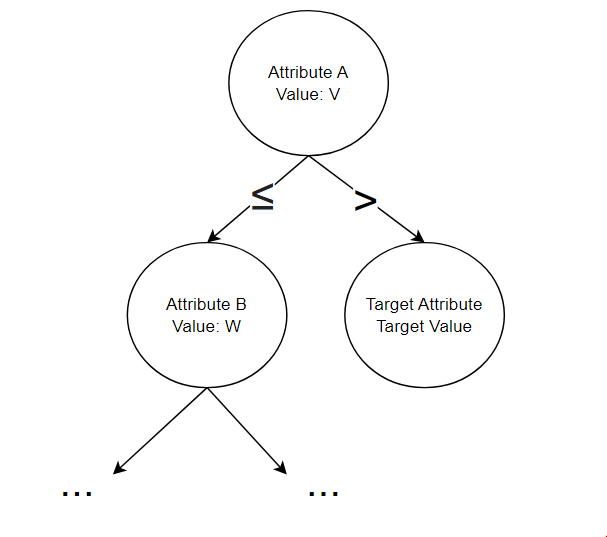
\includegraphics[scale=0.55]{images/binary-decision-tree.PNG}
    \caption{Binary decision tree created by \textit{BinaryDecisionTree} class.}
    \label{fig:binary-decision-tree}
\end{figure}

As can be seen in Figure~\ref{fig:binary-decision-tree}, leaf nodes of the tree generated by \textit{BinaryDecisionTree} have their split feature set to the target attribute of the data set, and the split feature value is the classification of the target attribute. The true and false branches are empty. As such, predictions can be made on a learned \textit{BinaryDecisionTree} for a given testing example by simply following the trees branches, checking the testing example's feature values with the split feature values at each node, until a leaf is reached where the classification for the testing example is returned.

\subsubsection{Algorithm Hyper-Parameters}
Two hyper-parameters were implemented for this Adaboost with ID3 base learner implementation. These hyper-parameters include: 1) the maximum tree depth of the learned binary decision trees, and 2) the number of weak hypotheses learned by Adaboost. 

The maximum tree depth of the learned binary decision tree is a hyper-parameter of the ID3 algorithm implementation, and it sets a limit on the maximum depth of recursion of the algorithm. This depth was monitored as a \textit{depth} parameter incremented on each recursive call. When the maximum depth was reached, the target value of majority in the current data set was returned as the leaf node. If the caller did not specify a maximum tree depth, then a tree depth of infinity was set, which essentially means the algorithm would only return a leaf node if one of its original three base cases were hit. It was experimentally determined, as can be seen in Figure~\ref{fig:depth-hyper-param}, that placing a limit on the depth of the trained binary decision tree less than the number of features in the data set actually reduces classification accuracy. For context, Figure~\ref{fig:depth-hyper-param} used a dataset with 16 features. This makes intuitive sense, as each node splits on a single feature, so there can only ever be a tree as deep as the number of features. Also, if we force a tree to terminate early, then we are forcing it to over generalize the data. Either way, this hyper-parameter remained as reducing the depth of the tree significantly improves training and classification performance. 

\begin{figure}[h]
    \centering
    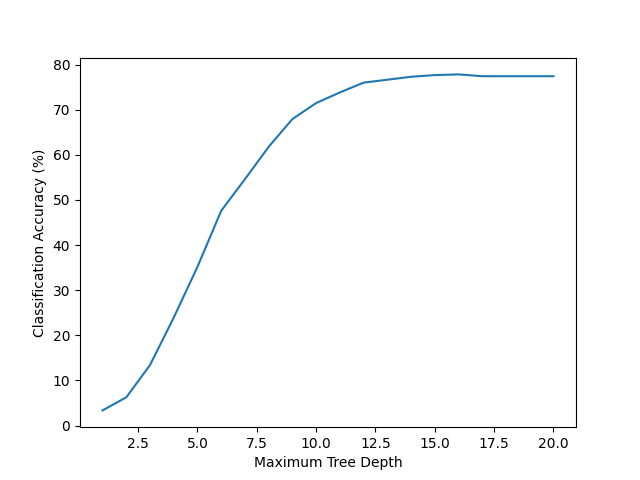
\includegraphics[scale=0.7]{images/tree-depth-plot.png}
    \caption{Accuracy of classification vs. maximum tree depth of learned binary decision tree by ID3 algorithm.}
    \label{fig:depth-hyper-param}
\end{figure}

The second hyper-parameter implemented, the number of weak hypotheses learned by the Adaboost algorithm, is a hyper-parameter of the Adaboost algorithm that controls the number of models trained by the weak base learner for a single Adaboost training session. This hyper-parameter has direct influence on the performance of the Adaboost algorithm, both from a time point-of-view and an accuracy point-of-view. The more weak hypotheses trained, the longer training will take; however, the more accurate classification can become. It was experimentally determined that 14 is the optimal number of weak hypotheses to learn as it maximizes the classification accuracy while keeping the training time as low as possible. Figure~\ref{fig:estimator-hyper-param} demonstrates how at 14 weak hypotheses, the classification accuracy of the Adaboost algorithm reaches an asymptote. Although this is only for a particular split of the dataset, it remains consistent. Figure~\ref{fig:estimator-time} shows how the time taken for training the Adaboost algorithm increases linearly with the number of weak hypotheses learned by the algorithm. As such, it is optimal to use 14 weak hypotheses to maximize classification accuracy while ensuring training time doesn't continue to increase.

\begin{figure}[h]
    \centering
    \begin{subfigure}[t]{0.48\textwidth}
        \centering
        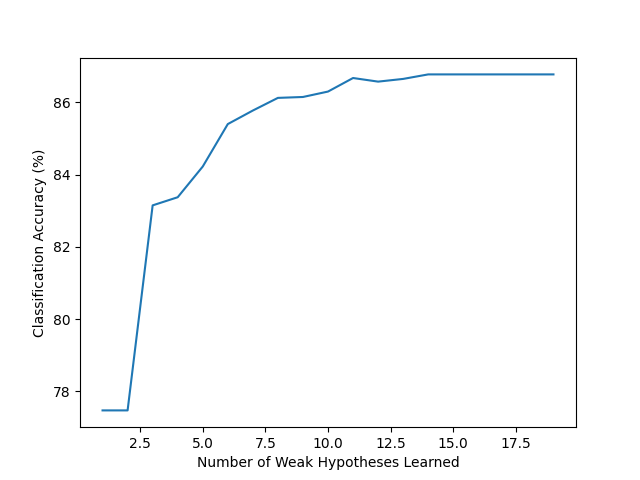
\includegraphics[width=\linewidth]{images/n-weak-hypotheses-plot.png}
        \caption{}
        \label{fig:estimator-hyper-param}
    \end{subfigure}%
    ~ 
    \begin{subfigure}[t]{0.48\textwidth}
        \centering
        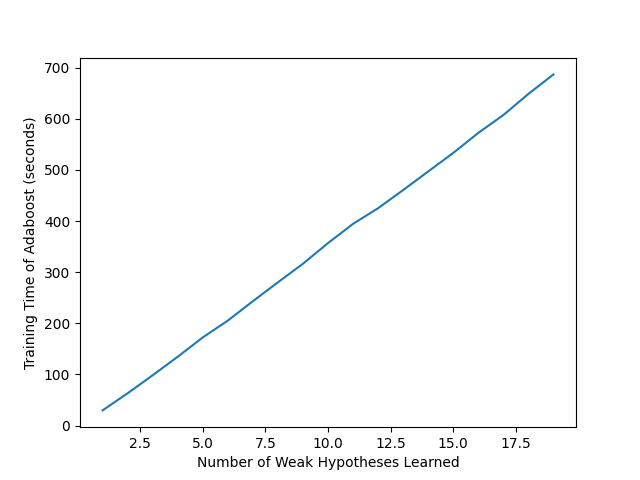
\includegraphics[width=\linewidth]{images/adaboost-training-time.png}
        \caption{}
        \label{fig:estimator-time}
    \end{subfigure}

    \caption{Performance of the number of weak hypotheses trained by Adaboost algorithm during training vs. (a) classification accuracy, and (b) time taken to train the model.}
    \label{fig:adaboost-hyper-param}
\end{figure}   

\subsection{Dataset Details}
This section will outline all details related to dataset used to train and test the Adaboost implementation. 

\subsubsection{Description of Dataset}
The dataset was taken from the UC Irvine Machine Learning Repository and has the ID 59 within this repository. The goal of the dataset is to identify each entry as a capital letter from the English alphabet based on 16 primitive numerical attributes extracted from a black-and-white image of the letter that the entry represents. The dataset contains 20 thousand entries with 17 columns for each entry, 16 columns being the previously mentioned primitive numerical attributes, and the final column being the classification of the entry, a letter in this case. These 16 primitive numerical attributes, or features in the context of machine learning, are integer values between 0 and 15 and are described as the following:
\begin{enumerate}
    \item x-box - Horizontal position of box.
    \item y-box - Vertical position of box.
    \item width - Width of box.
    \item hight - Height of box.
    \item onpix - Total number on pixels.
    \item x-bar - Mean x of on pixels in box.
    \item y-bar - Mean y of on pixels in box.
    \item x2bar - Mean x variance.
    \item y2bar - Mean y variance.
    \item xybar - Mean x y correlation.
    \item x2ybr - Mean of x * x * y.
    \item xy2br - Mean of x * y * y.
    \item x-ege - Mean edge count left to right.
    \item xegvy - Correlation of x-ege with y.
    \item y-ege - Mean edge count bottom to top.
    \item yegvx - Correlation of y-ege with x.
\end{enumerate}

The total number of classes in this dataset is 26, representing the number of capital letters in the English alphabet. The distribution of classes within the dataset is nearly uniform, as can be seen in Figure~\ref{fig:class-histogram}. As such, no re-sampling of data was needed.

\begin{figure}[h]
    \centering
    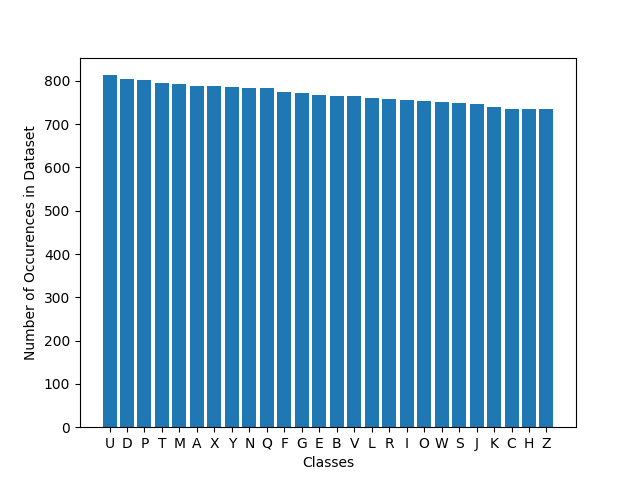
\includegraphics[scale=0.7]{images/class-distribution.png}
    \caption{Distribution of classes within the Letter Distribution dataset.}
    \label{fig:class-histogram}
\end{figure}

\subsubsection{Pre-Processing}
As previously mentioned, there are no missing values within the dataset used. As such, no pre-processing of the data to remove partial entries was required. The only pre-processing performed on the dataset was to split the data into testing and training datasets using the \textit{train\_test\_split()} function from the \textit{scikit-learn} machine learning library. A split of 80\%/20\% (16000/4000) was used for training and testing, respectively, as this was the split suggested by UC Irvine on the dataset's webpage. As such, in all results presented in the next sections, the Adaboost algorithm was trained on 16 000 randomly selected entries, and tested on the remaining 4000 entries of the dataset.

\subsection{Experimental Results}
The above discussed Adaboost algorithm with ID3 as a weak base learner implementation was tested extensively and the results of this testing can be seen in Table~\ref{tbl:adaboost-results}. As previously mentioned, these results were achieved by training the algorithm on 16 000 randomly sampled entries of the dataset, and tested on the remaining 4000 entries of the dataset. The seeds, or \textit{random\_states}, of the sampling is also reported in the table for reproducibility. The hyper-parameters were set to their previously mentioned optimal values of 16 for the maximum depth of a learned binary decision tree, and 14 for the number of weak hypotheses learned by the Adaboost algorithm.

\begin{table}[h!]
    \centering
    \begin{tabular}{||c c c c c||} 
        \hline
        Test \# & Seed & Accuracy (\%)  & Training Time (s) & Classification Time (s) \\ [0.5ex] 
        \hline\hline
        1 & 500864380 & 85.33 & 509.20 & 0.0897 \\
        \hline
        2 & 434317629 & 85.45 & 498.24 & 0.0888 \\
        \hline
        3 & 81483430 & 84.40 & 489.30 & 0.0897 \\
        \hline
        4 & 794073002 & 86.28 & 492.81 & 0.0891 \\
        \hline
        5 & 278379451 & 84.10 & 492.79 & 0.0898 \\
        \hline
        6 & 1019885152 & 84.65 & 483.37 & 0.0877 \\
        \hline
        7 & 880373647 & 85.93 & 486.33 & 0.0875 \\
        \hline
        8 & 244411609 & 85.88 & 487.19 & 0.0906 \\
        \hline
        9 & 573119018 & 83.80 & 485.92 & 0.0893 \\ 
        \hline
        10 & 496202245 & 83.03 & 487.38 & 0.0896 \\
        \hline
        11 & 136944384 & 84.18 & 500.03 & 0.0905 \\
        \hline
        12 & 131276866 & 85.80 & 486.27 & 0.0868 \\
        \hline
        13 & 276617434 & 86.70 & 482.18 & 0.0886 \\
        \hline
        14 & 817708150 & 86.60 & 478.75 & 0.0892 \\
        \hline
        15 & 44078284 & 86.68 & 505.69 & 0.0908 \\ [1ex]
        \hline
    \end{tabular}
    \caption{Results of training Adaboost implementation on 16 000 randomly sampled examples and classifying the remaining 4000 examples with maximum tree depth of 16 and 14 weak base hypotheses learned.}
    \label{tbl:adaboost-results}
\end{table}

The mean classification accuracy of the results presented in Table~\ref{tbl:adaboost-results} is 85.254\%, with the mean training and classification times being 491.03 seconds and 0.08918 seconds, respectively. Despite not achieving 100\% accuracy, the Adaboost implementation is still a success in our opinion as it is a completely from scratch implementation. The lack of accuracy in classification may come from the weighted feature info gain calculation being employed, referenced in Equation~\ref{eq:weighted-info-gain}, to place more emphasis on previously incorrectly classified examples. As for the training time, ID3 is a greedy algorithm, as such it is expected to have a longer execution time. Much work was done in the ID3 implementation to ensure all math operations were vectorized within the Python programming language to minimize the amount of looping and memory copies required. No parallelization was employed as to not over complicate the implementation, yet the routine for determining the split feature can easily be parallelized as determining the split feature based on weighted info gain can be done independently of other features.

The confusion matrix of the test with the highest accuracy, test 13 with seed 276617434, can be seen in Figure~\ref{fig:confusion-matrix}. The confusion matrix helps highlight the number of examples that were incorrectly classified, and what those incorrect classifications were compared to the correct classifications. As such, a strong diagonal of the matrix indicates high classification accuracy, as can be seen in Figure~\ref{fig:confusion-matrix}.

\begin{figure}[h!]
    \centering
    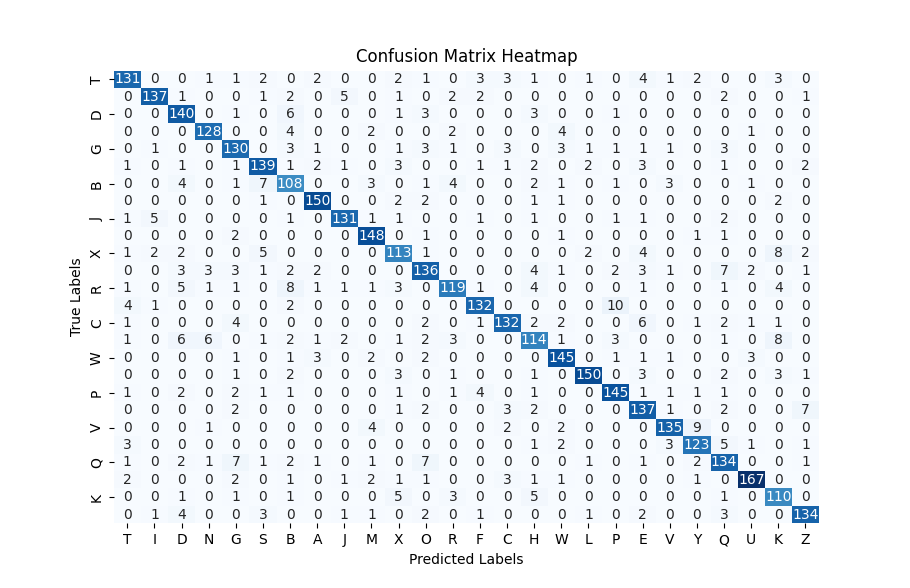
\includegraphics[scale=0.65]{images/confusion-matrix.png}
    \caption{Confusion matrix of training/classification results with seed 276617434.}
    \label{fig:confusion-matrix}
\end{figure}


\newpage

\section{ANN with Backpropagation}

An Artificial Neural Network with backpropagation was successfully implemented using the Python 3 programming language. The artificial neural network that was created featured a simplistic design, utilizing only one hidden layer while simultaneously yielding great results. This algorithm was trained on a dataset that consisted of features computed from digitized images of fine needle aspirate of breast mass, describing charactersitics of the cell nuclei present in the image. The objective was classification of cell mass as either benign or malignant.

\subsection{Artificial Neural Networks}
\label{ANNTheory}

As mentioned, this section of the programming project saw the implementation of an artificial neural network from scratch. Artificial neural networks, or neural networks, are a machine learning technique that seek to mimic the biological neural networks found within human brains. A neural network consists of connected ``units", or nodes, that are called neurons. These neurons are designed such that they mimic the neurons found within a human brain, in the sense that they will not ``fire'', so to speak, if the input signal is not larger than a certain threshold. This thresholding is achieved through the use of an activation function, which ensures that important features that are interesting enough to be learned are actually learned by the network as they exceed the threshold. The output of a given neuron is therefore calculated by applying the activation function to the weighted sum of the inputs to that neuron. Neural networks are composed of three distinct layers, those being the input layer, the hidden layer, and the output layer. The input signal is first sent through the input layer, which takes in the data and sends it to the subsequent layers, known as the hidden layers. The hidden layers serve as an intermediary layer between the first layer and the last layer, the output layer. It is within these hidden layers that the input becomes further and further abstracted, and a new representation is learned that extracts the hidden relationship between the input features. 


For this assignment, as mentioned, a neural network was created with three layers: one input, one hidden, and one output. Justification for the choice of this structure can be found within Section \ref{ANNhyperparameterselection}. As such, the general structure of the neural network implemented is given by Figure \ref{fig:annstructure}:

\begin{figure}[h]
    \centering
    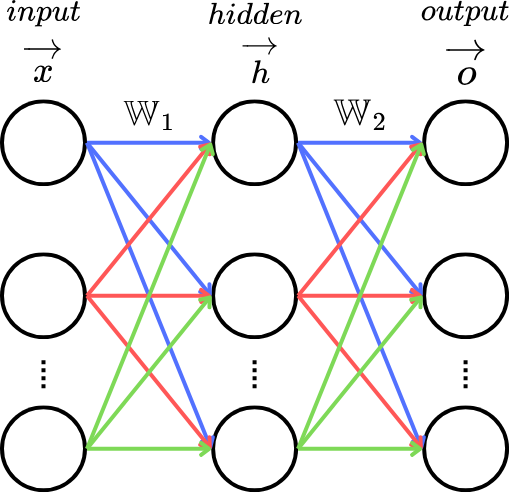
\includegraphics[scale = 0.5]{images/annstructure.png}
    \caption{Structure of the ANN that was developed.}
    \label{fig:annstructure}
\end{figure}

Where a vector of inputs $\overrightarrow{x}$ is fed into the first layer of the network, and this vector is then multiplied by the matrix of weights for the connections between the input layer and the hidden layer, $\mathbb W_1$. There is also a bias that gets added to this weighted summation, denoted by $\overrightarrow{b_1}$. This process results in what is known as the net, which is the weighted summation that is fed into the activation function of the first hidden layer. This is given by Equation \ref{eq:net1} below:

\begin{equation}
    \label{eq:net1}
    \overrightarrow{net_{1}} = \mathbb W_{1} \times \overrightarrow{x} + \overrightarrow{b_1}
\end{equation}

Following the determination of $\overrightarrow{net_{1}}$, this value is then fed into the hidden layer and the activation function is applied, which is given below by Equation \ref{eq:h1}:

\begin{equation}
    \label{eq:h1}
    \overrightarrow{h} = \sigma(\overrightarrow{net_{1}})
\end{equation}

Equation \ref{eq:h1} yields the output from the hidden layer, which is then multiplied by the weights between the hidden and output layer and added to another bias vector to get another net, shown below as:

\begin{equation}
    \label{eq:net2}
    \overrightarrow{net_{2}} = \mathbb W_{2} \times \overrightarrow{h} + \overrightarrow{b_2}
\end{equation}

Finally, the output of the network is computed by applying the activation function to $\overrightarrow{net_{2}}$, as given by:

\begin{equation}
    \label{eq:o1}
    \overrightarrow{o} = \sigma(\overrightarrow{net_{2}}) 
\end{equation}

Neural networks learn by continually updating their weights through a process known as backpropagation, which involves taking the gradient of the difference between your target value and output value, with respect to each individual weight matrix $\mathbb W_{i}$. To update the weights, we want to learn $\mathbb W$'s that minimize the square error function, given by:

\begin{equation}
    \label{eq:squarederrorfunction}
    E[\mathbb W] = \frac{1}{2} \sum_{d \in D}(t_d - o_d)^2
\end{equation}

Where $d$ represents an example from the dataset $D$, $t_d$ is the target label for that example, and $o_d$ is the output of the network. By calculating the gradient of this error function, we get:

\begin{equation}
    \label{eq:sqegradient}
    \nabla{E[\mathbb W]} = \left[ \frac{\partial{E}}{\partial{\mathbb W_o}}, \frac{\partial{E}}{\partial{\mathbb W_1}}, \ldots, \frac{\partial{E}}{\partial{\mathbb W_n}} \right]
\end{equation}

To train the network, we must update the weights according to the following equation:

\begin{equation}
    \label{eq:trainW}
    \mathbb W_i = \mathbb W_i + \Delta{\mathbb W_i}
\end{equation}

Where the incremental change in weight, $\Delta{\mathbb W_i}$, is given by the following equation:

\begin{equation}
    \label{eq:deltaW}
    \Delta{\mathbb W_i} = -\eta \frac{\partial{E}}{\partial{\mathbb W_i}}
\end{equation}

Where $\eta$ is the \textit{learning rate}, which determines the size of the step to be taken during the gradient descent algorithm. The value of $\frac{\partial{E}}{\partial{\mathbb W_i}}$ is given by the following derivation:

\begin{gather}
    \begin{aligned}
        \frac{\partial{E}}{\partial{\mathbb W_i}} &= \frac{\partial}{\partial{\mathbb W_i}} \frac{1}{2} \sum_{d \in D}(t_d - o_d)^2 \\
        &= \frac{1}{2}\sum_{d \in D}\frac{\partial}{\partial{\mathbb W_i}}(t_d - o_d)^2 \\
        &= \sum_{d \in D}(t_d - o_d)\frac{\partial}{\partial{\mathbb W_i}}(t_d - o_d) \\
        &= \sum_{d \in D}(t_d - o_d)\left[-\frac{\partial{o_d}}{\partial{\mathbb W_i}}\right] \\
        &= -\sum_{d \in D}(t_d - o_d)\left[\frac{\partial{o_d}}{\partial{\mathbb W_i}}\right] \\
        \therefore \frac{\partial{E}}{\partial{\mathbb W_i}} &= \sum_{d \in D}(o_d - t_d)\left[\frac{\partial{o_d}}{\partial{\mathbb W_i}}\right]
    \end{aligned}
\end{gather}

Where the value of $\sum_{d \in D}(o_d - t_d)$ is equal to the gradient of the error with respect to the output value $o_d$, as evidenced by Equation \ref{eq:delEdelod}:

\begin{gather}
    \begin{aligned}
        \label{eq:delEdelod}
        \frac{\partial{E}}{\partial{o_d}} &= \sum_{d \in D}(o_d - t_d) \\
        \frac{\partial}{\partial{o_d}}\frac{1}{2}\sum_{d \in D}(t_d - o_d)^2 &= \sum_{d \in D}(o_d - t_d) \\
        \sum_{d \in D}(t_d - o_d)(-1) &= \sum_{d \in D}(o_d - t_d)\\
        \therefore \sum_{d \in D}(o_d - t_d) &= \sum_{d \in D}(o_d - t_d)
    \end{aligned}
\end{gather}

From this, it can be gathered that to update any $\mathbb W_i$, we can use the following equation:

\begin{equation}
    \label{eq:keyweightupdating}
    \mathbb W_i = \mathbb W_i - \eta \left[ \frac{\partial{E}}{\partial{o_d}}\times\frac{\partial{o_d}}{\partial{\mathbb W_i}} \right]
\end{equation}

Meaning that for each layer, the value of $\frac{\partial{o_d}}{\partial{\mathbb W_i}}$ needs to be determined such that each weight matrix can be updated. For the second weight matrix, this derivation is given by Equation \ref{eq:w2update}. The $d$ subscript is dropped as it was assumed that stochastic gradient descent would be employed, which obviously is performed on each training example $d \in D$.

\begin{gather}
    \begin{aligned}
        \label{eq:w2update}
        \frac{\partial{o}}{\partial{\mathbb W_2}} &= \frac{\partial}{\partial{\mathbb W_2}}\sigma(\overrightarrow{net_2}) \\
        &= \frac{\partial}{\partial{\mathbb W_2}}\sigma(\mathbb W_2 \sigma(\mathbb W_1 \overrightarrow{x})) \\
        \therefore \frac{\partial{o}}{\partial{\mathbb W_2}} &= \sigma'(\overrightarrow{net_2})h
    \end{aligned}
\end{gather}

Similarly, this process was repeated for $\mathbb W_1$:

\begin{gather}
    \begin{aligned}
        \label{eq:w1update}
        \frac{\partial{o}}{\partial{\mathbb W_1}} &= \frac{\partial}{\partial{\mathbb W_1}}\sigma(\overrightarrow{net_2}) \\
        &= \frac{\partial}{\partial{\mathbb W_1}}\sigma(\mathbb W_2 \sigma(\mathbb W_1 \overrightarrow{x})) \\
        &= \sigma'(\overrightarrow{net_2})\frac{d}{d{\mathbb W_1}}\left[ \mathbb W_2 \sigma(\mathbb W_1 \overrightarrow{x}) \right]\\
        \therefore \frac{\partial{o}}{\partial{\mathbb W_1}} &= \sigma'(\overrightarrow{net_2})\mathbb W_2 \sigma'(\overrightarrow{net_1})\overrightarrow{x}
    \end{aligned}
\end{gather}

The question therefore arose, how will the bias be updated? It was determined that the bias would be updating using a similar approach to Equation \ref{eq:trainW}, where the bias updating equation is given below as:

\begin{equation}
    \label{eq:trainBias}
    b_i = b_i - \eta \frac{\partial{E}}{\partial{b_i}}
\end{equation}

Where the partial derivative of error with respect to the bias value $b_i$ is given by:

\begin{gather}
    \begin{aligned}
        \label{eq:biasderivation}
        \frac{\partial{E}}{\partial{b_i}} &= \frac{\partial}{\partial{b_i}}\left[ \frac{1}{2} \sum_{d \in D}(t_d - o_d)^2 \right] \\
        &= \frac{1}{2}\sum_{d \in D} \frac{\partial}{\partial{b_i}}(t_d - o_d)^2 \\
        &= \sum_{d \in D}\frac{\partial}{\partial{b_i}}(t_d - o_d) \\
        &= \sum_{d \in D}(t_d - o_d)\frac{\partial}{\partial{b_i}}(-o_d) \\
        \therefore \frac{\partial{E}}{\partial{b_i}} &= \sum_{d \in D}(o_d - t_d)\frac{\partial{o_d}}{\partial{b_i}}
    \end{aligned}
\end{gather}

Where the value of $\sum_{d \in D}$ is known by Equation \ref{eq:delEdelod}, which implies that the partial derivative of error with respect to bias is equal to:

\begin{equation}
    \label{eq:delEdelbias}
    \frac{\partial{E}}{\partial{b_i}} = \frac{\partial{E}}{\partial{o_d}} \times \frac{\partial{o_d}}{\partial{b_i}}
\end{equation}

The expanded equation of the output from our network, with biases included, is given below within Equation \ref{eq:outputwithbias}. The biases were initially neglected when determining the weight matrices as they are not functions of the weight, and therefore were dropped when the partial derivative of error with respect to the weight matrices was performed. 

\begin{equation}
    \label{eq:outputwithbias}
    \overrightarrow{o} = \sigma(\mathbb W_2 \sigma(\mathbb W_1 \overrightarrow{x} + \overrightarrow{b_1}) + \overrightarrow{b_2})
\end{equation}

Therefore, we just need to determine the value of $\frac{\partial{o_d}}{\partial{b_i}}$ for each layer. For $b_2$, this is done as follows:

\begin{gather}
    \begin{aligned}
        \frac{\partial{o_d}}{\partial{b_2}} &= \frac{\partial}{\partial{b_2}}\sigma(\overrightarrow{net_2} + \overrightarrow{b_2}) \\
        \frac{\partial{o_d}}{\partial{b_2}} &=\sigma'(\overrightarrow{net_2})
    \end{aligned}
\end{gather}

For $b_1$, this is done as follows:

\begin{gather}
    \begin{aligned}
        \frac{\partial{o_d}}{\partial{b_1}} &= \frac{\partial}{\partial{b_1}} \sigma(\mathbb W_2 \sigma(\mathbb W_1 \overrightarrow{x} + \overrightarrow{b_1}) + \overrightarrow{b_2})\\
        \frac{\partial{o_d}}{\partial{b_1}} &= \sigma'(\overrightarrow{net_2})\mathbb W_2 \sigma'(\overrightarrow{net_1})
    \end{aligned}
\end{gather}

The general workflow for utilizing the neural network is as follows:

\begin{enumerate}
    \item A neural network object is instantiated from a class, specifying the input size, the hidden layer size, and output size.
    \item This network is then trained, using a training function that is contained within the object. This training procedure calculates a forward pass first by passing the input vector through the network, which yields an output. This output, as well as the target values from the input vector and a learning rate are passed through a backward pass, which updates the weights using the backpropagation equations determined above.
    \item Once the network has been trained, it can be tested by passing it features and labels, where it calculates the accuracy of the model based on how many it correctly classifies.
\end{enumerate}

With all of the pertinent equations for the backpropagation algorithm determined, as well as the workflow, the focus then turned towards the actual implementation of the neural network through code for performing classification on the given dataset.

\subsection{Implementation Details}

This section outlines all details related to the implementation of the neural network, including the development platform and libraries used, the programmatic structure, the data structures used, and the choice of hyperparameters.

\subsubsection{Development Platform \& Libraries Used}

As was previously mentioned, all code written to implement the neural network with backpropagation was written in Python 3. The code was written on a Windows operating system, and was not tested on other operating systems, but it is assumed that it will run on any system that can run the Python programming language. The development of this algorithm was done using Microsoft's Visual Studio Code. The environment was configured to run Jupyter Notebook .ipynb files, which due to their ability to run code one cell at a time, are favoured for machine learning development. The Python 3 kernel that was utilized within this .ipynb environment was Python 3.12.5. Code versioning was controlled through Git utilizing a remote repository hosted on GitHub. The neural network itself, as well as the backpropagation algorithm, were written completely from scratch using Python's built-in functionalities as well as the \textit{Numpy} Python library for mathematical operations. The \textit{Pandas} Python library was utilized for data manipulation and exploratory analysis, and the \textit{scikit-learn} machine learning Python library was used to apply pre-processing to the data, as well as performing the train/test split. It must be noted that this machine learning library was not used for anything other than splitting data and applying standardization. It was not incorporated within the actual neural network class, and did not contribute to the development of the neural network other than being a tool for data separation and scaling. The \textit{matplotlib} and \textit{seaborn} Python libraries were utilized for visualization of both training and testing results, and the \textit{csv} python package was used to save initial weights when a good run occurred and load them to initialize the network. Finally the UC Irvine Machine Learning Python package \textit{ucimlrepo} was used to fetch the dataset, which was hosted on their website. 

\subsubsection{Program Structure}

The neural network code was implemented using a .ipynb file within VS Code, as mentioned previously. This meant that the code could be partitioned into sections, and each section must be run sequentially for the code to function. The sections are as follows:

\begin{enumerate}
    \item Importing Packages
    \item Loading the Dataset
    \item Examining the Dataset Properties
    \item Dataset Pre-Processing
    \item Function Definition
    \item Training \& Testing the Model
\end{enumerate}

The general workflow of the program is as follows. Firstly, the relevant packages necessary to utilize the code are imported. Following this, the dataset is fetched from the UC Irvine Machine Learning repository. An exploratory analysis is performed on the data, which gets the total number of instances, the number of features, the number of unique target variables, and the names of each feature. Following this, the dataset is pre-processed, where it is examined for null values and standardized, and the labels are binary encoded from categorical values. Several functions are defined, as well as the main neural network class. A sigmoid function and its derivative were defined, as well as a ReLu function and its derivative. A binary cross entropy loss function was defined since the classification task is binary in nature. Following this, the neural network class was defined.

As previously mentioned, an object-oriented approach was implemented for the neural network architecture. This allowed training, testing, and instantiating the network to be done utilizing functions inherent to the class. The class contains a constructor that takes the number of input neurons, the number of hidden neurons, and the expected output size. Within this constructor, weights are randomly initialized from a normal distribution. A feedforward function was defined that takes in the vector of inputs, and ensures that this vector is a column vector. Following this, the net and activated net are calculated for each layer, and the output is returned. A backpropagation function was defined that performs the backpropagation procedure for every weight and bias value, in accordance with the equations derived in Section~\ref{ANNTheory}.

The neural network class also contains training and testing functions. The training function takes in the training x and y values, as well as the validation x and y values, a number of epochs, and a learning rate. This training function utilizes every feature and computes the forward pass and back propagates for every example, for every epoch. In this regard, the training process utilizes stochastic gradient descent. The average binary cross entropy across all training examples per epoch is calculated as a loss metric, and a similar process occurs for validation data. This function returns the training loss history and the validation loss history. 

The testing function effectively computes the forward pass, and extracts a class value from the sigmoid layer result, and if this predicted value is the same as the target, it increments the number of correct predictions. Accuracy is calculated as the number of correct predictions divided by the number of testing values examined. With the pertinent functions defined, a network is instantiated from the class, and it is trained using the training and validation data. Following this, the training and validation loss is plotted with respect to epochs, and the network is tested. A confusion matrix is generated to visualize the efficacy of the model. This entire process can be run by selecting ``run all" within the .ipynb file.


\subsubsection{Data Structures Used}

When the data is initially fetched from the remote repo, it is imported as a special data structure called \textit{ucimlrepo.dotdict.dotdict}. This data type seems to be a dictionary of Pandas data frames because the feature and target values are stored within Pandas data frames. As mentioned previously, Pandas data frames were used extensively throughout this project due to their ease of manipulation and representation. This data frame structure allowed for exploratory analysis to be performed on the feature data, and the dataset could be examined in terms of how many instances there were, the number of features, the number of unique target variables, and the name of the features. A Pandas data frame also allows for using the \textit{.head()} handle to examine the first five rows of data, which allowed for quick visualization as the data was manipulated.

Numpy arrays were utilized within the forward and backward pass operations due to their ease of mathematical computation and speed of computation compared to Pandas data frames. These arrays were also utilized to store the weights, biases, and activated nets of the network due to the mathematical operations to be performed using them. Data was fed into the network by extracting each row of the data frame and converting it to a Numpy column vector. Finally, lists were utilized to store the training and validation loss history, as well as the correct predictions and target values used in formulating the confusion matrix.

\subsubsection{Hyperparameter Selection}\label{ANNhyperparameterselection}

As was mentioned, the network designed had three layers: an input layer, a singular hidden layer, and an output layer. It was decided that the network would have one hidden layer for ease of formulation, and because of the simplicity of the binary classification task to be performed. Having one hidden layer made deriving the backpropagation equations simpler, as only four equations had to be determined: two for weights and two for biases. The network was able to extract the required relationships for correctly classifying a cell mass as benign of malignant at just one layer. As such, it was deemed that a single hidden layer was enough. It was decided that the activation function to be used within the hidden layer was to be a ReLu function, and the activation function to be used at the output was a sigmoid. The ReLu function was chosen to potentially combat any problems related to updating the weights, and the probabilistic sigmoid function was chosen because the classification task to be performed was binary, and the sigmoid function is capable of outputting within a range between 0 and 1. 

Therefore, the hyperparameters explored were the number of epochs, the learning rate, and the number of neurons within the hidden layer. 10 hyperparameter combinations were explored, and the average accuracy after 5 runs was recorded for each combination. This process was done to determine which hyperparameter combination had a higher accuracy on average, as that would lead to the best model performance. All of these tests were performed by randomly sampling the weights from a normal distribution, which had the downside of a fluctuating accuracy that could perform very poorly if the initial weights used for gradient descent were poor. This process then allowed for determining a good set of initial weights and biases, which were then flattened and stored into a CSV that is now loaded every time the model is ran. This hyperparameter analysis was therefore utilized to determine the best combination of hyperparameters and the best initial weights to be used. Weights and biases are not hyperparameters, but the combination of hyperparameters that produced the best accuracy was then examined further to determine the best initial weights. The results of this hyperparameter analysis are shown below within Table \ref{tbl:hyperparametertesting}.
\newpage

\begin{table}[h!]
    \centering
    \begin{tabular}{||c c c c c||} 
        \hline
        Test \# & Epochs & $\eta$ & \# Hidden Neurons & Average Accuracy (\%) \\ [0.5ex] 
        \hline\hline
        1 & 1000 & 0.0001 & 30 & 91.99 \\
        \hline
        2 & 1000 & 0.00025 & 30 & 94.65 \\
        \hline
        3 & 1000 & 0.0005 & 30 & 93.72 \\
        \hline
        4 & 1000 & 0.001 & 30 & 96.28 \\
        \hline
        5 & 1500 & 0.0001 & 30 & 93.67 \\
        \hline
        6 & 1500 & 0.00025 & 30 & 96.05 \\
        \hline
        7 & 1500 & 0.0005 & 30 & 95.81 \\
        \hline
        8 & 1500 & 0.001 & 30 & 95.35 \\
        \hline
        9 & 1000 & 0.001 & 15 & 96.28 \\ 
        \hline
        10 & 1000 & 0.001 & 45 & 94.88 \\
        \hline
    \end{tabular}
    \caption{Average accuracy after 5 trials for each hyperparameter combination explored.}
    \label{tbl:hyperparametertesting}
\end{table}

The highest average accuracy after 5 runs was exhibited by Test 4, which was trained at 1000 epochs, a learning rate of 0.001, and had 30 hidden nodes. It was generally observed that as the number of hidden nodes increased, the accuracy fell. Lower numbers of hidden nodes had sporadic accuracy that varied greatly, with outliers that were omitted from the average accuracy calculation. This combination of hyperparameters was capable of producing an accuracy that was as high as 98.837\%, the highest accuracy that was exhibited. The initial weights and biases from this 98.837\% test run were saved as a CSV, and the neural network class was updated to include an option to utilize the saved weights. If the user does not want to load the weights, the weights and biases are randomly sampled.

\subsection{Dataset Details}

The dataset used was from the UC-Irvine Machine Learning Repository and was donated by the University of Wisconsin-Madison in 1995. It is considered a multivariate dataset, consisting of several breast mass features that were computed from digitized images of fine needle aspirate. These features describe the characteristics of the cell nuclei present within a given image. 10 real-valued features are of importance for this dataset, those being:

\begin{enumerate}
    \item radius (mean distances from the center to points on the perimeter)
    \item texture (standard deviation of gray-scale values)
    \item perimeter of the cell mass
    \item area of the cell mass
    \item smoothness (local variation in radius lengths)
    \item compactness (measured by dividing the squared perimeter by the area, and subtracting 1)
    \item concavity (severity of concave portions of the contour)
    \item concave points (number of concave portions of the contour)
    \item symmetry of the cell mass
    \item fractal dimension (statistical metric for complexity, measured using the ``coastline approximation" - 1)
\end{enumerate}

For each of these real-valued features, there are 3 versions. These versions represent the mean, standard deviation, and worst-case value of each feature. In total, there are 30 features in this dataset. The target variable within this dataset is a diagnosis, either benign or malignant, which are represented categorically as either a B or an M, respectively. There were 569 examples within this dataset. The dataset was loaded using the UCI-ML \textit{fetchrepo} command and was subsequently ready for processing. 

\subsection{Data Pre-processing}

As mentioned, the dataset was loaded using the \textit{fetch\_ucirepo} command from the UCI-ML Python package. This command fetched the dataset from the UCI website, utilizing its intrinsic dataset ID, which was 17. This data was saved into a variable called \textit{breast}, as a unique class from the UCI-ML package, called \textit{ucimlrepo.dotdict.dotdict}, which is seemingly a dictionary-based class. This data was then split into features and target labels, by calling either \textit{.data.features} or \textit{.data.targets}, respectively. The feature values were saved into a Pandas data frame called \textit{breast\_x}, whereas the target values were saved into a Pandas data frame called \textit{breast\_y}. Following the importing and analysis of the Wisconsin Breast Cancer dataset, there arose a need to pre-process the data, as is the case with most machine learning applications. The pre-processing that was performed was an inquiry into the existence of null values, standardization of the values such that their values fell within a common range, and the categorical labels were encoded into binary 0 or 1, where 0 represents benign, and 1 represents malignant. 

Null values were examined using the \textit{.isnull()} handle for Pandas data frames, combined with the \textit{.values.any()} handle from Python. This returned either True for null values, or False if no null values existed. If any null values were found within the dataset, the \textit{.dropna()} handle for Pandas data frames was used to remove all null values. This process was repeated for both the features and target values. Following this, the feature value was standardized. This was performed as the features of the input dataset had vast differences between their ranges, since different units were used for different features, as some measurements pertained to distances whereas some measurements pertained to areas or dimensionless concepts such as texture. The \textit{StandardScaler()} function from \textit{sklearn} was utilized to standardize the feature data. Finally, the categorical variables were encoded by indexing the ``Diagnosis" column of the target data frame, and mapping the value to 1 if the row value was ``M", and 0 if else. This effectively encoded the categorical data into a binary encoding suitable for use in a neural network. Following this, the dataset was split into 70\% training and 30\% testing/validation, which was then split using a 50-50 split. The entirety of this process can be seen within Appendix \hl{INSERT APPENDIX REF}.

\subsection{Experimental Results}

After detailing the theoretical background for the ANN structure, the libraries, platform, and data structures used, as well as the process of determining hyperparameters and analyzing the data set, it was thus time to test the dataset. Utilizing the hyperparameters and initialized weights determined in Section \ref{ANNhyperparameterselection}, the model was trained on the training data and the loss for both training and validation was visualized. Following this, the model was tested against the test dataset and a confusion matrix was generated to visualize its efficacy. To evaluate the model, the code was ran 10 times and the average accuracy was calculated. This meant that 10 models were generated with initialized weights, utilizing the same hyperparameters, and tested against a test set that was unique to that run. The average accuracy of the model after experimental evaluation was 95.56\%, with the highest measured accuracy being 98.837\%, and the lowest accuracy being 91.86\%. The training results and testing confusion matrix of the highest run are shown within Figures \ref{fig:anntrain} and \ref{fig:anncm}, respectively. 

\begin{figure}[h]
    \centering
    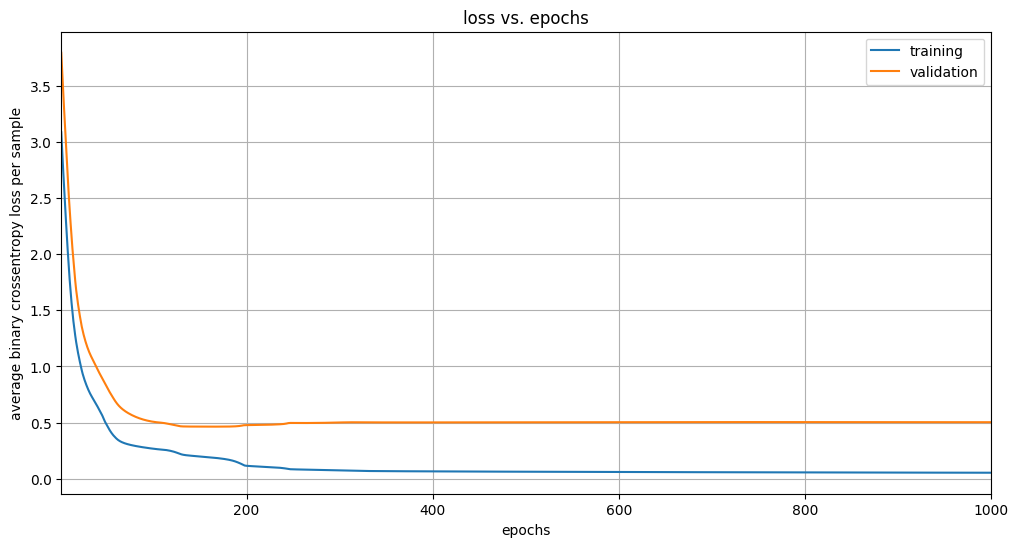
\includegraphics[width=0.9\linewidth]{images/ANNtrain.png}
    \caption{Training results of the best run for testing the ANN.}
    \label{fig:anntrain}
\end{figure}

\begin{figure}[h]
    \centering
    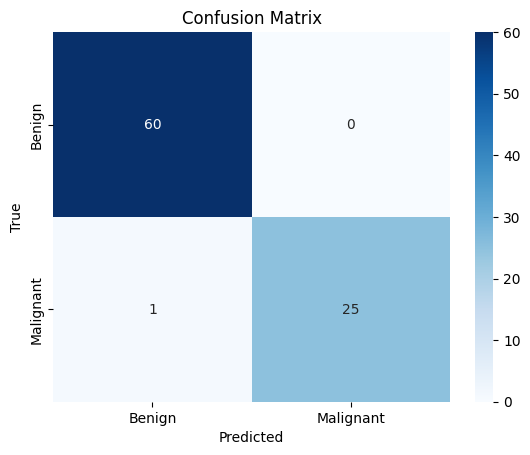
\includegraphics[width=0.8\linewidth]{images/ANNcm.png}
    \caption{Confusion matrix results of the best run for testing the ANN.}
    \label{fig:anncm}
\end{figure}
\newpage

Overall, we are satisfied with the performance of the neural network. The developers of the dataset report an average accuracy of 92.308\% utilizing a neural network for classification, and for this neural network implementation developed from scratch, we are more than happy to find that we have exceeded this value. Loading the initialized weights and biases helped tremendously in the accuracy of the model by removing the possibility of severely low weights. Before initializing the weights from a set of pre-determined weights, there were instances where the test accuracy would be exceedingly low, as low as 65\% due to poor random sampling of initial weights. This would cause the training loss to never come down and approach a value close to zero, and as such the model performed quite poorly. By initializing the weights to a good initial guess, even when the model performed poorly it only reached a low accuracy of 91.86\%, far better than 65\%. The accuracy fluctuates around $\sim$ 95\% currently, and the performance varies due to the random nature of training using backpropagation and stochastic gradient descent. Because the training data is also randomized when it is split, some training runs might see examples with easy-to-extract relationships initially, whereas others might have closely related values that are not easy to determine.

This model also has its performance capped due to only having 1 hidden layer, and might even realize higher levels of accuracy with a deeper network, but the average accuracy for this model was deemed to be sufficient for this application. As seen within Figure \ref{fig:anntrain} the model does not seem to be overfitting, as evidenced by the validation loss that steadily plateaus instead of increasing. The confusion matrix for the best test, as shown in Figure \ref{fig:anncm}, showcases that even for a partially imbalanced test set, the model is still able to realize high performances. Future work for this model could entail utilizing a deeper network, or processes such as dropout, regularization, or the use of batches.

\section{Naive Bayes for Car Evaluation}
In this section of the report, the team implemented a Naive Bayes (NB) classifier from scratch and investigated the performance of the algorithm. In essence, NB classifiers are a machine learning model that learns the probability distribution in the training data under the naive assumption that the data features are conditionally independent. Therefore, the algorithm is a simple implementation of Bayesian networks. This section starts with a review of the theory and mechanism of NB classifiers, followed by a description of the car evaluation dataset, NB classifier implementation, finally the results and discussion of results.

\subsection{Naive Bayes Classifier Theory}

To assist in the formulation of an NB classifier, assume a dataset that contains training instances, each defined by a feature vector of \textit{n} features $\vec{x}=(x_1, x_2, \cdots x_n)$ and a class value, $C$. NB classifiers are ideal when working with categorical features. The NB classifier is trained to classify a test example based on its feature values and the probability distribution provided in the training set. NB classifier operates based on Bayes theorem, formulated as:

\begin{equation} \label{eq:Bayes_theorem}
    p(C_k|\vec{x}) = \frac{p(C_k)p(\vec{x}|C_k)}{p(\vec{x})}
\end{equation}

where $p(C_k|\vec x)$ represents the probability of a class, $C_k$, given the input features, $p(C_k)$ is the prior probability of the class from the data set, $p(\vec x|C_k)$ is the likelihood of the feature vector given the class, and $p(\vec x)$ is the evidence probability. Bayes Theorem plays an important role in Bayes classifiers since it allows for the classification of new data samples by leveraging the known distribution from the dataset. The left expression in \cref{eq:Bayes_theorem} is the quantity of interest since one can determine the probability of each class given the feature vector $\vec {x}$ and classify the instance as the class with the highest probability. The probability of each class given a data sample has the same denominator, $p(\vec x)$, as a normalizing factor. This can be simplified when considering the relative probabilities among classes.

\begin{equation} \label{eq:Bayes_theorem_simplified}
    p(C_k|\vec{x}) \propto p(C_k)p(\vec{x}|C_k)
\end{equation}

However, the left expression is challenging to obtain compared to the probabilities in the right expression. The prior probability $p(C_k)$ is the proportion of training samples with the class $C_k$ in the dataset. The likelihood $p(\vec x|C_k)$ is the number of samples of class $C_k$ with the features of $\vec x$. However, the curse of dimensionality presents the biggest drawback of this method. Computation time increases exponentially with the number of features. This quantity is further simplified in Naive Bayes with the assumption of conditional probability. Under this assumption, the features are independent when given the class label. Mathematically, this assumption simplifies the joint probability of the likelihood, $p(\vec x|C_k)$, to the product of individual conditional probabilities as:

\begin{equation}
\begin{aligned}
    p(\vec x|C_k) &= p(x_1, x_2 , ... , x_n|C_k) = p(x_1|C_k)\times p(x_2|C_k) \times ... p(x_n|C_k) \\
    p(\vec x|C_k) &= \prod_{i=1}^n p(x_i|C_k)
\end{aligned}
\end{equation}

With this simplifying assumption, computation time only increases linearly with the number of features compared to the joint probability calculation. The expression in \cref{eq:Bayes_theorem_simplified} is then further simplified as:

\begin{equation}
     p(C_k|\vec{x}) \, \propto \, p(C_k) \prod_{i=1}^n p(x_i|C_k)
\end{equation}

\subsection{Implementation of Naive Bayes Classifier}

\subsubsection{Platform} \label{subsubsec:platform}

A Naive Bayes Classifier algorithm was developed using Python in the Visual Studio Code development environment. The code was implemented in the form of code blocks in a Jypyter notebook and versioning was handled using Git to the main project repository. The Naive Bayes classifier and the helper functions were developed from scratch and employed Python built-in libraries for efficient numerical handling. More specifically

\begin{itemize}
    \item \lstinline{ucimlrepo} - for importing the car dataset
    \item \lstinline{pandas} - for working with data frames and related tasks, such as statistics, sample counting, ...
    \item \lstinline{sklearn} - for splitting the dataset into train and test set and evaluation scoring metrics 
    \item \lstinline{matplotlib} - for visualizing for 
    \item \lstinline{collection} - to import the \lstinline{defaultdict} construct to define empty nested dictionary for the individual conditional probabilities
\end{itemize}

\subsubsection{Dataset Description}
From the data discovery steps, the original dataset contains 1727 instances. Each instance has six categorical features - buying price, maintenance cost, number of doors, passenger capacity, size of the lug boot, and safety - encoded as 

\begin{itemize}
    \item buying: The buying price has 4 categories - low, med, high, and high
    \item  maint: The maintenance price has the similar 4 categories
    \item doors: The number of doors has 4 categories - 2, 3, 4, and 5more
    \item person: The number of passenger capacity has 3 categories - 2, 4, and more
    \item lug\_boot: The size of luggage boot has 3 categories - small, med, and big
    \item safety: The estimated car safety has 3 categories - low, med, and high
\end{itemize}

From these categorical features, the team must create a Naive Bayes classifier to classify the car as unacceptable, acceptable, good, or very good. From the training dataset, the probability distribution of the output classes is given as:

\begin{itemize}
    \item unacc class with 1,210 samples
    \item acc class with 384 samples
    \item good class with 69 samples
    \item good class with 65 samples
\end{itemize}

This seems to be an imbalanced dataset and will have a strong effect on the performance of the NB classifier since the \lstinline{unacc} class will have a much larger prior probability. Furthermore, since NB classifiers depend on the feature conditional probability $p(x_i|C_k)$. The conditional probability of the minority classes is inaccurate due to insufficient knowledge from the few samples of the class, such as \lstinline{good} or \lstinline{vgood}. In the end, even if the algorithm has high accuracy, it might still not be dependable as it might classify all cars as either \lstinline{unacc} or \lstinline{acc}. Therefore, precision, recall, and F1-score of the minority classes are other methods to provide insight into the model performance.

From a brief review, there are two main methods for handling an imbalanced dataset - data resampling and weighting factor.
The method of dataset resampling works by either upsampling the minority classes or downsampling the majority classes. As the name suggests, downsampling discards several instances of the majority class in the dataset, effectively causing a loss of information. This method is more applicable to large datasets with mild imbalances. On the other hand, upsampling techniques can duplicate or generate synthetic data from the existing minority instances, effectively boosting the prior probability of these classes. Duplicating existing data points is the simplest upsampling method, where we assume that the existing instances can capture the actual distribution of real-world data. However, once this assumption is violated, the classifier would overfit the existing data and generalize poorly to future testing data. A more advanced upsampling method is the synthetic minority oversampling technique, or SMOTE. This method works by synthesizing data points from the existing minority instances. The technique generates data points using K nearest neighbor, thus is only applicable for numerical data. Nonetheless, minority upsampling via duplication will be implemented and evaluated in this report.

The second method for handling imbalanced datasets is using weighting factors. This method essentially boost the prior probability, or the importance, of the underrepresented set. As a result of this, the classifier will have a higher chance to categorize instances as \lstinline{good} or \lstinline{vgood} depending on the feature vector.

\subsubsection{Program Structure}
The first section of the \lstinline{naivebayes.ipynb} notebook imports the dataset from the source and the necessary libraries for data handling (as detailed in \ref{subsubsec:platform}). The \lstinline{ucimlrepo} library has the \lstinline{fetch_ucirepo} function to load the dataset when given the dataset id. This function was used for importing the car evaluation dataset into a feature and a label data frame before they were split into the train and test data frames. The train test split was set as 90-10 and this parameter was not further experimented in this report.

To explore some statistics of the data frame and some data instances, the \lstinline{describe} and \lstinline{sample} functions were used. The first method reported several statistics for each feature, such as the number of instances, the number of unique feature values, the mode, and the frequency of the mode. The \lstinline{sample} function shows random samples from the dataset and displays the unique values of each feature. The team also investigated the number of training instances in each class to highlight the imbalance in the dataset.

The functional implementation of a Naive Bayes classifier consists of several subsections for defining helper functions, evaluating the prior and conditional probability, and the NB classifier implementation and evaluation. The first helper function, \lstinline{find_prior_probs()}, returns the prior probability of each classes in the dataset. The function takes the training data frame, the name of the label column, and a \lstinline{minority_class} dictionary containing user-defined weighting factors. The function extracts the list of unique label values, iterates through each label and counts the number of the labels in the training dataset, and divides this by the total number of training data to obtain the prior probability. If the class has a weighting factor defined in the \lstinline{minority_class} input argument, its prior probability is modified accordingly. The class name and prior probability are returned as a dictionary.

The function find\_cond\_probs was defined to determine the conditional probability of each feature when given the class. The information was stored in the format of class values \> feature names \> feature values \> feature conditional probability in a 3-tier Python library. An example of this nested structure is shown in \autoref{feature_conditional_prob_nested_dict}

\begin{lstlisting}[language=Python, label={feature_conditional_prob_nested_dict}, caption={Pseudo-code of the nested dictionary structure containing the conditional probabilities for P(feature value|class)}]
# level 1 - class values-feature name key-value pair
# level 2 - feature name-feature value key-value pair
# level 3 - feature value-conditional probability key-value pair
feature_cond_probs = {                    
  "unacc" : {                             
    "buying": {                           
      "low": P(buying=low|class_value=unacc),
      "medium": P(buying=medium|class_value=unacc),
      ...
    }
    "maint": {
      "low": P(maint=low|class_value=unacc),
      "medium": P(maint=medium|class_value=unacc),
      ...
    }
  }
}
\end{lstlisting}

To access the conditional probabilty P(feature\_name==feature\_value|class==class\_value) for Naive Bayes algorithm, we would index into the dictionary as feature\_cond\_probs[class\_value][feature\_name][feature\_value]. The function populates all the conditional probability values feature-by-feature. For every feature, it iterates through the available classes, find the subset of the training dataset with that class, and find the probability of each feature value in the subset. In other words, the function divides the number of instance with both the current feature value and the current class value by the number of instances with the current class value according to the product rule of probability

\begin{equation}
  \begin{aligned}
    P(feature\_value \cap class\_value) &= P(feature\_value|class\_value)P(class\_value)\\
    P(feature\_value|class\_value) &= \frac{\text{\# instances with feature\_value \& class\_value}}{\text{\# instances with the class\_value}}
  \end{aligned} 
\end{equation}

With these two functions, we can find the prior proability of the classes and the conditional probability of the feature values when given the class values from the dataset. As the dataset is highly imbalanced with the \lstinline{good} and \lstinline{vgood} minority classs, the prior probability of these classes were boosted by different weighting factors. A \lstinline{naive_bayes_classifier()} function was then defined to classify future testing instances given these probabilities. Classification is done by first extracting the prior probability $p(C_k)$ of each class k as shown in line 13 of \autoref{code:naive_bayes_classifier}. The function then cumulatively multiplies the individual conditional probability $p(x_i|C_k)$, where $x_i$ is the feature values of the instance to find the relative conditional probabilities of the instance (line 16-17 of \autoref{code:naive_bayes_classifier}). For each testing instance, the function finds the class probabilities and categorizes the instance as the class with the highest probability (line 20 in \autoref{code:naive_bayes_classifier}). The classifier function can takes an array of testing instances as a list of feature vectors. At the end, the function returns a list of class predictions for the given instances.

\begin{lstlisting} [language=Python, label={code:naive_bayes_classifier}, caption={Implementation of a Naive Bayes Classifier}]
  def naive_bayes_classifier(prior_probs, cond_probs, instances):
    # Get the list of classes (from the cond_probs structures)
    classes = []
    for item in cond_probs.items():
        classes.append(item[0])

    # List of empty dictionaries to store the class probabilities of each instance
    class_probs = [{}] * len(instances)                                        
    
    for index, instance in enumerate(instances):
        # Iterate over each class to find the prior probability 
        for c in classes:
            class_probs[index][c] = prior_probs[c]                  # p(class==c)

            # Iterate over instance features to accumulate conditional probabilties
            for feature,value in instance.items():
                class_probs[index][c] *= max(cond_probs[c][feature][value],1e-6)       
                # In case of zero probability, use a small number
        
        class_probs[index] = max(class_probs[index], key=class_probs[index].get)
  return class_probs
\end{lstlisting}

The NB classifier was then used to make predictions on the samples from the test set. The test set was first converted from a data frame to a list of Python dictionaries, each representing the feature vector of an instance. The list of dictionaries are then passed into the classifier to produce a list of the prediction class. This list is then converted back into a pandas dataframe so that it can be concatenated to the original test set for label-prediction comparison. Random samples from the test set was displayed with the NB classifier prediction to show high similarity between the label and the prediction.

The team used several evaluation metrics for algorithm performance assessment. The first metric that came to mind is accuracy, given as:

\begin{equation}
  Accuracy = \frac{\text{Correct predictions}}{\text{Number of instances}}
\end{equation}

However, accuracy is not an indicative metric when making evaluation on an imbalanced dataset. If the there is an overwhelmingly majority class in the dataset, the model can have a high accuracy by classifying all instances as the majority class. Therefore, complementary metrics such as precision, recall, and F1-score were employed. 

\begin{subequations}
\begin{align}
  \text{Recall} &= \frac{\sum \text{True Positives}}{\sum \text{True Positive + False Negative}} = \frac{\text{\# correctly classified instances}}{\text{\# instances in the class}} \\
  \text{Precision} &= \frac{\sum \text{True Positives}}{\sum \text{True Positive + False Positive}} = \frac{\text{\# instances correctly classified as class } C_k}{\text{\# instances classified as class } C_k} \\
  \text{F1-score} &= \frac{\text{Precision}\cdot\text{Recall}}{\text{Precision}+\text{Recall}}
\end{align}
\end{subequations}

The recall metric has the same representation as accuracy, but it is the percentage of correctly classified instances in each class. Therefore, if the model misclassified every instances as the majority classes, the recall of minority classes will be low. On the other hand, precision reflects the quality of the positive prediction of the model. This metrics is important when the positive must be accurate. For example, the precision of the \lstinline{good} class will be low if the classifier categorizes \lstinline{unacc}, \lstinline{acc}, or \lstinline{vgood} cars as good. Finally, the F1-score is a harmonized metric that combines both the recall and precision

Furthermore, the team used a confusion matrix as shown in \autoref{fig:NBCcm} to visualize the classifier performance.

\begin{figure} [h]
  \centering{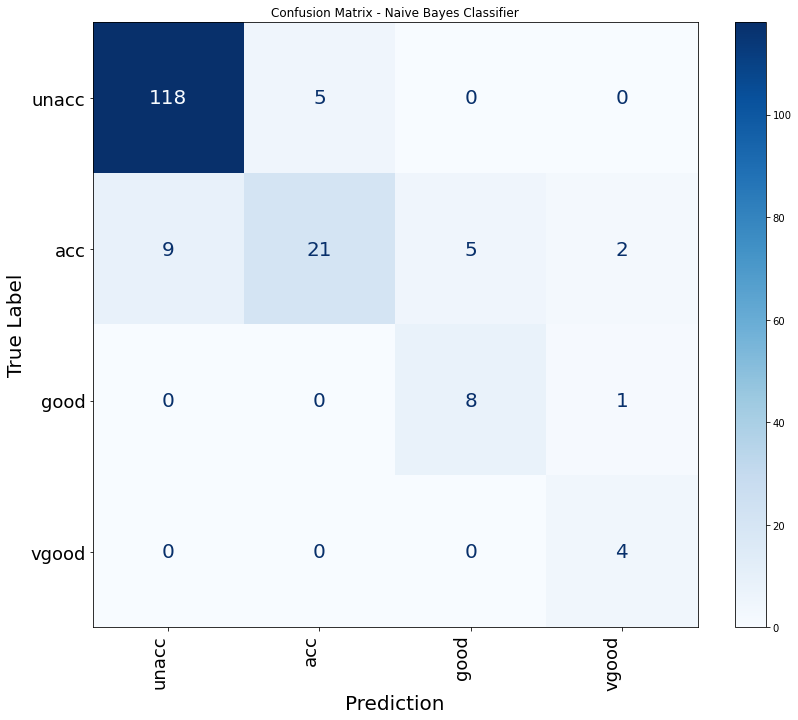
\includegraphics[scale=0.3]{images/NBCcm.png}}
  \caption{Confusion matrix of the Naive Bayes classifier} 
  \label{fig:NBCcm}
\end{figure}

\subsection{Results and Discussion}
The results of the NB classifier, as quantified by the metrics outlined in the previous section, are reported here. In this section of the project, the weighting factor of the minority classes are varied to investigate their influence on the classification performance on the minority classes. Since the minority classes have similar distribution in the dataset, the same weighting factor was applied to both classes.

\subsubsection{Classifier with unmodified prior probability}
When there was no weighting factor to boost the prior probability of the \lstinline{good} and \lstinline{vgood} classes, it was expected that the model would predominantly classify testing instances as either \lstinline{unacc} or \lstinline{acc}. This was evident when the prior probability of each minority class was below 0.04 compared to $p(unacc)=0.699$ and $p(acc)=0.223$. 

The overall accuracy of this classifier was 86.71\%. The confusion matrix of this unmodified classifier is shown in \autoref{fig:NBCcm_unmodified}. 

\begin{figure} [h]
  \centering{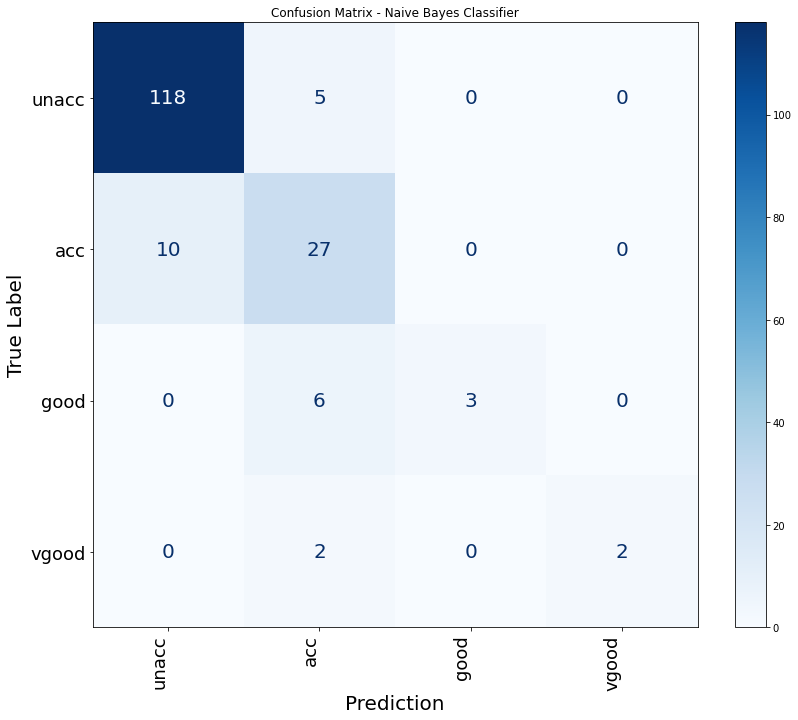
\includegraphics[scale=0.3]{images/NBCcm_unmodified.png}}
  \caption{Confusion matrix of the Naive Bayes classifier with unmodified prior probabilities} 
  \label{fig:NBCcm_unmodified}
\end{figure}


The other metrics of the model are included in \autoref{tab:nb_performance_unmodified}. As expected, the classifier exhibit outstanding precision and recall for the majority class. However, these quantities are significantly lower for the other three classes. This was the result of the prior probability discrepancy and lack of adequate training data in the minority classes.
\begin{table}[ht]
  \centering
  \caption{Performance Metrics of the Unmodified Naive Bayes classifier}
  \label{tab:nb_performance_unmodified}
  \begin{tabular}{||cccc||}
  \hline
  \textbf{ }        & \textbf{Precision}    & \textbf{Recall}   & \textbf{F1-score} \\
  \hline \hline
  unacc             & 0.92                  & 0.96              & 0.94\\ \hline
  acc               & 0.68                  & 0.73              & 0.73\\ \hline
  good              & 1.00                  & \hl{0.33}         & \hl{0.50}\\ \hline
  vgood             & 1.00                  & \hl{0.50}          & \hl{0.67}\\
  \hline
  \end{tabular}
\end{table}

\subsubsection{Classifier with a weighting factor of 5}
Compared to the unmodifed classifier, the accuracy improved to 87.86\% when incorporating a weighting factor of 5 on the prior probabilities of both the minority classes. \autoref{fig:NBCcm_5} shows the confusion matrix of this classifier, while the classifier recall, precision, and F1-score are included in \autoref{tab:nb_performance_5}. Compared to th previous confusion matrix, we observed a rightward shift in the prediction, where some \lstinline{acc} instances are classified as \lstinline{good} and \lstinline{vgood} and some instances previously misclassified as \lstinline{acc} are now correctly classified as the minority classes. Evident by \autoref{tab:nb_performance_5}, by increasing the importance of the minority class, the model achieved significantly better performance on the minority classes while only slightly reduce its previous performance in the \lstinline{acc} class.

\begin{figure} [h]
  \centering{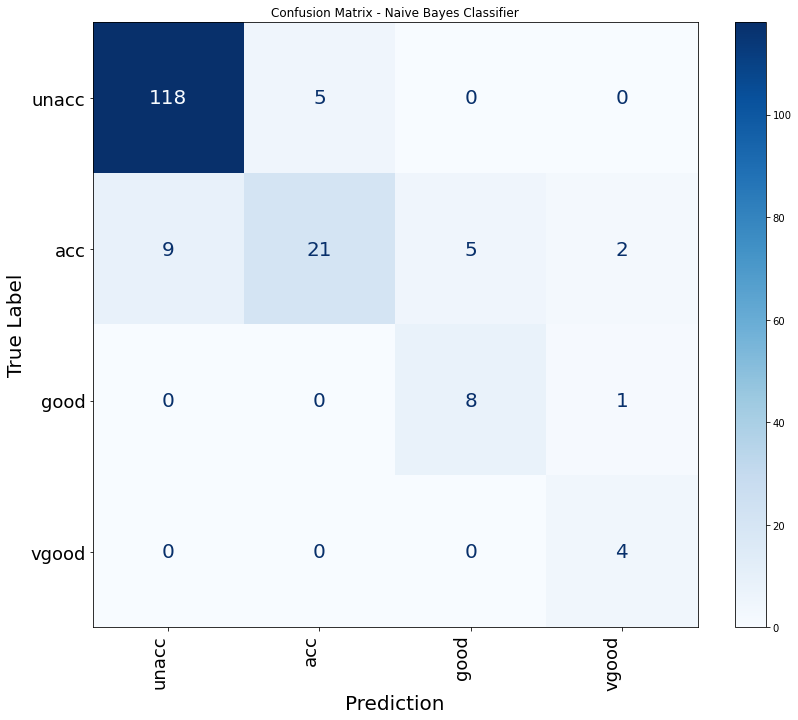
\includegraphics[scale=0.3]{images/NBCcm_10.png}}
  \caption{Confusion matrix of the Naive Bayes classifier with a weighting factor of 5} 
  \label{fig:NBCcm_5}
\end{figure}

\begin{table}[ht]
  \centering
  \caption{Performance Metrics of the Unmodified Naive Bayes classifier}
  \label{tab:nb_performance_5}
  \begin{tabular}{||cccc||}
  \hline
  \textbf{ }    & \textbf{Precision}    & \textbf{Recall}   & \textbf{F1-score} \\
  \hline \hline
  unacc         & 0.93                  & 0.96              & 0.94\\ \hline
  acc           & 0.81                  & 0.59              & 0.69\\ \hline
  good          & 0.67                  & \hl{0.89}         & \hl{0.76}\\ \hline
  vgood         & 0.57                  & \hl{1.00}         & \hl{0.73}\\
  \hline
  \end{tabular}
\end{table}


\subsubsection{Classifier with a weighting factor of 10}
The accuracy of the model was slightly improved to 87.28\% when a weighting factor of 10 was incorporated in the prior probability of both the \lstinline{good} and \lstinline{vgood} classes. The confusion matrix of the classifier is provided in \autoref{fig:NBCcm_10} while the classifier recall, precision, and F1-score are included in \autoref{tab:nb_performance_10}. In terms of the F1-score, this classifier had comparable performance for both the \lstinline{unacc} and \lstinline{acc} classes compared to the previous classifier with a slight decrease in performance for the \lstinline{good} class

\begin{figure} [h]
  \centering{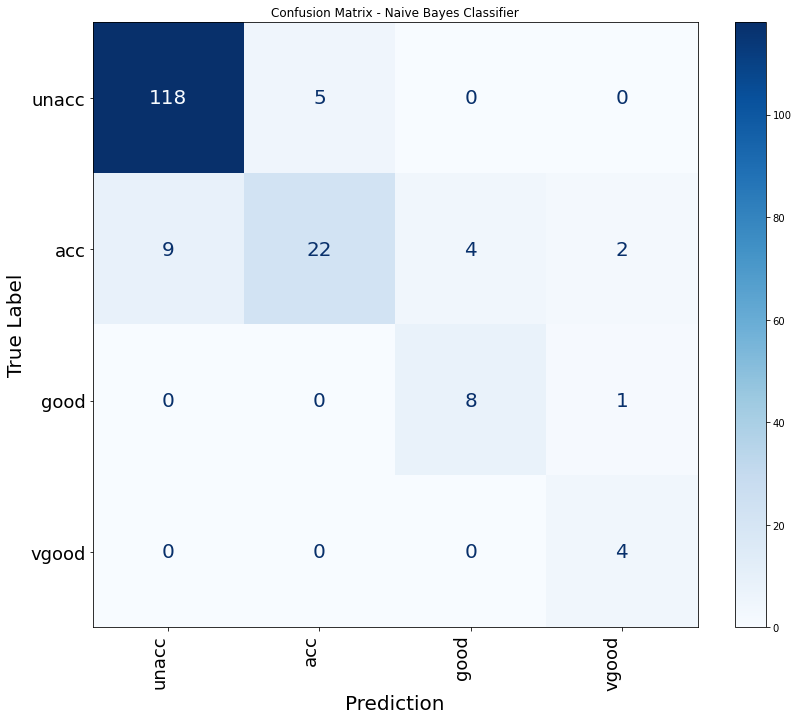
\includegraphics[scale=0.3]{images/NBCcm_5.png}}
  \caption{Confusion matrix of the Naive Bayes classifier with a weighting factor of 10} 
  \label{fig:NBCcm_10}
\end{figure}


\begin{table}[ht]
  \centering
  \caption{Performance Metrics of the Unmodified Naive Bayes classifier}
  \label{tab:nb_performance_10}
  \begin{tabular}{||cccc||}
  \hline
  \textbf{ } & \textbf{Precision} & \textbf{Recall} & \textbf{F1-score} \\
  \hline \hline
  unacc & 0.93 & 0.96 & 0.94\\ \hline
  acc  & 0.81 & 0.57 & 0.67\\ \hline
  good & 0.62 & \hl{0.89} & \hl{0.73}\\ \hline
  vgood & 0.57 & \hl{1.00} & \hl{0.73}\\ \hline
  \end{tabular}
\end{table}

\subsection{Classifier with more prior probability adjustments} 
It was determined that there was no further imporvement in the model performance by further scaling the prior probability of the minority classes. At this point, more data is needed to fine tune and improve the performance of the model, especially for classifying the minority classes. Another methods was to manually fine tune the weighting factors of the \lstinline{acc} class. To test this, the weighting factors for the minority classes were fixed while the weighting factor of \lstinline{acc} was increased. The minority class weighting factor was fixed at 5 since this gave the best performance from previous sections, and the weighting factor of \lstinline{acc} was initialized at 1.25 and later increased to 1.5. The reason behind the conservative factor stems from the concern of misclassifying unacceptable cars as acceptable.

The accuracy was 87.86\% for the model with the 1.25 weighting factor and it was 86.71\% for the models with the 1.5 weighting factor. The confusion matrices of these classifiers are shown in \autoref{fig:NBCcm_acc_class_weight_factor} and the performance metrics are summarized in \autoref{tab:nb_performance_1.25_5_5}.


\begin{figure}[ht]
  % typeset
  \centering
  \subcaptionbox{\label{subfig:NBCcm_1.25_5_5}}{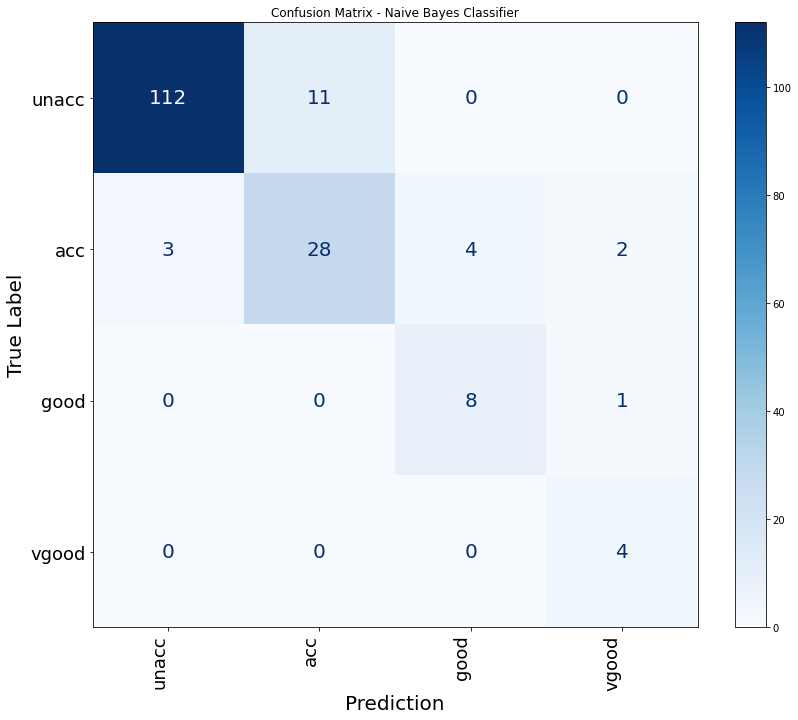
\includegraphics[width=0.48\textwidth]{images/NBCcm_1.25_5_5.png}}
  \subcaptionbox{\label{subfig:NBCcm_1.5_5_5}}{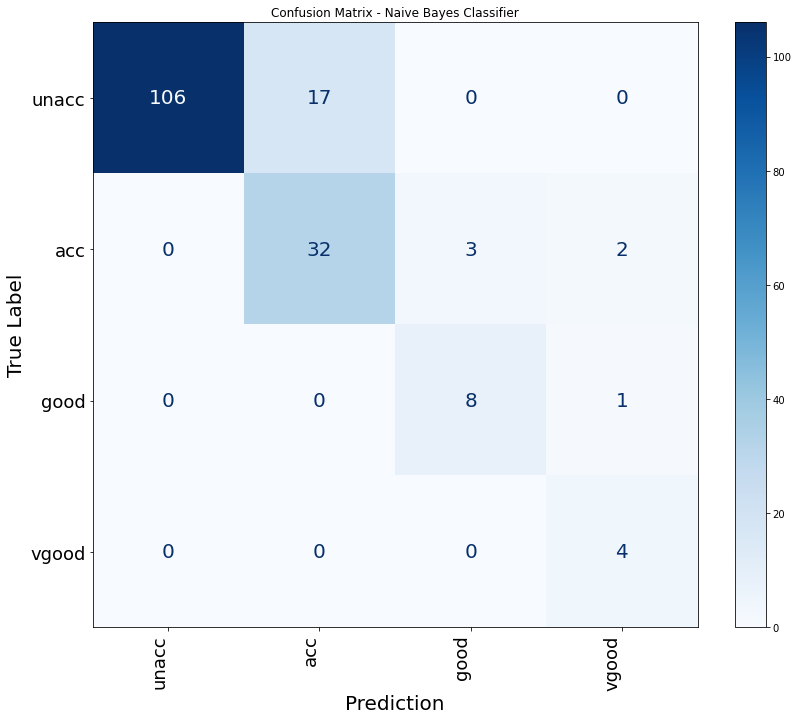
\includegraphics[width=0.48\textwidth]{images/NBCcm_1.5_5_5.png}}
  \caption{Confusion matrix of the Naive Bayes classifier with a weighting factor of 5 for the minority classes and a weigting factor of 1.25 (left) and 1.5 (right) for the \lstinline{acc} class}
  \label{fig:NBCcm_acc_class_weight_factor}
\end{figure}

\begin{table}[ht]
  \centering
  \caption{Performance Metrics of the Naive Bayes classifier with mixed weighting factors}
  \label{tab:nb_performance_1.25_5_5}
  \begin{tabular}{||c | c c c | c c c||}

  \hline
  \centering
  \multirow{2}{*}{Class}    & \multicolumn{3}{c|}{Model 1 - Factor of 1.25}                     & \multicolumn{3}{c||}{Model 2 - Factor of 1.50} \\\cline{2-7} 
                            & \textbf{Precision}  & \textbf{Recall}   & \textbf{F1-score}       & \textbf{Precision}  & \textbf{Recall}   & \textbf{F1-score}\\
  \hline \hline
  unacc                     & 0.97                & 0.91              & 0.94                    & 1.00                & 0.86              & 0.93\\ \hline
  acc                       & 0.72                & 0.76              & 0.74                    & 0.65                & 0.86              & 0.74\\ \hline
  good                      & 0.67                & \hl{0.89}         & \hl{0.76}               & 0.73                & \hl{0.89}         & \hl{0.80}\\ \hline
  vgood                     & 0.57                & \hl{1.00}         & \hl{0.73}               & 0.57                & \hl{1.00}         & \hl{0.73}\\ \hline
  \end{tabular}
\end{table}


It was found that by increasing this weighting factor to 1.25 and 1.5 achieve better F1-score for the \lstinline{acc} class and the minority classes. However, from the confusion matrix of these classifiers, more unacc instances were classified as acceptable. This was reflected in the decrease in the recall metric of the \lstinline{unacc} class. Depending on the severity of this misclassification in the real-world scenario (i.e., passing an unacceptable car with low safety and high buying price as acceptable), this improvement is not desireable.

\section{ANN Experiment with the MNIST handwritten digit dataset}
In this section of the project report, the team reports the experimentation detail and results from implementing two ANN methods on the task of MNIST handwritten digit recognition
\subsection{Dataset Details}
The dataset of handwritten digits used to train and test the CNN was provided by MNIST and contained 60,000 training examples and 10,000 test examples. The examples were already split as described when acquired. \autoref{fig:mnist-examples} contains 9 images randomly sampled from the 60,000 training instances and demonstrates what the CNN will be learning on and trying to classify.

\begin{figure}[h]
    \centering
    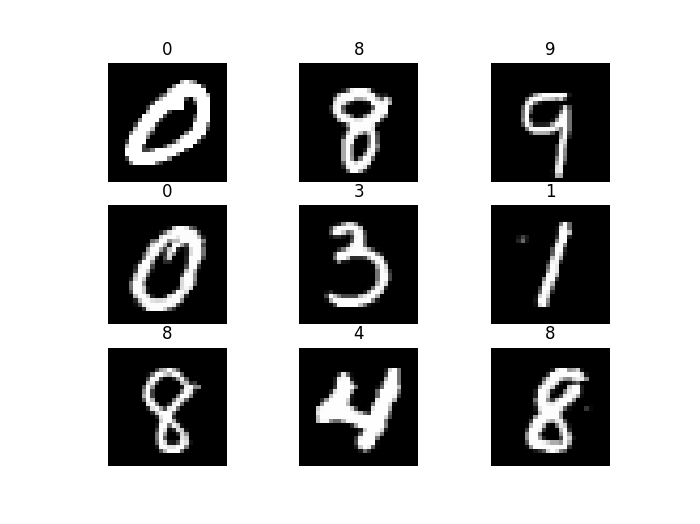
\includegraphics[scale=0.5]{images/mnist-examples.png}
    \caption{Nine randomly chosen examples from the MNIST handwritten digit dataset.}
    \label{fig:mnist-examples}
\end{figure}

Among the provided dataset were 10 unique classes, the digits ranging from 0 to 9. The distribution of these classes among the training dataset can be seen in Figure~\ref{fig:mnist-class-dist}. Due to the nearly uniform distribution shown in Figure~\ref{fig:mnist-class-dist}, no pre-processing of the data was performed.

\begin{figure}[h]
    \centering
    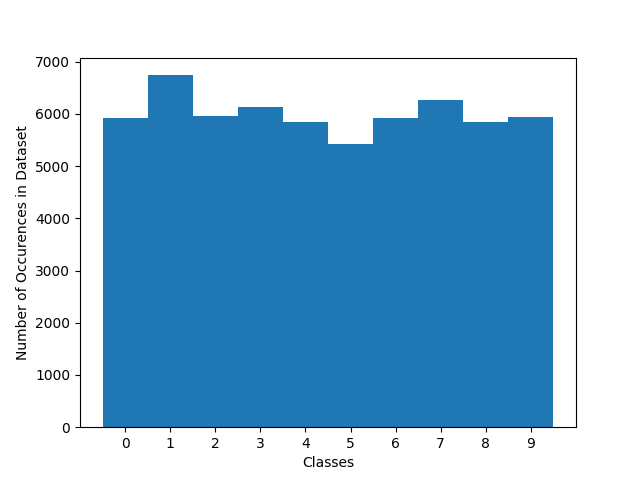
\includegraphics[scale=0.5]{images/mnist-class-dist.png}
    \caption{Distribution of classes within the MNIST handwritten digit dataset.}
    \label{fig:mnist-class-dist}
\end{figure}

\subsection{Fully-Connected Feedforward Neural Network}
In the FNN implementation of the handwritten digit recognition task, the TensorFlow Keras library was used extensively to formulate and train the model. There are several hyperparameters of interest that have a significant impact on the model performance. In this experiment, the team investigated the effect of the following four hyperparameters:

\begin{enumerate}
    \item \textbf{Model structure} - this governs both the depth and the width of the FNN. The depth of the FNN is the number of hidden layer, while the width of the network is the number of neurons in each layer. Theoretically, wider and deeper networks benefits from learning more complex latent features in the input, thus are expected to have higher performance. There are four model structures tested in this experiment
    \begin{itemize}
        \item a 2-layer model with 64 and 32 neurons,
        \item a 2-layer model with 32 and 16 neurons,
        \item a 3-layer model with 64, 32, and 16 neurons, and
        \item a 3-layer model with 32, 16, and 8 neurons.
    \end{itemize}
    \item \textbf{Learning Rate} - this governs the speed of parameter optima convergence. Theoretically, a lower learning rate improbe the model training stability since the parameters are adjusted at a lower rate at every update. However, the model will also take a longer time to train. To investigate the effect of the learning rate on the model performance, learning rates of 0.001, 0.0005, and 0.0001 were tested.
    \item \textbf{Epoch} - epochs governs the number of time that the entire training dataset used for training the model and updating the paramaters. The model parameters have the chance to improve and reach the optima with a higher number of epochs. However, the model can also overfit if it adapts to the specific features present in the training data but is not representative of validation or testing data. In this experiment, epoch sizes of 10, 25, and 50 were investigated.
    \item \textbf{Activation Function} - The selection of activation function must consider different advantages and disadvantages of each function. For example, the sigmoid function is prone to the vanishing gradient problem for deep networks, thus ealier layers cannot effectively adjust in response to the loss function value. ReLU activation was introduced as a better alternative to tackle this vanishing gradient problem. The team investigated the effect of these activation functions on the model performance
\end{enumerate}

\subsubsection{Implementation Detail of FNNs}
The construction of the FNN models followed a typical workflow of data import and exploration, model construction, model training, and model evaluation. In this project, this pipeline was done once for one model before being scaled up for a hyperparameter grid search.

\begin{enumerate}
    \item \textbf{Data import and exploration} - The Kaggle data was downloaded using the KaggleHub API and moved to within the project repository for easy access. Since the data file has a non-standard file type, the team utilized the \lstinline{MnistDataLoader()} and \lstinline{show_image()} classes provided with the dataset. Visualization of random samples from the training dataset were shown in \autoref{fig:mnist-examples}. The data was loaded into train and test feature and label sets using the data loader object. The number of instance in each set and the structure of the sets were investigated. Furthermore, the training data was further split into a train set and a validation set, so that the test set would be purely for testing and not access during the training process.
    
    Since there is a high number of models in the search space, the models will be trained on a GPU to accelerate the training process. However, the team had previously experienced some training difficulties on a memory-constrained GPU due to the training implementation of TensorFlow. To avoid the memory constrain problem, a DataGenerator() class was defined to send training data to the model in batches. 
    \item \textbf{ANN Model Construction Function} - To easily construct any model when given the hyperparameter configuration, a function called \lstinline{build_ann_model()} for building ANN models was created. The function creates a Keras sequential model that starts with a flatten layer to flatten the 2D input into a 1D tensor. This layer is then followed by alternate Dense and BatchNormalization layers. The activation function of the dense layer is by default ReLU but can be defined otherwise. The number of layers and the number of neurons in each layer is defined by the input argument \lstinline{layer_widths}, which is a list of neurons in each hidden layer. The output layer is appended to the sequential model as a Dense layer with the number of neuron being the number of output classes. The activation function of this dense layer is always the softmax function. Within this function, the model is compiled with a learning rate, a loss function, and tracked metrics as defined by the corresponding input arguments.
    
    \item \textbf{Testing with one ANN model construction} - This function was first tested by building and training one model. A corresponding directory with the hyperparameter configuration was created to store the the hyperparameters and training performance. The \lstinline{plot_performance()} helper function was defined to visualize the model training history. Aside from plotting the training and testing loss and tracked metrics, the model was later modified such that the plots are saved in a specified directory. This helps keep a record of training performance for different model with different hyperparameter configurations.

    \item \textbf{Grid Search Model Training} - In this section, the parameter grid previously specified were setup such that the algorithm iterate through each hyperparameter configuration combination. In each iteraction, the algorithm
    \begin{itemize}
        \itemsep=-5pt
        \item creates a new directory corresponding to the training time and the current hyperparameter configuration, 
        \item builds the model using the \lstinline{build_ann_model()} function defined above, 
        \item saves the training parameters in a \lstinline{training_params} dictionary, 
        \item saves the model\ summary/structure into a \lstinline{model_summary.json} file, 
        \item trains the model and save the training time and final training result in a \lstinline{training_results} dictionary, 
        \item stores the training parameters and final training results into a \lstinline{params_results.json} file, 
        \item saves the model for future inference and testing, and 
        \item plots the model training history using the  and save the figure in the directory
    \end{itemize}
    
    \item \textbf{Model Training Performance Visualization} - After all the models were trained and stored in the corresponding folder in the \lstinline{ann_model_results} directory, the model hyperparameters and training results can be extracted from the JSON files and stored in a \lstinline{results_df} dataframe. In this section, the team investigated the top 10 hyperparameter configurations that resulted in the highest training accuracy and validation accuracy. These models are summarized in \autoref{tab:ann_performance_top10_training_accuracy} and \autoref{tab:ann_performance_top10_validation_accuracy}. Furthermore, to investigate the effect of each hyperparameter on a macro level, the resulting data frame was grouped according to each hyperparameter and a box plot was drawn to capture the overall performance for each value of the hyperparameter. These results are included in section \ref{ann_model_result_hyperparameter}
\end{enumerate}

\begin{table}[ht]
    \centering
    \caption{Training performance of the 10 models with the highest training accuracy}
    \label{tab:ann_performance_top10_training_accuracy}
    \begin{tabular}{|| c c c c | c c c c ||}
  
    \hline
    \centering
    \textbf{Structure}  &\textbf{learning\_rate} &\textbf{epochs}    &\textbf{activation}    & \textbf{train\_loss}   &\textbf{train\_acc} &\textbf{val\_loss}  &\textbf{val\_acc} \\
    \hline \hline
    [64,32]             & 0.0001                & 50                & relu                  & 0.000927              & 1.000000          &0.229352           & 0.966833 \\ 
    \hline
    [64,32,16]          & 0.0005                & 50                & relu                  & 0.003082              & 0.999146          &0.168138           & 0.973083 \\ 
    \hline
    [64,32,16]          & 0.0001                & 50                & relu                  & 0.005420              & 0.998521          &0.229432           & 0.961750 \\ 
    \hline
    [64,32]             & 0.0005                & 50                & relu                  & 0.004767              & 0.998396          &0.175682           & 0.970667 \\ 
    \hline
    [64,32]             & 0.0010                & 50                & relu                  & 0.005936              & 0.998208          &0.188590           & 0.970664 \\ 
    \hline
    [64,32]             & 0.0001                & 25                & relu                  & 0.016039              & 0.998042          &0.125761           & 0.967917 \\ 
    \hline
    [64,32]             & 0.0005                & 25                & relu                  & 0.007371              & 0.998021          &0.166564           & 0.966417 \\ 
    \hline
    [32,16]             & 0.0005                & 50                & relu                  & 0.009465              & 0.997667          &0.254109           & 0.957000 \\ 
    \hline
    [64,32,16]          & 0.0010                & 50                & relu                  & 0.007377              & 0.997604          &0.188418           & 0.970417 \\ 
    \hline
    [64,32]             & 0.0010                & 25                & relu                  & 0.008554              & 0.997333          &0.158781           & 0.971250 \\ 
    \hline
    \end{tabular}
\end{table}

\begin{table}[ht]
    \centering
    \caption{Training performance of the 10 models with the highest validation accuracy}
    \label{tab:ann_performance_top10_validation_accuracy}
    \begin{tabular}{|| c c c c | c c c c ||}
  
    \hline
    \centering
    \textbf{Structure}  &\textbf{learning\_rate} &\textbf{epochs}    &\textbf{activation}    & \textbf{train\_loss}   &\textbf{train\_acc} &\textbf{val\_loss}  &\textbf{val\_acc} \\
    \hline \hline
    [64,32,16]          & 0.0005                & 50                & relu                  & 0.003082              & 0.999146          &0.168138           & 0.973083 \\ 
    \hline
    [64,32,16]          & 0.0005                & 25                & relu                  & 0.010872              & 0.996625          &0.143203           & 0.972917 \\ 
    \hline
    [64,32,16]          & 0.0010                & 25                & relu                  & 0.013520              & 0.995625          &0.124847           & 0.972833 \\ 
    \hline
    [64,32]             & 0.0010                & 25                & relu                  & 0.008554              & 0.997333          &0.158781           & 0.971250 \\ 
    \hline
    [64,32]             & 0.0005                & 50                & relu                  & 0.004767              & 0.998396          &0.175682           & 0.970667 \\ 
    \hline
    [64,32]             & 0.0010                & 50                & relu                  & 0.005936              & 0.998208          &0.188590           & 0.970667 \\ 
    \hline
    [64,32,16]          & 0.0010                & 50                & relu                  & 0.007377              & 0.997604          &0.188418           & 0.970417 \\ 
    \hline
    [64,32]             & 0.0010                & 10                & relu                  & 0.033115              & 0.989792          &0.109751           & 0.970333 \\ 
    \hline
    [64,32]             & 0.0005                & 10                & relu                  & 0.031812              & 0.990896          &0.110450           & 0.968917 \\ 
    \hline
    [64,32]             & 0.0001                & 25                & relu                  & 0.016039              & 0.998042          &0.125761           & 0.967917 \\ 
    \hline
    \end{tabular}
\end{table}

\subsubsection{Results of Training and Validation Performance} \label{ann_model_result_hyperparameter}
\textbf{Effects of the model structure}

\begin{figure} [htbp]
    \centering{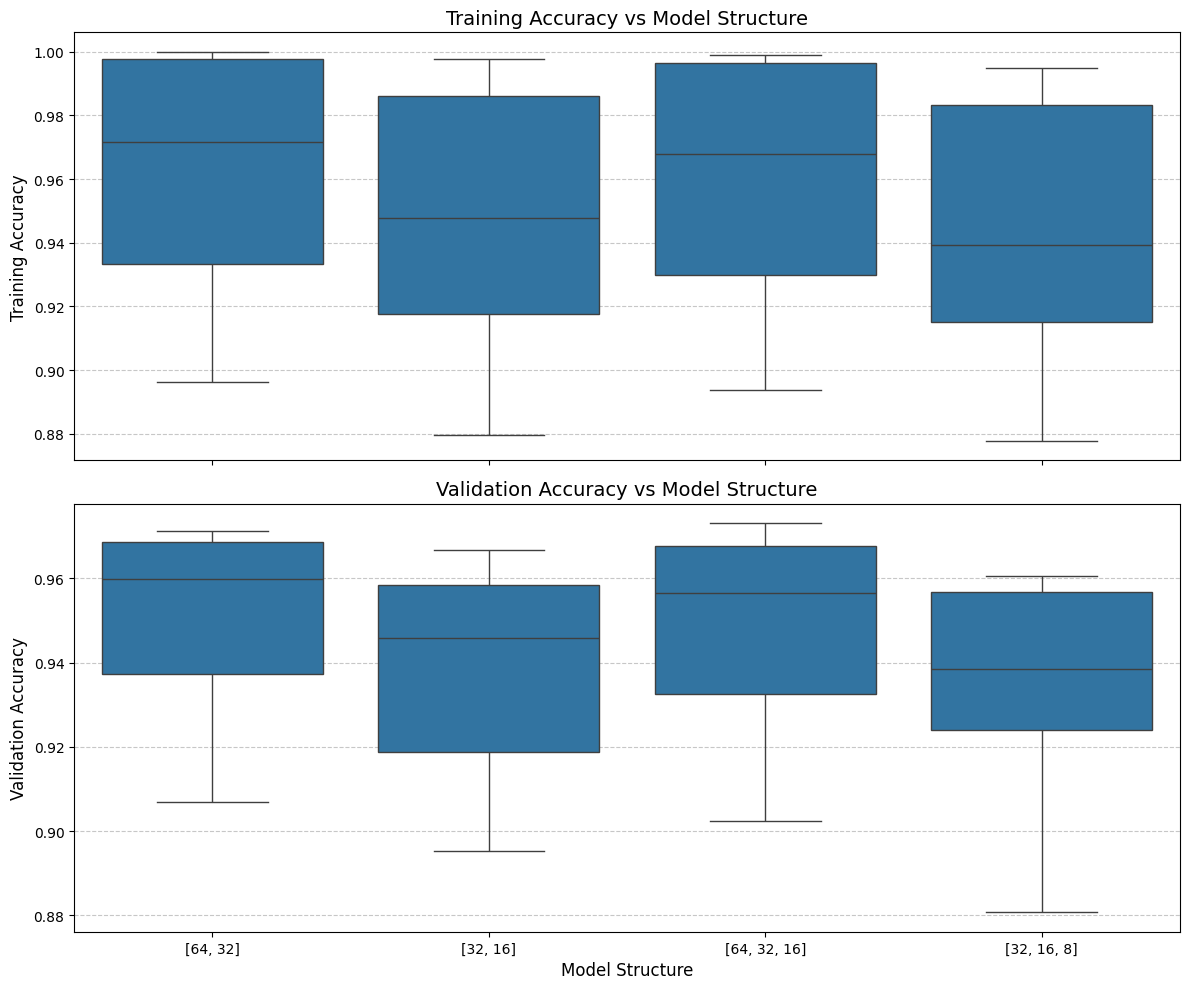
\includegraphics[width=0.8\linewidth]{images/mnist_ann_result_modelstructure.png}}
    \caption{The effect of the model structure on the training and validation accuracy} 
    \label{fig:mnist_ann_result_modelstructure}
\end{figure}

\textbf{Effects of the learning rate}

\begin{figure} [htbp]
    \centering{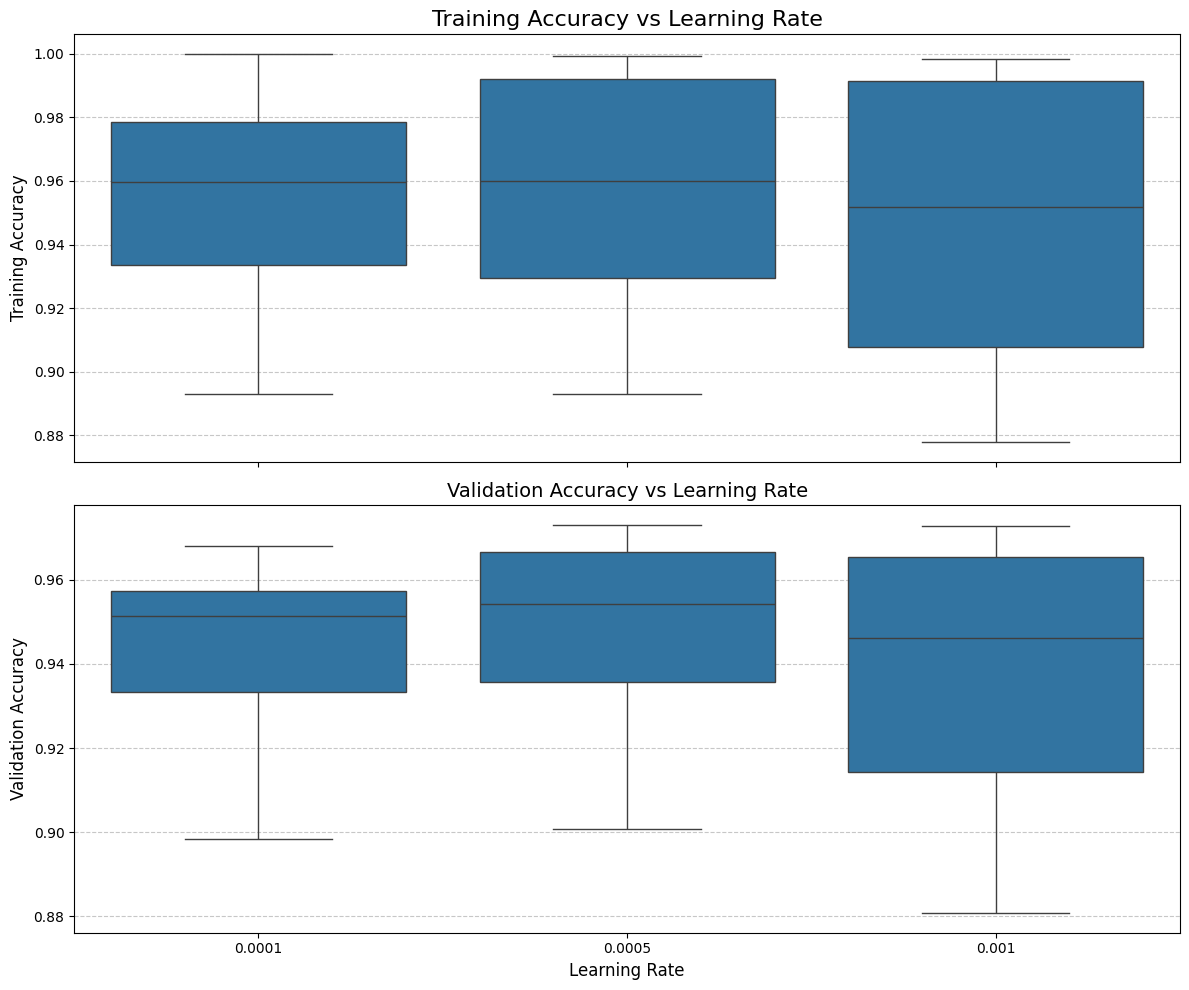
\includegraphics[width=0.8\linewidth]{images/mnist_ann_result_learningrate.png}}
    \caption{The effect of the learning rate on the training and validation accuracy} 
    \label{fig:mnist_ann_result_learningrate}
\end{figure}

\textbf{Effects of the epoch size}


\begin{figure} [htbp]
    \centering{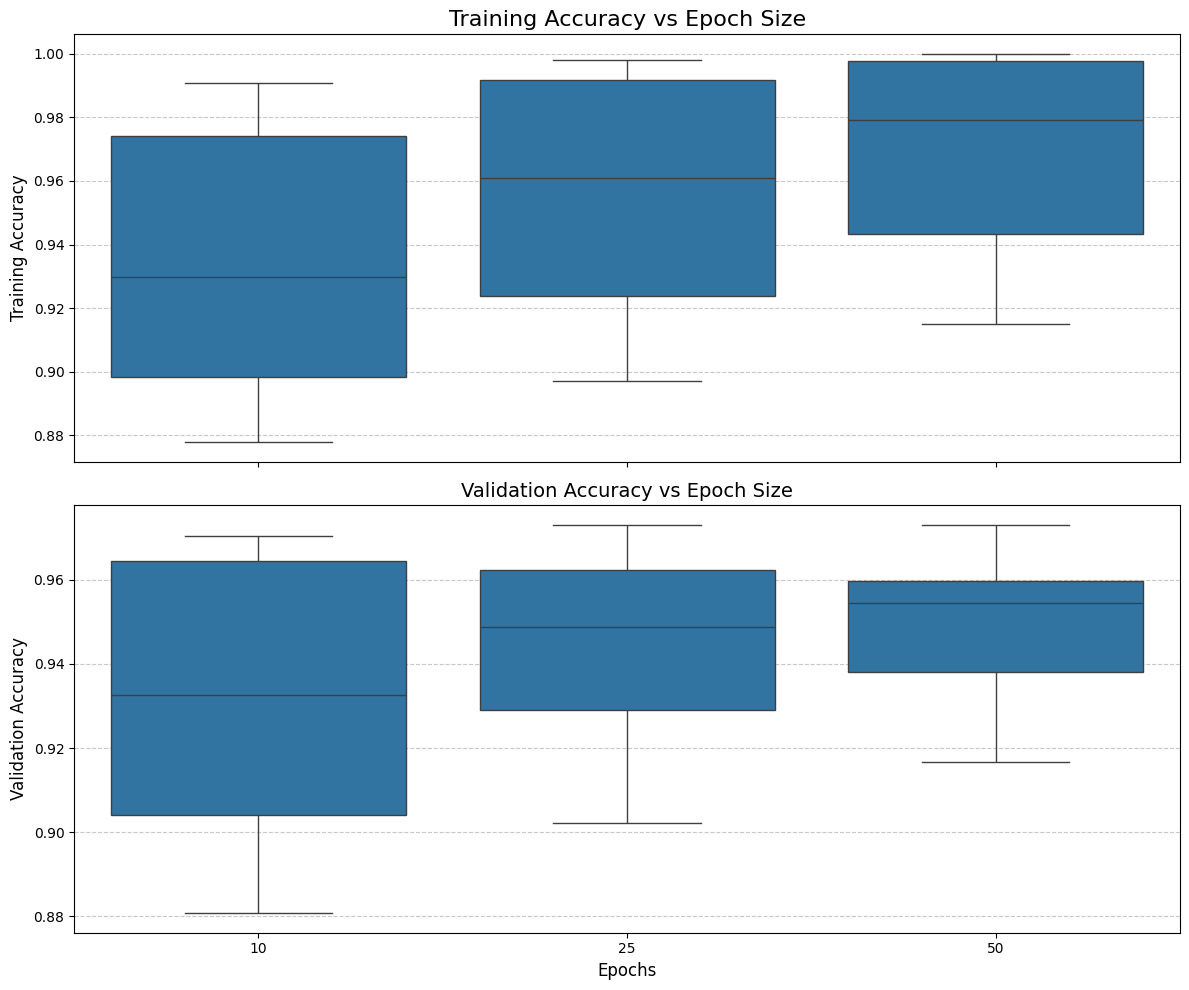
\includegraphics[width=0.8\linewidth]{images/mnist_ann_result_epoch.png}}
    \caption{The effect of the epoch size on the training and validation accuracy} 
    \label{fig:mnist_ann_result_epoch}
\end{figure}

\textbf{Effects of the activation function}


\begin{figure} [htbp]
    \centering{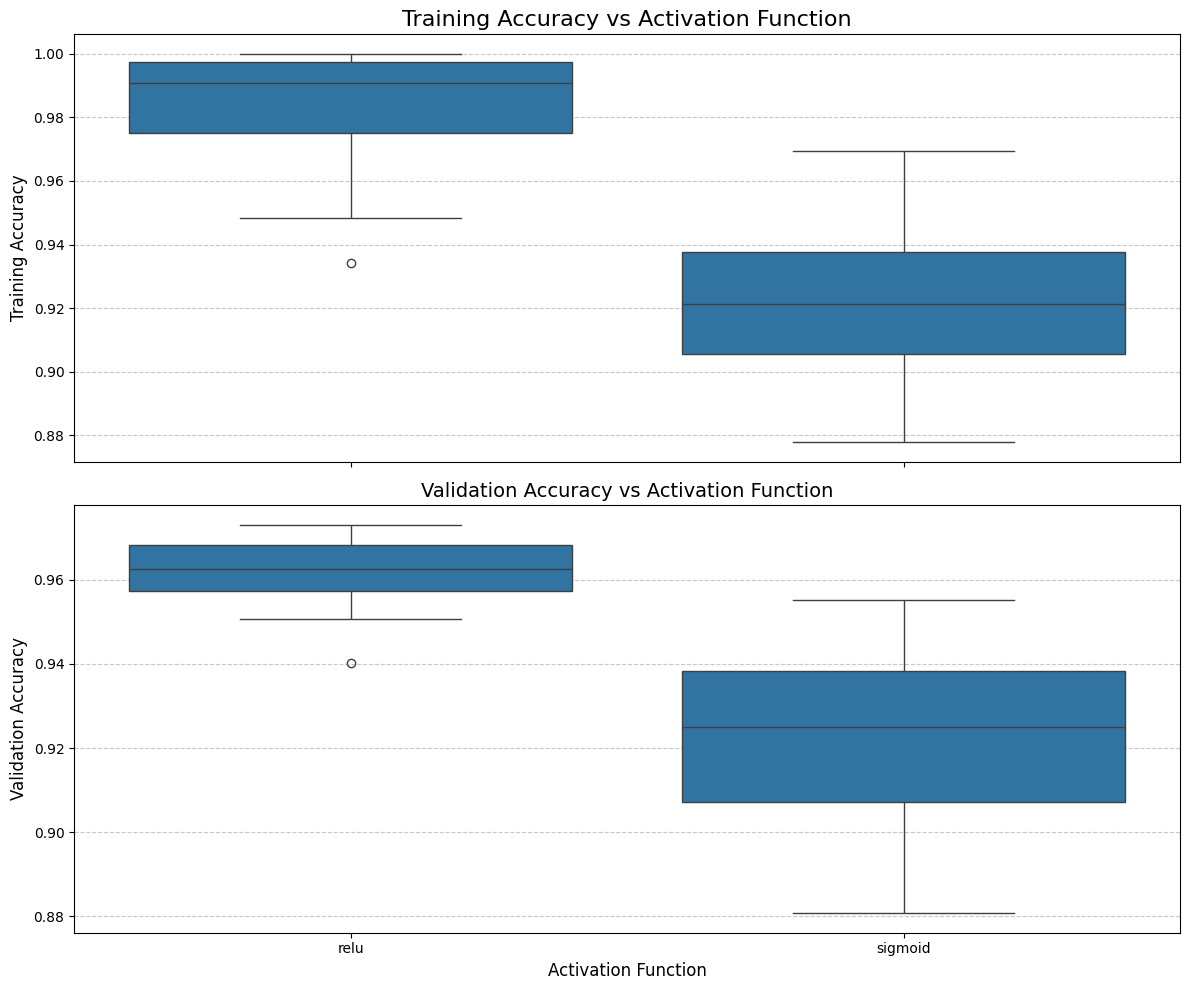
\includegraphics[width=0.8\linewidth]{images/mnist_ann_result_activation.png}}
    \caption{The effect of the activation function on the training and validation accuracy} 
    \label{fig:mnist_ann_result_activation}
\end{figure}

\newpage

\section{Convolutional Neural Network}
A convolutional neural network (CNN) was successfully created using existing machine learning libraries to train on and classify handwritten digits using the MNIST dataset. The structure and several training parameters of this CNN were varied to evaluate the effect these parameters have on the performance of the model. This CNN was implemented using the \textit{TensorFlow} Python library, alongside its high-level API \textit{Keras}. These libraries were chosen based on their ease-of-use for implementing a CNN that can easily have its structure re-arranged in code. 

\subsection{Testing Different CNN Structures}

As was previously mentioned, several aspects of the structure of the CNN were varied and tested to evaluate their effect on the performance of the model. The following structural components of the CNN were varied and compared:
\begin{enumerate}
    \item The number of filters of each convolutional layer in the CNN.
    \item The number of layers in the CNN.
    \item The addition of a drop-out layer in the CNN, tested with different drop-out rates.
    \item The addition of batch-normalization layers after each convolutional layer in the CNN.
    \item Using average pooling layers vs. max pooling layers. 
\end{enumerate}
In addition to this, several results of the above modifications to the structure of the CNN were compared to a control CNN model with the following default structural attributes:
\begin{itemize}
    \item Number of layers: 3
    \item Number of filters: 32
    \item No drop-out layers.
    \item No batch normalization layers.
    \item Use of max pooling for pooling layers.
\end{itemize}
The performance curve of this control CNN model can be seen in Figure~\ref{fig:control-cnn}. Please note that the number of layers referenced above represents the number of convolutional and pooling layer pairs, and does not include the fully-connected feed-forward network used for classification after these layers.

\begin{figure}[h]
    \centering
    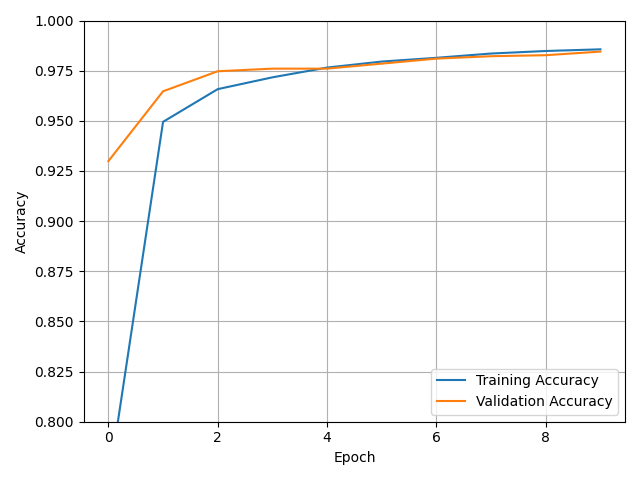
\includegraphics[scale=0.5]{images/control-cnn.png}
    \caption{Performance of control CNN with default structure.}
    \label{fig:control-cnn}
\end{figure}

\subsubsection{Number of Layers and Filters}

The results of training the CNN model with 1, 2, and 3 layers, as well as training the model with 16, 32, and 64 filters, can be seen in Figure~\ref{fig:layers-filters}. The results in Figure~\ref{fig:layers-filters} demonstrates how increasing the number of filters can actually lead to over-fitting in the CNN. The maximum training and validation accuracy after 10 epochs for the 16 filter and 32 filter models stay relatively close together. However, for the 64 filter case, the accuracies actually diverge with the validation accuracy being less than the training accuracy. Conversely, Figure~\ref{fig:layers-filters} also demonstrates how increasing the number of layers in the CNN model actually reduces the effect of over-fitting.

\begin{figure}[h]
    \centering
    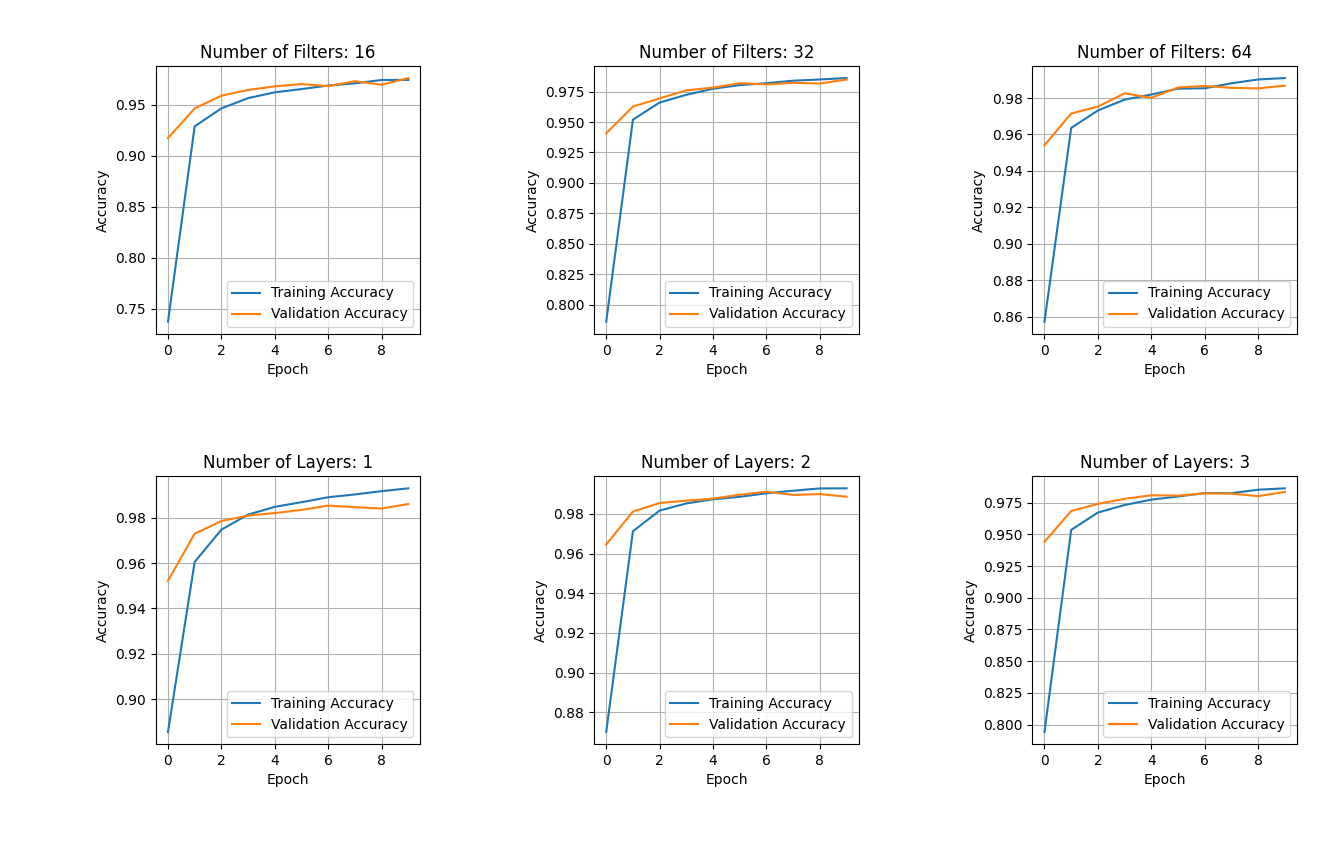
\includegraphics[scale=0.45]{images/n-layers-n-filters-cnn.png}
    \caption{Performance of training the CNN model with different number of layers and filters.}
    \label{fig:layers-filters}
\end{figure}

\subsubsection{Addition of Drop-Out Layers}

The results of training the CNN model with the addition of drop-out layers with varying drop-out rates after each convolutional layer can be seen in Figure~\ref{fig:drop-out}. These models were trained with 3 total convolutional and pooling layer pairs, thus 3 total drop-out layers. As expected, the results shown in Figure~\ref{fig:drop-out} demonstrate reduced overfitting of the model as the drop-out rate increases, at the cost of training accuracy. It's clear from the results of the control model in Figure~\ref{fig:control-cnn} that over-fitting isn't a particularly big problem for our model, as such the use of drop-out layers is not necessary. 

\begin{figure}[h]
    \centering
    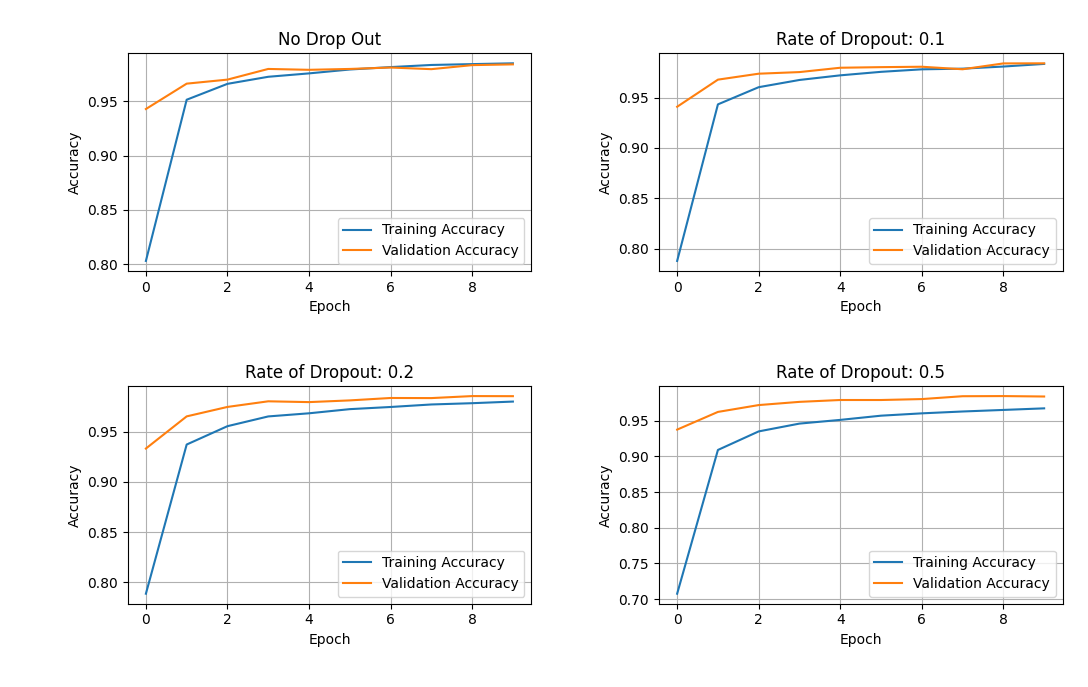
\includegraphics[scale=0.5]{images/drop-out-cnn.png}
    \caption{Performance of training the CNN model with drop-out layers of varying drop-out rates.}
    \label{fig:drop-out}
\end{figure}

\subsubsection{Addition of Batch Normalization Layers}

The results of training the CNN model with the addition of batch normalization layers after each convolutional layer can be seen in Figure~\ref{fig:batch-norm}. These results clearly demonstrate how batch normalization can be used as an effective regularizer. The maximum training and validation accuracies after 10 epochs diverge considerably when batch normalization is used, with the validation accuracy being the strongest, compared to the control model. This shows reduced over-fitting in the model.

\begin{figure}[h]
    \centering
    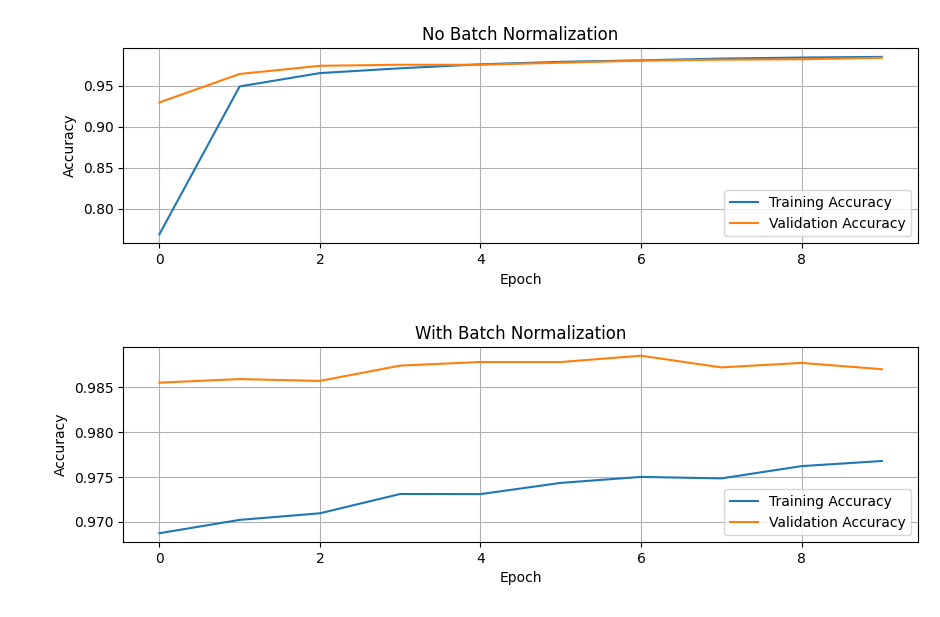
\includegraphics[scale=0.5]{images/batch-norm-cnn.png}
    \caption{Performance of training the CNN model with batch normalization layers.}
    \label{fig:batch-norm}
\end{figure}

\subsubsection{Max Pooling vs. Average Pooling}

The results of training the CNN model with both max pooling and average pooling layers can be seen in Figure~\ref{fig:pooling}. Pooling layers directly follow convolutional layers to down-sample the feature map output from these layers. How they accomplish this is either through a max operation or average operation over a defined window of the feature map output from the convolutional layer. From Figure~\ref{fig:pooling} it can be seen that using average pooling significantly reduces the training accuracy of the model, however the validation accuracy stays consistent with the model that used max pooling. It appears that due to the simplicity of this task, the difference between using max pooling vs. average pooling is not as significant. However, this may not be the case in other problems that require training a CNN model.

\begin{figure}[h]
    \centering
    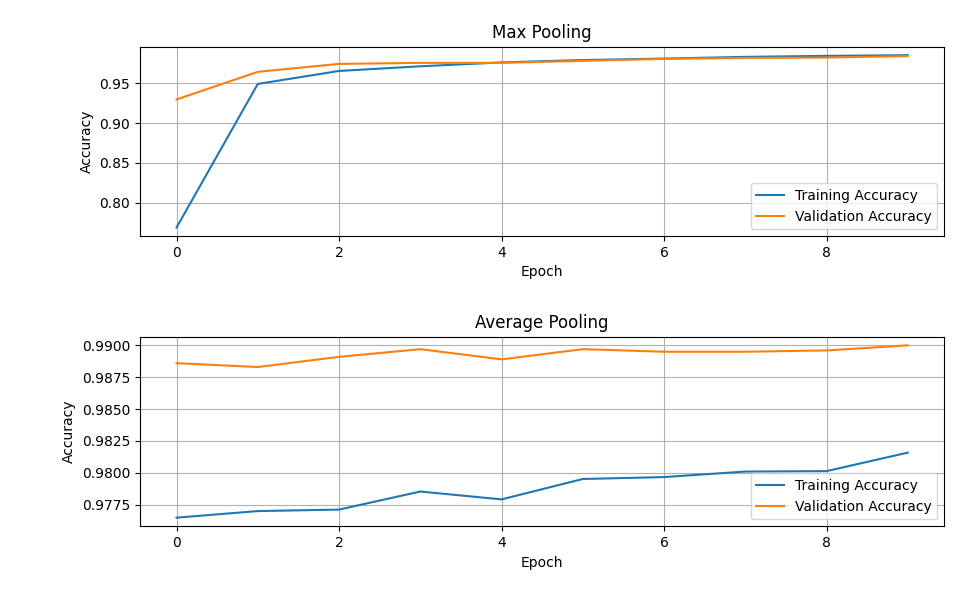
\includegraphics[scale=0.5]{images/max-avg-pooling-cnn.png}
    \caption{Performance of training the CNN model with both max pooling and average pooling layers.}
    \label{fig:pooling}
\end{figure}

\subsection{Testing Different Training Parameters}
In addition to experimenting on the structure of the CNN model to evaluate its performance, two training parameters were also varied to evaluate their effect on the performance of the model. These training parameters were:
\begin{enumerate}
    \item The learning rate of the model using a stochastic gradient descent optimizer.
    \item The batch size, or the number of samples per gradient update.
\end{enumerate}
The result of varying these trainig parameters on the performance of a CNN with 3 layers can be seen in Figure~\ref{fig:training-params}.

\begin{figure}[h]
    \centering
    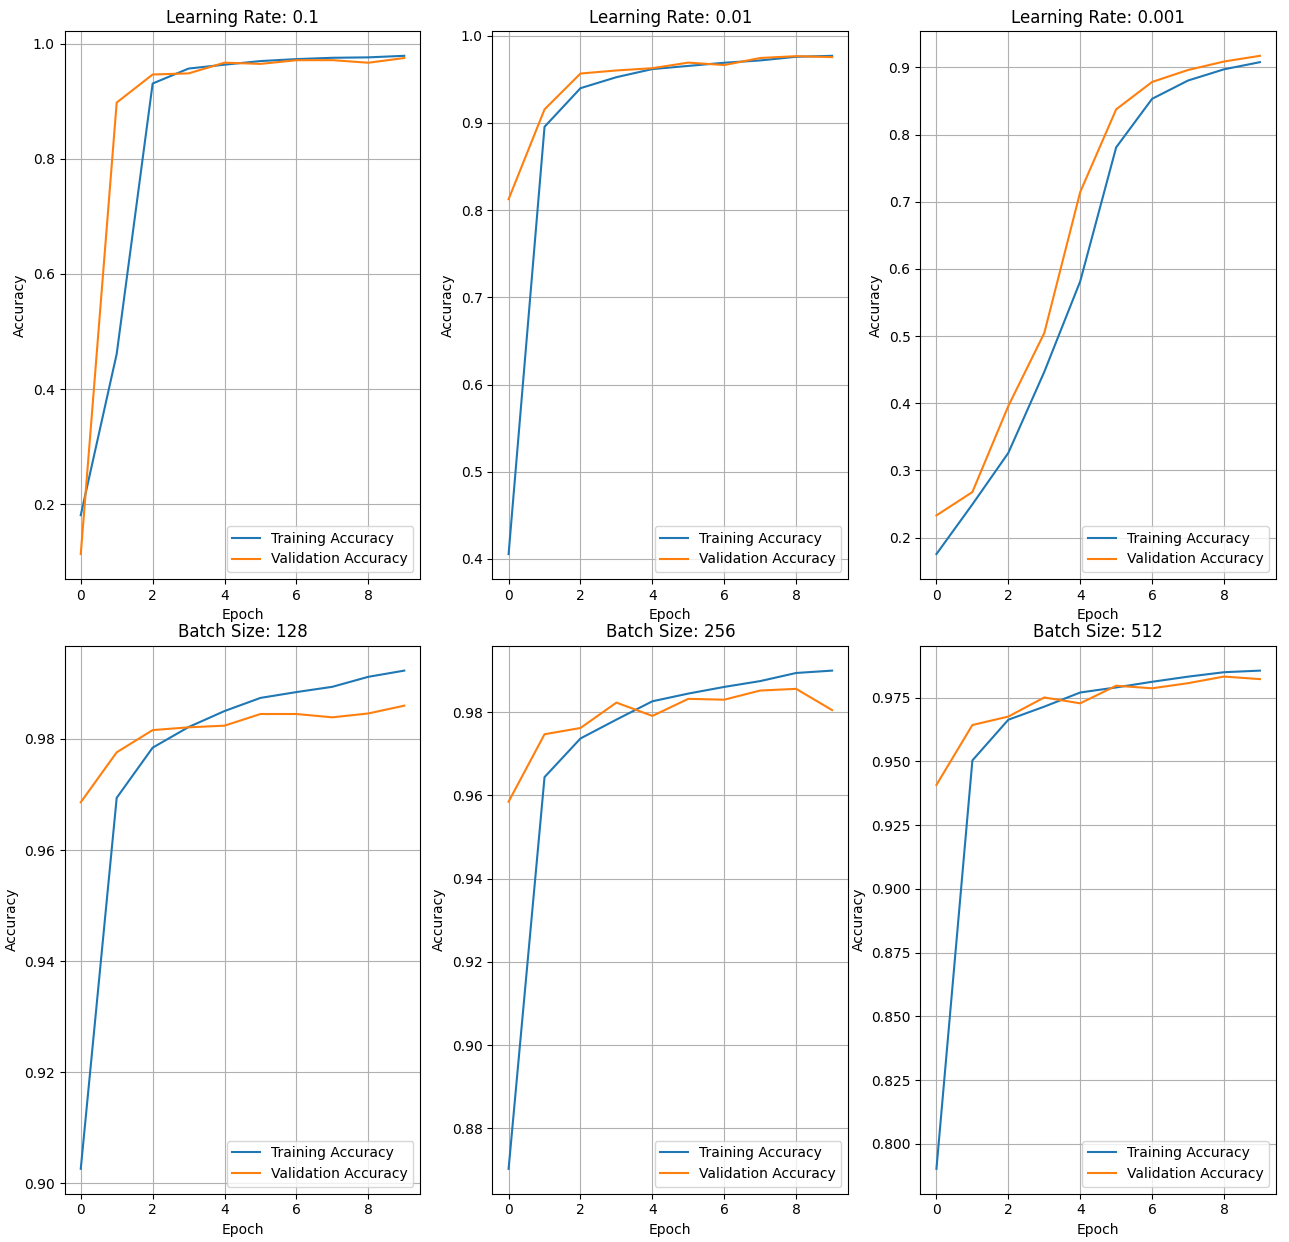
\includegraphics[scale=0.4]{images/learning-rate-batch-size-cnn.png}
    \caption{Performance of training the CNN model with varying learning rates and batch sizes.}
    \label{fig:training-params}
\end{figure}

The learning rate parameter influences how drastically the model weights will change on each weight update. As a result, a smaller learning rate causes model convergence to take longer, as is evident in Figure~\ref{fig:training-params} where the learning rate is set to 0.001. However, this can be a good thing as it allows for more stable results and reduces over-fitting as it gives the model more chances to explore the feature space. The results for the model with the smallest learning rate in Figure~\ref{fig:training-params} show this with the validation accuracy being greater than the training accuracy, at the cost of a smaller validation accuracy compared to the other models. The batch size parameter affects the number of training examples used per gradient update when training the model. Hence, mini-batch gradient descent is being used. The batch size will directly influence the speed of model training, as well as the performance of the trained model. A larger batch size will result in the gradient being calculated fewer times, potentially providing a speedup to the training process. In addition to this, a larger batch size can reduce over-fitting as the noise introduced into the gradient from outliers in the training data is averaged over a larger number of samples, as demonstrated in Figure~\ref{fig:training-params} for the model trained with a batch size of 512.

\newpage
\section{Conclusion}

\newpage
% Bibliography/Reference Stuff
\nocite{*}
\bibliographystyle{abbrv}
\bibliography{main}

\renewcommand{\thesection}{Appendix \Alph{section}: \hspace{-4mm}}
\setcounter{section}{0} % Reset section counter

\newpage
\section{Adaboost with ID3 Base Learner Code}
\label{section:adaboost-code}
\textbf{tree.py}
\begin{lstlisting}[basicstyle= \scriptsize]
class BinaryDecisionTree:
    """ BinaryDecisionTree represents a binary tree
    implementation used for the ID3 decision tree
    training algorithm. Each tree contains 4 parameters:
        - Feature Index:    The current feature index the tree splits on
        - Value:            The value of Feature the determins the split
        - True Branch:      The branch when Feature > Value
        - False Branch:     The branch when Feature <= Value
    """
    def __init__(self, feature_idx, value):
        self.feature_idx = feature_idx
        self.value = value
        self.true_branch = None
        self.false_branch = None

    def add_true(self, branch):
        self.true_branch = branch

    def add_false(self, branch):
        self.false_branch = branch

    def traverse(self, data_row):
        if (self.true_branch is None and self.false_branch is None):
            return self.value

        feature_value = data_row[self.feature_idx]
        if (feature_value > self.value):
            return self.true_branch.traverse(data_row)
        else:
            return self.false_branch.traverse(data_row)

    def print_tree(self, features, level=0):
        if (self.false_branch is not None):
            self.false_branch.print_tree(level + 1)
        print(' ' * 4 * level + '->' + f"{features.columns[self.feature_idx]}: {self.value}")
        if (self.true_branch is not None):
            self.true_branch.print_tree(level + 1)
\end{lstlisting}

\textbf{id3.py}
\begin{lstlisting}[basicstyle= \scriptsize]
import numpy as np                      # For data calculation
from itertools import starmap           # For quickly iterating over features
from tree import BinaryDecisionTree     # Tree implementation

class ID3Classifier:
  """ An implmentation of the Iterative Dichotomiser 3
  (ID3) decision tree algorithm. Constructor parameters
  include an optional depth paramter that controls the maximum
  depth of generated decision trees (default = +infinity).
  This ID3 implementation uses a weighted information gain calculation
  to determine the best feature to split on, and the best value
  of that feature to split on. The decision trees produced are 
  binary decision trees, where each node posesses a split feature
  and split feature value, and the two child branches are 
  designated for examples with feature values less than or
  equal to the split feature value (false branch), and
  values greater than the split feature value (true branch).
  This tree implementation is found in tree.py.
  """
  def __init__(self, depth=np.inf):
    self.depth = depth
    self.tree = None

  def train(self, examples, features, targets):
    """ Public method for training a decision tree using the 
    ID3 algorithm implemented in _train. This public facing
    method sets the tree member of the ID3Classifier class.
    """
    self.tree = None
    self.tree = self._train(examples, features, targets, 1) 

  def _train(self, examples, features, targets, depth):
    """ Implementation of the ID3 decision tree
    induction algorithm used for classification.
    This is a recursive algorithm that choses the next
    feature to evaluate based on each feature's descriminatory
    power, or which feature will result in the most information
    gain about the data. This will continue until 1 of the 3
    following base cases is met:
      1.  Every training instance remaining has the same
          target feature value. In this case, return the
          target feature value. This enables ID3 to return
          the shortest (shallowest) possible trees.

      2.  There are no descriptive features remaining
          to divide the data based on. In this case, select
          the target feature value of majority in the data.

      3.  There are no training instances remaining in the
          data set. In this case, take the target feature value
          of majority in the parent (caller). This demonstrates
          the generalization power of ID3.
    """
    target_counts = targets.value_counts()
    majority_target = target_counts.index.to_numpy()[0][0]

    # Note, the third
    # base case explained above is handled in the recursive
    # call section as we check for an empty new feature list
    # before we even issue the recursive call. Also adding a check
    # here for if we've reached our max tree depth.
    if (len(features) == 0 or target_counts.size == 1 or depth >= self.depth):
      # Return the target value of majority in current data set if
      # there are no features left to partition by, or return
      # the only remaining target value if there is only 1 remaining.
      return BinaryDecisionTree(0, majority_target)

    # Determine the optimal feature and feature value to partition
    # the dataset into true and false branches
    split_feature, split_value = ID3Classifier._calc_split_attribute(examples, features, targets) 
    # Determine the index of the split feature from the columns
    # of the entire dataset, i.e., all features
    split_feature_idx = examples.columns.get_loc(split_feature)

    # Remove the chosen best feature from the list of feature names
    pruned_features = np.delete(features, np.where(features == split_feature))

    # Create a new DecisionTree to be returned
    dt = BinaryDecisionTree(split_feature_idx, split_value)

    # Create the true and false branches based on split feature
    false_branch = examples[examples[split_feature] <= split_value]
    true_branch = examples[examples[split_feature] > split_value]

    # Spawn recursive calls for true and false branches of decision tree, checking
    # for base case first where there are no features left in these trees so we just
    # return the current target value of majority as a leaf
    if (false_branch.empty):
      dt.add_false(BinaryDecisionTree(0, majority_target))
    else:
      dt.add_false(self._train(false_branch, pruned_features, targets.loc[false_branch.index], depth + 1))

    if (true_branch.empty):
      dt.add_true(BinaryDecisionTree(0, majority_target))
    else:
      dt.add_true(self._train(true_branch, pruned_features, targets.loc[true_branch.index], depth + 1))

    return dt


  def predict(self, examples):
    """ Predict the target values given testing examples
    and a tree that has already been trained by the train method.
    """
    if (self.tree is None):
      print("Must train model using train() method first.")
      return []

    predictions = [None for _ in range(examples.shape[0])]
    for i, row in enumerate(examples.to_numpy()):
      predictions[i] = self.tree.traverse(row) 

    return predictions
  
  @staticmethod
  def _calc_entropy(targets):
    """ Calculate the entropy for a sample
    of training examples based on Shanon's 
    Entropy Model. The first column in the passed
    targets Dataframe is taken as the target
    to calculate the entropy against.
    """
    target_name = targets.columns.values[0]
    entropy = 0
    n_targets = targets.shape[0]
    for frequency in targets[target_name].value_counts():
      probability = frequency / n_targets 
      entropy -= probability * np.log2(probability)

    return entropy

  @staticmethod
  def _calc_attribute_info_gain(examples, n_samples, targets, total_entropy, feature):
    # Iterate through each unique value of this feature
    # and calculate the information gain of having this unique
    # value be the split value for this feature 
    unique_values = examples[feature].unique()

    # Calculate the less than or equal to and the greater than
    # splits of the data set using the unique values for this feature.
    # This creates an array of Dataframes of length len(unique_values)
    less_subsets = [examples.loc[examples[feature] <= value] for value in unique_values] 
    greater_subsets = [examples.loc[examples[feature] > value] for value in unique_values]

    # Calculate the entropy for each of the less than or equal to, and greater than, subsets 
    # of the data set for all unique values of this feature.
    less_entropy = np.array([(subset["weight"].to_numpy().sum() / n_samples) * ID3Classifier._calc_entropy(targets.loc[subset.index]) for subset in less_subsets])
    greater_entropy = np.array([(subset["weight"].to_numpy().sum() / n_samples) * ID3Classifier._calc_entropy(targets.loc[subset.index]) for subset in greater_subsets])

    split_info_gain = np.add(less_entropy, greater_entropy)

    info_gains = [total_entropy - split_gains for split_gains in split_info_gain]

    # Find the maximum info gain and its index
    max_info_gain_idx = np.argmax(info_gains)
    max_info_gain = info_gains[max_info_gain_idx]

    return max_info_gain, unique_values[max_info_gain_idx], feature

  @staticmethod
  def _calc_split_attribute(S, feature_names, targets):
    """ Given the dataset S, determine which attribute
    of the dataset and value of that attribute is optimal 
    to partition the data set. The attribute and split value
    is calculated based on the information gain of splitting
    each unique value for a given attribute and taking the 
    largest gain.
    """
    # The number of entries in dataset S
    S_size = S.shape[0]

    # Calculate the entropy for the entire dataset
    e = ID3Classifier._calc_entropy(targets)

    # Build the argument list, which is a list of tuples
    # where each tuple holds the 5 arguments to the function
    n_features = len(feature_names)
    arg_list = zip([S for _ in range(n_features)],
                   [S_size for _ in range(n_features)],
                   [targets for _ in range(n_features)],
                   [e for _ in range(n_features)],
                   feature_names)
    
    # Execute the multi-processing *map operation
    attribute_split_info_gains = starmap(ID3Classifier._calc_attribute_info_gain, arg_list)

    # Pull out the optimal split value and feature based on the maximum info gain
    _, split_value, split_feature = max(list(attribute_split_info_gains), key=lambda item: item[0])

    return split_feature, split_value
\end{lstlisting}

\textbf{adaboost.py}
\begin{lstlisting}[basicstyle= \scriptsize]
import numpy as np                      # Access to math operators
from id3 import ID3Classifier           # ID3 Algorithm implementation

class AdaBoost:
  """ An implementation of the Adaptive Boost
  (Adaboost) boosting classifier that uses
  a custom implementation of the ID3 Decision Tree
  algorithm as a weak base learner. Constructor 
  parameters include T, the number of estimators
  to use when training, and the optional depth parameter,
  which controls the maximum depth of each decision
  tree (default = +infinity).
  """
  def __init__(self, T, depth=np.inf):
    self.T = T
    self.depth = depth
    self.models = [None for _ in range(T)]
    self.alphas = [0.0 for _ in range(T)]

  def train(self, examples, targets):
    """ Use the AdaBoost ensemble learning method
    with ID3 as a base learner to learn a strong 
    hypothesis for the provided data set X_train.
    """
    # How many training examples we are training on
    n_examples = examples.shape[0]

    # Extract the name of the target value we 
    # are trying to classify in y_train
    target_name = targets.columns.values[0]

    # Before we add the weight column, extract the 
    # names of each feature in X_train
    features = examples.columns.values

    # Assign an initial weight to all training examples
    examples["weight"] = [1/n_examples] * n_examples

    # We now have to train T different decision trees 
    # using the provided data. After each tree is trained,
    # we must determine the total error of that decision 
    # tree (sum of weights of incorrectly classified examples)
    # and use the total error to assign a weight to
    # the decision tree.
    self.models = [ID3Classifier(self.depth) for _ in range(self.T)]
    for t in range(self.T):
      # Obtain a weak hypothesis using the ID3 base learner implementation
      self.models[t].train(examples, features, targets)

      # Create an array of prediction results where 1 represents a correct
      # prediction and -1 represents an incorrect prediction
      prediction_booleans = self.models[t].predict(examples) == targets[target_name]
      prediction_results = [1 if pred else -1 for pred in prediction_booleans.values]

      # Calculate the error from the incorrect predictions
      dt_error = examples.loc[prediction_booleans[prediction_booleans == False].index]["weight"].to_numpy().sum()

      # Determine the weight of this tree based on the total error of the tree    
      if (dt_error == 0):
        self.alphas[t] = 1
      #elif (dt_error >= 0.5):
      #  break
      else:
        EPS = 1e-10 # Account for divide by zero
        self.alphas[t] = 0.5 * np.log((1 - dt_error) / (dt_error + EPS)) 

      # Update example weights based on if they were correctly
      # or incorrectly classified with following formulas:
      #   (correctly classified): example weight * e^(-tree weight) 
      #   (incorrectly classified): example weight * e^(tree weight)
      # we levereage the prediction_results array here since it contains
      # 1 for each correct classification and -1 for each incorrect classification
      examples["weight"] *= np.exp(-self.alphas[t] * np.array(prediction_results))

      # Normalize the new sample weights so they add to 1
      examples["weight"] /= examples["weight"].to_numpy().sum()

  def predict(self, examples):
    """ Use list of weak hypothesis and alphas trained
    with the train method to build a strong hypothesis 
    for each training example providede. The classification
    of each provided training example is returned in an array.
    """
    n_examples = examples.shape[0]

    # Populate a 2D array of all predictions made by each model for each example
    predictions = np.array([[None for _ in range(n_examples)] for _ in range(self.T)])
    for t in range(self.T):
      predictions[t] = self.models[t].predict(examples)

    # If only 1 tree was trained, just return the predictions
    if (self.T == 1):
      return predictions[0]

    # Iterate through each prediction and compare them to
    # predictions made by other trees based off weight
    # to determine the 'true' prediction
    true_predictions = ['' for _ in range(n_examples)]
    for i in range(n_examples):
      example_predictions = predictions[:, i]
      prediction_weights = {} 
      for j, pred in enumerate(example_predictions):
        if pred in prediction_weights:
          prediction_weights[pred] += self.alphas[j]
        else:
          prediction_weights[pred] = self.alphas[j]

      top_prediction = example_predictions[0] 
      top_weight = -1
      for pred, weight in prediction_weights.items():
        if weight >= top_weight:
          top_weight, top_prediction = weight, pred

      true_predictions[i] = top_prediction

    return true_predictions
\end{lstlisting}

\textbf{main.py}
\begin{lstlisting}[basicstyle= \scriptsize]
import pandas as pd               # For data manipulation and analysis
import time                       # For execution timing
import random                     # Random number generation

import matplotlib.pyplot as plt                               # For visualization
import seaborn as sns                                         # Advanced visualizations
from sklearn.metrics import accuracy_score, confusion_matrix  # For model evaluation
from sklearn.model_selection import train_test_split          # For splitting the data
from ucimlrepo import fetch_ucirepo                           # Letter recognition data set

from adaboost import AdaBoost

def estimator_benchmark(features, targets, T=50):
  """ Benchmark the Adaboost implementation
  found in Adaboost.py by running training/testing
  sessions on the provided features and targets but
  varying the number of estimators, or weak hypotheses
  learned by the Adaboost algorithm during each session.
  Returns a Dataframe containing the following:
    - Test data 'random state' integer (for reproducibility).
    - Accuracy of training.
    - Depth of learned tree.
    - Number of estimators
    - Time taken training model.
    - Time taken classifying.
  """
  # Fetch the dataset and sort into features/targets.
  letter_recognition = fetch_ucirepo(id=59) 
  features = letter_recognition.data.features
  targets = letter_recognition.data.targets
  
  # Depth of learned binary decision tree for each test
  depth = len(features.columns) 

  # Number of estimators to test during each session
  estimator_tests = range(1, T)
  n_estimator_tests = len(estimator_tests)

  # Choose a random state to split the data on
  state = random.randint(1, 2**30)

  # Map of returned data.
  results = {'State': [state for _ in range(n_estimator_tests)],
             'Accuracy': [0.0 for _ in range(n_estimator_tests)],
             'Depth': [depth for _ in range(n_estimator_tests)],
             'Estimators': estimator_tests,
             'Train Time': [0.0 for _ in range(n_estimator_tests)],
             'Classify Time': [0.0 for _ in range(n_estimator_tests)]
             }
  
  # Split using a random state.
  X_train, X_test, y_train, y_test = train_test_split(features, targets, test_size=0.2, random_state=state)

  # Perform n tests.
  for n in range(n_estimator_tests):
    # Number of estimators to use for current test
    estimators = estimator_tests[n]

    # Copy the dataframes into this iteration's datasets
    training_examples = X_train.copy(deep=True)
    training_targets = y_train.copy(deep=True)

    # Test the AdaBoost algorithm for 1 to 100 estimators.
    ada = AdaBoost(estimators, depth) 

    # Train the AdaBoost classifier and time how long it takes.
    start_train_time = time.time()
    ada.train(training_examples, training_targets)
    results['Train Time'][n] = time.time() - start_train_time 

    # Predict testing data
    start_classify_time = time.time()
    y_pred = ada.predict(X_test)
    results['Classify Time'][n] = time.time() - start_classify_time

    results['Accuracy'][n] = accuracy_score(y_test, y_pred)

  return pd.DataFrame(results)



def depth_benchmark(features, targets):
  """ Benchmark the Adaboost implementation
  found in Adaboost.py by running training/testing
  sessions on the provided features and targets but
  varying the depth of the learned trees on each session.
  Returns a Dataframe containing the following:
    - Test data 'random state' integer (for reproducibility).
    - Accuracy of training.
    - Depth of learned tree.
    - Number of estimators
    - Time taken training model.
    - Time taken classifying.
  """
  # Fetch the dataset and sort into features/targets.
  letter_recognition = fetch_ucirepo(id=59) 
  features = letter_recognition.data.features
  targets = letter_recognition.data.targets

  # Test from depth 1 to the number of features + 5
  depths = range(1, len(features.columns) + 5)
  n_depths = len(depths)

  # Choose a randome state to split the data on
  state = random.randint(1, 2**30)

  # The number of estimators for training
  t = 1 

  # Map of returned data.
  results = {'State': [state for _ in range(n_depths)],
             'Accuracy': [0.0 for _ in range(n_depths)],
             'Depth': depths,
             'Estimators': [t for _ in range(n_depths)],
             'Train Time': [0.0 for _ in range(n_depths)],
             'Classify Time': [0.0 for _ in range(n_depths)]
             }
  
  # Split using a random state.
  X_train, X_test, y_train, y_test = train_test_split(features, targets, test_size=0.2, random_state=state)

  # Perform n tests.
  for n in range(n_depths):
    # Depth of learned decision tree for current test
    depth = depths[n]

    # Copy the dataframes into this iteration's datasets
    training_examples = X_train.copy(deep=True)
    training_targets = y_train.copy(deep=True)

    # Test the AdaBoost algorithm for 1 to 100 estimators.
    ada = AdaBoost(t, depth) 

    # Train the AdaBoost classifier and time how long it takes.
    start_train_time = time.time()
    ada.train(training_examples, training_targets)
    results['Train Time'][n] = time.time() - start_train_time 

    # Predict testing data
    start_classify_time = time.time()
    y_pred = ada.predict(X_test)
    results['Classify Time'][n] = time.time() - start_classify_time

    results['Accuracy'][n] = accuracy_score(y_test, y_pred)

  return pd.DataFrame(results)


def adaboost_benchmark(features, targets, N=10, display_confusion_matrix=False):
  """ Benchmark the Adaboost implementation
  found in Adaboost.py by running N training/testing
  sessions on the provided features and targets. 
  Returns a Dataframe containing the following:
    - Test data 'random_state' integer (for reproducibility).
    - Accuracy of training.
    - Depth of learned tree.
    - Number of estimators
    - Time taken training model.
    - Time taken classifying.
  """
  # Fetch the dataset and sort into features/targets.
  letter_recognition = fetch_ucirepo(id=59) 
  features = letter_recognition.data.features
  targets = letter_recognition.data.targets

  # Depth of learned binary decision tree for each test
  depth = len(features.columns) 

  # Number of estimators 
  t = 14 

  # Map of returned data.
  results = {'State': random.sample(range(1, 2**30), N),
             'Accuracy': [0.0 for _ in range(N)],
             'Depth': [depth for _ in range(N)],
             'Estimators': [t for _ in range(N)],
             'Train Time': [0.0 for _ in range(N)],
             'Classify Time': [0.0 for _ in range(N)]
             }
  
  # Perform n tests.
  for n in range(N):
    # Split using a random state.
    X_train, X_test, y_train, y_test = train_test_split(features, targets, test_size=0.2, random_state=results['State'][n])

    # Copy the dataframes into this iteration's datasets
    training_examples = X_train.copy(deep=True)
    training_targets = y_train.copy(deep=True)

    # Test the AdaBoost algorithm for 1 to 100 estimators.
    ada = AdaBoost(t, depth) 

    # Train the AdaBoost classifier and time how long it takes.
    start_train_time = time.time()
    ada.train(training_examples, training_targets)
    results['Train Time'][n] = time.time() - start_train_time 

    # Predict testing data
    start_classify_time = time.time()
    y_pred = ada.predict(X_test)
    results['Classify Time'][n] = time.time() - start_classify_time

    results['Accuracy'][n] = accuracy_score(y_test, y_pred) * 100.00

    if (display_confusion_matrix):
      labels = targets["lettr"].unique()
      conf_matrix = confusion_matrix(y_test, y_pred, labels=labels)
      df_cm = pd.DataFrame(conf_matrix, index=labels, columns=labels)
      plt.figure(figsize=(6, 4))
      sns.heatmap(df_cm, annot=True, cmap='Blues', fmt='d', cbar=False)
      plt.title("Confusion Matrix Heatmap")
      plt.xlabel("Predicted Labels")
      plt.ylabel("True Labels")
      plt.show()

  return pd.DataFrame(results)


if __name__ == '__main__':
  # fetch dataset 
  letter_recognition = fetch_ucirepo(id=59) 

  # Store the features and targets
  features = letter_recognition.data.features
  targets = letter_recognition.data.targets

  # Store a combination of features and targets
  total = pd.DataFrame(data=letter_recognition.data.original, columns=letter_recognition.data.headers)

  # Check for any missing values
  print(total.isnull().sum())

  # Get summary statistics of the data
  print(total.describe())

  # Check the distribution of target labels
  for label in targets.columns.values:
    print(total[label].value_counts())

  benchmark_results = adaboost_benchmark(features, targets, N=1, display_confusion_matrix=True)
  # benchmark_results = depth_benchmark(features, targets)
  # benchmark_results = estimator_benchmark(features, targets, 20)
  print(benchmark_results)

  # Save to csv
  benchmark_results.to_csv('benchmark.csv', index=False)
\end{lstlisting}

\newpage
\section{Neural Network Code}
\textbf{Importing Packages:}
\begin{lstlisting}[basicstyle= \scriptsize]
# import packages:
from ucimlrepo import fetch_ucirepo                   # used to fetch dataset
import numpy as np                                    # used for math operations
import pandas as pd                                   # used to manipulate data
from sklearn.model_selection import train_test_split  # used to split the data
from sklearn.metrics import confusion_matrix          # used to make cm
from sklearn.preprocessing import StandardScaler      # used to standardize the data
import csv                                            # used to load CSVs

import seaborn as sns                 # used for visualization of confusion matrix
import matplotlib.pyplot as plt       # used for visualization of training loss
\end{lstlisting} 

\textbf{Loading the Dataset:}
\begin{lstlisting}[basicstyle= \scriptsize]
# because the dataset is from the UCI ML repo, we can use their functions to fetch from their website:
breast_data = fetch_ucirepo(id = 17)

# can now access the data:
breast_x = breast_data.data.features    # extract the features from the dict into a pandas data frame
breast_y = breast_data.data.targets     # extract the labels from the dict into a pandas data frame
\end{lstlisting}

\textbf{Examining Dataset Properties:}
\begin{lstlisting}[basicstyle= \scriptsize]
# get the total number of instances:
print(f"there are {breast_x.shape[0]} examples in the dataset")

# get number of features:
print(f"there are {breast_x.shape[1]} distinct features to train on")

# get the number of unique target variables:
print(f"the available diagnoses are: {breast_y['Diagnosis'].unique()}")

# get the names of the features:
print(f"the available features are: \n")
for col in breast_x.columns:    # for every column in the data frame, 
    print(col)                  # print the column    
\end{lstlisting}

\textbf{Dataset Pre-Processing:}
\begin{lstlisting}[basicstyle= \scriptsize]
# check for null values in the features:
null = breast_x.isnull().values.any()   

# if any null values exist, drop them, else pass
if null == True:
    breast_x = breast_x.dropna() 
    print(f'null values removed from features')
else:
    print(f'no null values detected in features')

# check for null values in the labels, same process as above
null = breast_y.isnull().values.any()
if null == True:
    breast_y = breast_y.dropna()
    print(f'null values removed from labels')
else:
    print(f'no null values detected in labels')
    
# standardize values by defining a scaler and fitting data to scaler:
scaler = StandardScaler()
x_scaled = pd.DataFrame(scaler.fit_transform(breast_x))
print('features scaled')

# encode benign to 0, and malignant to 1
breast_y =  pd.DataFrame(breast_y['Diagnosis'].map(lambda row: 1 if row == 'M' else 0))
print('labels encoded: M = 1, B = 0')
breast_y.head()

# partition data -> want 70% train, 15% validation, 15% testing
x_train, dummy_x, y_train, dummy_y = train_test_split(x_scaled, breast_y, train_size = 0.7, test_size = 0.3)
x_val, x_test, y_val, y_test = train_test_split(dummy_x, dummy_y, train_size = 0.5, test_size = 0.5)

print(f"training data has form: {x_train.shape}, labels are: {y_train.shape}")
print(f"validation data has form: {x_val.shape}, labels are: {y_val.shape}")
print(f"test data has form: {x_test.shape}, labels are: {y_test.shape}")
\end{lstlisting}

\newpage
\textbf{Function Definition:}
\begin{lstlisting}[basicstyle= \scriptsize]
# define useful functions:

# logistic sigmoid function
def sigmoid(x):
    return 1 / (1 + np.exp(-x))

# derivative of the sigmoid function
def sigmoid_derivative(x):
    return sigmoid(x) * (1 - sigmoid(x))

# rectified linear unit (basically a straight line)
def relu(x):
    return np.maximum(0, x)

# derivative function of relu (accepts np.arrays)
def relu_derivative(x):
    return (x > 0).astype(float)

# binary cross entropy -> for binary classification between 0 & 1
def binary_crossentropy_loss(target, output):
    output = np.clip(output, 1e-10, 1 - 1e-10)                              # clip to prevent log 0
    loss = - (target * np.log(output) + (1 - target) * np.log(1 - output))  # BCE formula
    return loss    
\end{lstlisting}

\textbf{Neural Network Class Definition:}

\begin{lstlisting}[basicstyle= \scriptsize]
# create neural network class:
"""
this class accepts:

input_size: number of input neurons
hidden_size: number of hidden neurons
output_size: expected number of output neurons
load: whether or not to load initialized weights

"""
class NeuralNetwork:
    # constructor:
    def __init__(self, input_size, hidden_size, output_size, load):
        # assign function inputs as instance variables:
        self.input_size = input_size        # assign input neurons
        self.hidden_size = hidden_size      # assign hidden neurons
        self.output_size = output_size      # assign output neurons

        # if the user wants to load the pre-initialized weights and biases:
        if load == True:
            # open the CSV and read it:
            with open('initial_weights.csv', 'r') as f:
                reader = csv.reader(f)

                # for every value in each row, return as float to np.array:
                w1_flat = np.array([float(val) for val in next(reader)])
                b1_flat = np.array([float(val) for val in next(reader)])
                w2_flat = np.array([float(val) for val in next(reader)])
                b2_flat = np.array([float(val) for val in next(reader)])

                # ensure that weights are in the correct dimensions:
                self.w1 = w1_flat.reshape(hidden_size, input_size)
                self.b1 = b1_flat.reshape(hidden_size, 1)
                self.w2 = w2_flat.reshape(output_size, hidden_size)
                self.b2 = b2_flat.reshape(output_size, 1)

                # print to user that it was a success:
                print('weights loaded')
                print("w1 shape:", self.w1.shape, 'w1 type:', type(self.w1))
                print("b1 shape:", self.b1.shape, 'b1 type:', type(self.b1))
                print("w2 shape:", self.w2.shape, 'w2 type:', type(self.w2))
                print("b2 shape:", self.b2.shape, 'b2 type:', type(self.b2))

        # if not, randomly initialize weights and biases for the layers:
        else:

            # from input to hidden:
            self.w1 = np.random.randn(hidden_size, input_size)
            self.b1 = np.random.randn(hidden_size, 1)

            # from hidden to output:
            self.w2 = np.random.randn(output_size, hidden_size)
            self.b2 = np.random.randn(output_size, 1)

            # print to user that it was a success:
            print('weights randomly initialized')
            print("w1 shape:", self.w1.shape, 'w1 type:', type(self.w1))
            print("b1 shape:", self.b1.shape, 'b1 type:', type(self.b1))
            print("w2 shape:", self.w2.shape, 'w2 type:', type(self.w2))
            print("b2 shape:", self.b2.shape, 'b2 type:', type(self.b2))


    # feedforward function:
    def forward_pass(self, x):
        # make sure x is a column vector:
        x = x.reshape((self.input_size, 1))

        # from input to hidden:
        self.net1 = np.dot(self.w1, x) + self.b1    # calculate net1
        self.h1 = relu(self.net1)                   # calculate output of hidden layer

        # from hidden to output:
        self.net2 = np.dot(self.w2, self.h1) + self.b2  # calculate net2
        self.o = sigmoid(self.net2)                     # calculate output of network

        return self.o       # return value to user
    
    # backpropagation:
    def backward_pass(self, x, y, learning_rate):
        # make sure x is a column vector:
        x = x.reshape((self.input_size, 1))

        # get o - t:
        o_error = self.o - y

        # get gradients for weights and biases at the output layer:
        de_dw2 = np.dot((o_error * sigmoid_derivative(self.net2)), self.h1.T)   # this is the partial derivative of E wrt. W2
        de_db2 = o_error * sigmoid_derivative(self.net2)                        # this is the partial derivative of E wrt. B2

        # get gradients for weights and biases at the input layer:

        # this is an intermediary value because I was getting lost in the matrix dimensions
        delta_1 = np.dot(self.w2.T, o_error * sigmoid_derivative(self.net2)) * relu_derivative(self.net1)  
        de_dw1 = np.dot(delta_1, x.T)   # this is the partial derivative of E wrt. W1
        de_db1 = delta_1                # this is the partial derivative of E wrt. B1

        # update weights and biases:
        self.w1 -= learning_rate  * de_dw1  # update w1
        self.b1 -= learning_rate  * de_db1  # update b1
        self.w2 -= learning_rate  * de_dw2  # update w2
        self.b2 -= learning_rate  * de_db2  # update b2

    # training:
    def train(self, x_train, y_train, x_val, y_val, epochs, learning_rate):
        # used in the plotting:
        self.epochs = epochs
        
        # initialize lists for appending train and val history to:
        train_loss_history = []
        val_loss_history = []

        # for every epoch:
        for epoch in range(epochs):
            total_train_loss = 0    # reset train loss for new epoch
            total_val_loss = 0      # reset val loss for new epoch

            # training loop:
            for i in range(x_train.shape[0]):
                # extract example:
                x = x_train.iloc[i].values

                # get target for that example:
                target = y_train.iloc[i].values

                # compute forward pass:
                output = self.forward_pass(x)

                # backpropagate:
                self.backward_pass(x, target, learning_rate)

                # get loss:
                loss = binary_crossentropy_loss(target, output)
                total_train_loss += loss    # add to total loss  

            # get average BCE for train for that epoch:
            average_train_loss_per_epoch = total_train_loss / x_train.shape[0]
            train_loss_history.append(average_train_loss_per_epoch)

            # validation loop:
            for i in range(x_val.shape[0]):
                # extract example:
                x = x_val.iloc[i].values

                # get target for that example:
                target = y_val.iloc[i].values

                # compute forward pass:
                output = self.forward_pass(x)

                # get loss:
                loss = binary_crossentropy_loss(target, output)
                total_val_loss += loss    # add to total loss 
            
            # get average BCE for val:
            average_val_loss_per_epoch = total_val_loss / x_val.shape[0]
            val_loss_history.append(average_val_loss_per_epoch)

            # print values to user:
            print(f"epoch: {epoch + 1}/{epochs} 
                    | train loss was: {round(float(average_train_loss_per_epoch), 6)} 
                    | val loss was: {round(float(average_val_loss_per_epoch), 6)}")  

        return np.array(train_loss_history).reshape(-1, 1), np.array(val_loss_history).reshape(-1, 1)

    # testing:
    def test(self, x_test, y_test):
        # need to get the output for each value of x_test, compare against y_test:
        correct_predictions = 0

        # initialize lists for appending values to:
        targets = []
        predictions = []

        for i in range(x_test.shape[0]):
            # extract example:
            x = x_test.iloc[i].values

            # extract target:
            target = y_test.iloc[i].values

            # compute forward pass:
            output = self.forward_pass(x)

            # get class value from sigmoid value if over threshold:
            prediction = 1 if output >= 0.5 else 0

            print(f"predicted: {prediction} | true: {target}")

            # append to lists, these are used for confusion matrix:
            predictions.append(prediction)
            targets.append(target)

            # if correct, add to successes:
            if prediction == target:
                correct_predictions += 1

        # print accuracy:
        accuracy = round((correct_predictions / x_test.shape[0]) * 100, 3)
        print(f"accuracy of model is: {accuracy}")

        return predictions, targets, accuracy   
\end{lstlisting}

\textbf{Training the Model:}

\begin{lstlisting}[basicstyle= \scriptsize]
# instantiate a network:
nn = NeuralNetwork(input_size = 30, hidden_size = 15, output_size = 1, load = True)

# run the training with the hyperparameters you want, return losses for plotting:
train_loss_history, val_loss_history = nn.train(x_train, y_train, x_val, y_val, epochs = 1000, learning_rate = 0.001)

# plotting stuff:
epochs = np.arange(1, nn.epochs + 1, 1).reshape(-1,1)

# plot training & validation loss:
fig = plt.figure(figsize = (12,6))
plt.plot(epochs, train_loss_history, label = 'training')
plt.plot(epochs, val_loss_history, label = 'validation')
plt.title('loss vs. epochs')
plt.ylabel('average binary crossentropy loss per sample')
plt.xlabel('epochs')
plt.legend()
plt.xlim([1, nn.epochs])
plt.grid('both')
plt.show()
\end{lstlisting}

\newpage
\textbf{Testing the Model:}
\begin{lstlisting}[basicstyle= \scriptsize]
# take the model that is already trained and use it to predict the class of tumour based on data:
predictions, targets, accuracy = nn.test(x_test, y_test)

# generate a confusion matrix:
cm = confusion_matrix(targets, predictions)

# plot the confusion matrix:
sns.heatmap(cm, annot=True, fmt='d', cmap='Blues', xticklabels=['Benign', 'Malignant'], yticklabels=['Benign', 'Malignant'])
plt.xlabel('Predicted')
plt.ylabel('True')
plt.title('Confusion Matrix')
plt.show()
\end{lstlisting}

\newpage
\section{Naive Bayes Code}
\textbf{Library and data import}
\begin{lstlisting}
from ucimlrepo import fetch_ucirepo
import pandas as pd
import numpy as np
from sklearn.model_selection import train_test_split
from collections import defaultdict

# Fetch the dataset
car_dataset = fetch_ucirepo(id=19)

# Data unpacking
X = car_dataset.data.features
y = car_dataset.data.targets

# Train test split
X_train, X_test, y_train, y_test = train_test_split(X,y, test_size = 0.1,random_state=12)

# variable information 
print(car_dataset.variables)
\end{lstlisting}

The following code blocks were for data exploration.

\begin{lstlisting}
print(type(X))
print(type(y))

# Display the statistics in the dataset along the features
print(f"{X.describe()} \n")

# Display some random samples
X.sample(10)
\end{lstlisting}

\begin{lstlisting}
# Concatenate the feature and label data frames
df = pd.concat([X,y],axis=1)
print(df.sample(10))
# Return the class distribution
print("\n===== Number of occurences in each unique class =====")
print(df['class'].value_counts())

df_train = pd.concat([X_train,y_train],axis=1)
print(df_train.shape)
print(df_train['class'].value_counts())

df_test = pd.concat([X_test,y_test],axis=1)
print(df_test.shape)
\end{lstlisting}


\textbf{Functions for determining the prior and conditional probabilities}
\begin{lstlisting}
def find_prior_probs(df, label_column, minority_class = None):
'''
This function finds the prior probability of each class in the dataframe and report them in a dictionary

Parameters:
- df (pd dataframe): DataFrame from which the probability is determined
- label_colum (str): name of the class/label column
- minority_class (dict): a dictionary containing the name of the minority classes (keu) and the upweighting factor corresponding to the class as (value)

Returns:
- class_prior (dict): the dictionary containing class (key) and their corresponding prior probabilities (value)
'''
classes = df[label_column].unique()                 # List of the classes
num_instances = len(df)
class_prior_probs = {}

for class_value in classes:
    class_count = df[df[label_column]==class_value].shape[0]
    
    # if there is a weighting factor defined for the current class in the minority_class then use the value as the factor, else 1 (no scaling)
    upweight_factor = minority_class[class_value] if class_value in minority_class else 1      
    class_prior_probs[str(class_value)] = class_count / num_instances * upweight_factor

return class_prior_probs

def find_cond_probs(df, label_column):
classes = df[label_column].unique()

feature_cond_probs = defaultdict(lambda: defaultdict(lambda: defaultdict(float)))
'''This is a nested dictionary of the following structure
    - Level 1 - Class Values: This level has the class values and the next dictionary level as the key-value pair
        - Level 2 - Feature Names: This level of dictionary has the feature name and the next dictionary level as the key-value pair
            - Level 3 - Feature Values: This level of dictionary has the feature value and the conditional probabilities P(feature == feature value | class == class value) as the key-value pair 
'''

# Considering the conditional probability feature by feature
for feature in df.columns:
    # Skip this step if the feature is the label column of the dataframe
    if feature == label_column:
        pass
    
    # Iterate over each class c of the dataframe to find the conditional probabilities of each feature P(feature = value | class)
    for c in classes: 
        df_subset = df[df[label_column]==c]                         # Subset of the dataframe where class has the value c
        feature_count = df_subset[feature].value_counts()           # Get a series with the number of instances of each feature value in the subset

        # Iterate over all the feature values and calculate the conditional probabilities of each value 
        for value, count in feature_count.items():                  
            feature_cond_probs[c][feature][value] = count / len(df_subset)

return feature_cond_probs
\end{lstlisting}

\textbf{Determine the prior and conditional probability}
\begin{lstlisting}
# Define a dictionary with the weighting factors for the minority classes
minority_class = {
    "acc": 1.5,
    "good": 5,
    "vgood": 5
}

# Find the prior probability with the weighting factor
prior_probs = find_prior_probs(df_train,'class',minority_class=minority_class)

for key, value in prior_probs.items():
    print(f"The prior probability of class = {key} is {value*100:.3f}%")
\end{lstlisting}

\begin{lstlisting}
cond_probs = find_cond_probs(df_train,label_column='class')
cond_probs

count = 1
for key_1, value_1 in cond_probs.items():
    for key_2, value_2 in value_1.items():
        for key_3, value_3 in value_2.items():
                print(f"{count} \t p({key_2}=={key_3}|{key_1}) = {value_3:.3f}")
                count += 1
\end{lstlisting}

The code block below shows the Naive-Bayes classifier function, which takes the prior and conditional probability from the dataset to classify testing data.

\begin{lstlisting}
def naive_bayes_classifier(prior_probs, cond_probs, instances):
'''
This function is used for classifying an instance

Parameters
- prior_probs: the dictionary with the prior class probabilities
- cond_probs: the 3-tier dictionary structure returned by the find_cond_probs() function. This structure represents the conditional probabilities P(features | classes) and has the structure of [class value][feature][feature value]
- instance: a dictionary representing a data point with feature_name-feature_value key-value pairs
'''

# Get the list of classes (from the cond_probs structures)
classes = []
for item in cond_probs.items():
    classes.append(item[0]) 

# List of empty dictionaries to store the probabilities of the instance belong to each class
class_probs = [{}] * len(instances)                                      

for index, instance in enumerate(instances):
    # Iterate over each class to find the prior probability 
    for c in classes:
        class_probs[index][c] = prior_probs[c]                     # p(class==c)

        # Iterate over each feature in the instance to find the accumulative of conditional probabilties
        for feature,value in instance.items():
            class_probs[index][c] *= max(cond_probs[c][feature][value],1e-6)       # In case of zero probability, use a small number
    
    class_probs[index] = max(class_probs[index], key=class_probs[index].get)

return class_probs
\end{lstlisting}

\textbf{Test the Naive Bayes classifier}
\begin{lstlisting}
# Drop the index to later concatenate with the predicted label
test_instances = df_test.reset_index(drop=True)

# Extract the features from the test set and reformat it as a list of instance dictionaries
test_instance_features = test_instances.drop('class',axis =1).to_dict(orient='records')

prediction = naive_bayes_classifier(prior_probs=prior_probs,
                                    cond_probs=cond_probs,
                                    instances=test_instance_features)

prediction_df = pd.DataFrame(prediction, columns=["Predicted_Class"])
prediction_result = pd.concat([test_instances,prediction_df],axis=1)

# Draw some random samples to show the prediction results
test_idx = np.random.randint(0,df_test.shape[0],15)
prediction_result.iloc[test_idx]

\end{lstlisting}

\textbf{Performance Evaluation and Visualization}
\begin{lstlisting}
import matplotlib.pyplot as plt 
from sklearn.metrics import accuracy_score, confusion_matrix, ConfusionMatrixDisplay, classification_report

label_true = prediction_result['class']
label_predicted = prediction_result['Predicted_Class']
accuracy = accuracy_score(label_true,label_predicted)
print(f"Accuracy score: {accuracy*100:.2f}%")

class_labels = ['unacc', 'acc', 'good', 'vgood']
cm = confusion_matrix(label_true,label_predicted ,labels = class_labels)
disp = ConfusionMatrixDisplay(confusion_matrix=cm,display_labels=class_labels)
disp.plot(cmap=plt.cm.Blues)

font_size = 20
for text in disp.ax_.texts:
    text.set_fontsize(font_size)  # Adjust the number's font size here
fig = disp.ax_.get_figure()
fig.set_figwidth(12)
fig.set_figheight(10) 
plt.title("Confusion Matrix - Naive Bayes Classifier")
plt.xticks(rotation=90, ha='right', fontsize=font_size-2)                     # Rotate x labels for better readability
plt.yticks(rotation=0,fontsize = font_size-2)                                  # Keep y labels horizontal
plt.xlabel('Prediction', fontsize = font_size)
plt.ylabel('True Label', fontsize = font_size)

plt.tight_layout()
plt.show()

report = classification_report(label_true, label_predicted, labels = class_labels, target_names= class_labels)
print("\nClassification Report:\n", report)
\end{lstlisting}

\newpage
\section{ANN Code - Using Libraries}
\textbf{GPU Hardware Check}
\begin{lstlisting}
import tensorflow as tf

gpus = tf.config.list_physical_devices('GPU')
if gpus:
    try:
    # Currently, memory growth needs to be the same across GPUs
    for gpu in gpus:
        tf.config.experimental.set_memory_growth(gpu, True)
    logical_gpus = tf.config.list_logical_devices('GPU')
    print(len(gpus), "Physical GPUs,", len(logical_gpus), "Logical GPUs")
    except RuntimeError as e:
    # Memory growth must be set before GPUs have been initialized
    print(e)
\end{lstlisting}

\textbf{Data Import and Discovery}
\begin{lstlisting}
    import numpy as np # linear algebra
import struct
from array import array
from os.path import join
import kagglehub


# Download latest version
dataset_path = kagglehub.dataset_download("hojjatk/mnist-dataset")

print("Path to dataset files:", dataset_path)


# MNIST Data Loader Class

class MnistDataloader(object):
    def __init__(self, training_images_filepath,training_labels_filepath,
                 test_images_filepath, test_labels_filepath):
        self.training_images_filepath = training_images_filepath
        self.training_labels_filepath = training_labels_filepath
        self.test_images_filepath = test_images_filepath
        self.test_labels_filepath = test_labels_filepath
    
    # Function to read the labels and load
    def read_images_labels(self, images_filepath, labels_filepath):        
        labels = []
        with open(labels_filepath, 'rb') as file:
            magic, size = struct.unpack(">II", file.read(8))
            if magic != 2049:
                raise ValueError('Magic number mismatch, expected 2049, got {}'.format(magic))
            labels = array("B", file.read())        
        
        with open(images_filepath, 'rb') as file:
            magic, size, rows, cols = struct.unpack(">IIII", file.read(16))
            if magic != 2051:
                raise ValueError('Magic number mismatch, expected 2051, got {}'.format(magic))
            image_data = array("B", file.read())        
        images = []
        for i in range(size):
            images.append([0] * rows * cols)
        for i in range(size):
            img = np.array(image_data[i * rows * cols:(i + 1) * rows * cols])
            img = img.reshape(28, 28)
            images[i][:] = img            
        
        return np.array(images), np.array(labels)
            
    def load_data(self):
        x_train, y_train = self.read_images_labels(self.training_images_filepath, self.training_labels_filepath)
        x_test, y_test = self.read_images_labels(self.test_images_filepath, self.test_labels_filepath)
        return (x_train, y_train),(x_test, y_test)
        
        
# Data Visualization
%matplotlib inline
import random
import matplotlib.pyplot as plt

# Set file paths based on added MNIST Datasets
base_path = 'data'
training_images_filepath = join(base_path, 'train-images-idx3-ubyte/train-images-idx3-ubyte')
training_labels_filepath = join(base_path, 'train-labels-idx1-ubyte/train-labels-idx1-ubyte')
test_images_filepath = join(base_path, 't10k-images-idx3-ubyte/t10k-images-idx3-ubyte')
test_labels_filepath = join(base_path, 't10k-labels-idx1-ubyte/t10k-labels-idx1-ubyte')

# Helper function to show a list of images with their relating titles
def show_images(images, title_texts):
    cols = 5
    rows = int(len(images)/cols)
    plt.figure(figsize=(cols*4,rows*4))
    
    for index, x in enumerate(zip(images, title_texts)):        
        image = x[0]        
        title_text = x[1]
        plt.subplot(rows, cols, index+1)        
        plt.imshow(image, cmap=plt.cm.gray)
        if (title_text != ''):
            plt.title(title_text, fontsize = 15);        


# Load MINST dataset
mnist_dataloader = MnistDataloader(training_images_filepath, training_labels_filepath, test_images_filepath, test_labels_filepath)
(x_trainval, y_trainval), (x_test, y_test) = mnist_dataloader.load_data()


# Show some random training and test images 
images_2_show = []
titles_2_show = []
for i in range(0, 10):
    r = random.randint(1, 60000)
    images_2_show.append(x_trainval[r])
    titles_2_show.append('training image [' + str(r) + '] = ' + str(y_trainval[r]))    

for i in range(0, 5):
    r = random.randint(1, 10000)
    images_2_show.append(x_test[r])        
    titles_2_show.append('test image [' + str(r) + '] = ' + str(y_test[r]))    

show_images(images_2_show, titles_2_show)
\end{lstlisting}

Exploring input data dimension

\begin{lstlisting}
x_trainval_dim = x_trainval.shape
y_trainval_dim = y_trainval.shape

x_test_dim = x_test.shape
y_test_dim = y_test.shape

print(f"There are {x_trainval_dim[0]} samples in the training dataset, each of size {x_trainval_dim[1],x_trainval_dim[2]} \n"
        f"There are {x_test_dim[0]} samples in the testing dataset ")

print(f"The training label set has dimension of {y_trainval_dim}")

NUM_CLASS = len(np.unique(y_trainval))
\end{lstlisting}

Data splitting into train-test set

\begin{lstlisting}
from sklearn.model_selection import train_test_split

x_train, x_val, y_train, y_val = train_test_split(x_trainval,
                                                    y_trainval,
                                                    test_size=0.2,
                                                    random_state=12)

x_train_dim = np.shape(x_train)
y_train_dim = np.shape(y_train)

x_val_dim = np.shape(x_val)
y_val_dim = np.shape(y_val)

print("After the train-validation data split")

print(f"There are {x_train_dim[0]} samples in the training dataset, each of size {x_train_dim[1:]}. \n"
        f"There are {x_val_dim[0]} samples in the validation dataset.\n"
        f"There are {x_test_dim[0]} samples in the testing dataset.")

print(f"The training label set has dimension of {y_train_dim}")

# The input shape to the NN is the number of pixels in an MNIST image (28x28=784 input)
INPUT_SHAPE = x_train_dim[1:]
\end{lstlisting}

Data generator class to load the data to the model in batches
\begin{lstlisting}
from tensorflow.keras.utils import Sequence

class DataGenerator(Sequence):
    def __init__(self, x_set, y_set, batch_size):
        self.x, self.y = x_set, y_set
        self.batch_size = batch_size

    def __len__(self):
        return int(np.ceil(len(self.x) / float(self.batch_size)))

    def __getitem__(self, idx):
        batch_x = self.x[idx * self.batch_size:(idx + 1) * self.batch_size]
        batch_y = self.y[idx * self.batch_size:(idx + 1) * self.batch_size]
        return batch_x, batch_y


BATCH_SIZE = 32

# These generator objects will generate BATCH_SIZE samples at a time from the specified nparray
train_gen = DataGenerator(x_train,y_train,BATCH_SIZE)
val_gen = DataGenerator(x_val,y_val,BATCH_SIZE)
test_gen = DataGenerator(x_test,y_test,BATCH_SIZE)
\end{lstlisting}

\textbf{ANN Model Construction Function}

\begin{lstlisting}
import tensorflow as tf                                 # General machine learning functionalities                    
from tensorflow import keras
from tensorflow.keras import layers
import numpy as np

def build_ann_model(layer_widths, 
                    input_shape, 
                    activation='relu', 
                    loss='sparse_categorical_crossentropy', 
                    metrics='accuracy', 
                    learning_rate=0.001):
    """
    Creates a Keras Sequential model based on the specified architecture.

    Args:
        layer_widths (list): A list where each element is the number of nodes in a layer.
        input_shape (tuple): Shape of the input data (e.g., (num_features,)).
        activation (str): Activation function to use in the hidden layers.
        learning_rate (float): Learning rate for the optimizer.

    Returns:
        model (Sequential): A compiled Keras Sequential model.
    """
    model = keras.Sequential()

    # Add additional hidden layers based on layer_widths
    model.add(layers.Flatten(input_shape=input_shape))
    for i,width in enumerate(layer_widths):
        model.add(layers.Dense(width, activation=activation))
        model.add(layers.BatchNormalization())

    # Add the output layer with width = number of class and softmax activation
    model.add(layers.Dense(NUM_CLASS, activation='softmax', name = "Output_layer"))

    # Compile the model with the provided or default learning rate, loss functions, and metrics
    model.compile(optimizer=keras.optimizers.Adam(learning_rate=learning_rate), 
                  loss=loss, 
                  metrics=metrics)
    
    return model
\end{lstlisting}

\textbf{Testing with one ANN model construction}
\begin{lstlisting}
LAYER_WIDTHS = [64,32]
LAYER_DEPTH = len(LAYER_WIDTHS)
LEARNING_RATE = 0.001
EPOCH = 5
ACTIVATION = 'relu'
LOSS = 'sparse_categorical_crossentropy'
METRICS = 'accuracy'

tf.keras.backend.clear_session()
model = build_ann_model(layer_widths=LAYER_WIDTHS,
                        input_shape=INPUT_SHAPE+(1,),
                        activation=ACTIVATION,
                        loss=LOSS,
                        metrics=METRICS,
                        learning_rate=LEARNING_RATE)

model.summary()
\end{lstlisting}

Model experimentation training

\begin{lstlisting}
from time import time

train_start = time()
history = model.fit(train_gen,
                    batch_size=BATCH_SIZE,
                    validation_data=val_gen,
                    epochs = EPOCH)
train_end = time()

TRAIN_TIME = train_end - train_start
\end{lstlisting}

A model directory was created to store the training hyperparameters and training results.

\begin{lstlisting}
import os                                               # For saving models and training results
from datetime import datetime                           # For creating the directory of each training run
import json                                             # For storing training parameters during each run

# Generate a timestamped directory for the training run
timestamp = datetime.now().strftime("%y%m%d_%H%M%S")
BASE_DIR = os.getcwd()
OUTPUT_DIR = os.path.join(BASE_DIR,f"ann_model_results/{timestamp}_{LAYER_DEPTH}_{LEARNING_RATE}_{EPOCH}")
os.makedirs(OUTPUT_DIR, exist_ok=True)

from contextlib import redirect_stdout

# Save the model in H5DF format
MODEL_PATH = os.path.join(OUTPUT_DIR,"model.h5")
model.save(MODEL_PATH)
print(f"Model saved as {MODEL_PATH}")

# Save the model structure
model_path = os.path.join(OUTPUT_DIR, "model_summary.json")
with open(model_path, 'w') as f:
    with redirect_stdout(f):
        model.summary()

# Save the training parameters
training_params = {
    "learning_rate": LEARNING_RATE,
    "batch_size": BATCH_SIZE,
    "epochs": EPOCH,
    "structure": str(LAYER_WIDTHS),
    "loss": LOSS,
    "metrics": METRICS,
    "activation": 'relu'
}

# Store the final training results
training_results = {}
for i in history.history.keys():
    training_results[i] = history.history[i][-1]
training_results['train_time'] = TRAIN_TIME
# Save the training parameters and training results in the directory
params_path = os.path.join(OUTPUT_DIR, "params_results.json")
with open(params_path, "w") as f:
    json.dump({"parameters": training_params, "results": training_results}, f, indent=4)
print(f"Training parameters and results saved at {params_path}")
\end{lstlisting}

Helper function to plot the training and validation loss and accuracy, as well as saving the plots to a save directory

\begin{lstlisting}
def plot_performance(history, training_params=None, save_dir=None):
    # Determine whether history is keras history or a dictionary to appropriately extract the history data
    if isinstance(history, keras.callbacks.History):
        history_data = history.history        # Extract the history dictionary
    else:
        history_data = history                # Assume it's already a dictionary

    metric_list = list(history_data.keys())     # Extract the list of history keys
    half_length = len(metric_list) // 2         # The index where the validation metrics start

    metric2txt_dict = {'accuracy': 'Accuracy',
                       'loss': 'Sparse Caregorical Crossentropy Loss'}

    fig = plt.figure(figsize=(half_length * 5,5))

    for index, metric in enumerate(metric_list[:half_length]):
        metric_train = metric
        metric_val = metric_list[index+half_length]

        ax = fig.add_subplot(1,half_length,index+1)
        ylim_acc = [0, max(max(history_data[metric_train]),max(history_data[metric_val]))]
        ax.plot(history_data[metric_train], label = metric_train)
        ax.plot(history_data[metric_val], label = metric_val)
        ax.set_ylim(ylim_acc)
        # plt.ylabel(metric_train)
        ax.set_xlabel('Epoch')
        ax.legend(loc='best')
        ax.set_title(f'{metric2txt_dict[metric_train]}')

        ax.grid(which='major', color='black', linestyle='--', linewidth=0.5)
        ax.minorticks_on()  # Turn on the minor ticks
        ax.grid(which='minor', color='gray', linestyle=':', linewidth=0.5)
        
    if training_params:
        fig.suptitle(f"{training_params['structure']} model, lr={training_params['learning_rate']}, "
                    f"{training_params['epochs']} epochs, {training_params['activation']} activation")

    plt.tight_layout()
    
    # Save the plots if a directory is provided
    if save_dir:
        os.makedirs(save_dir, exist_ok=True)  # Create the directory if it doesn't exist
        plot_path = os.path.join(save_dir, "performance_plot.png")
        plt.savefig(plot_path)
        print(f"Performance plot saved at {plot_path}")

plot_performance(history)
\end{lstlisting}

\textbf{Grid Search Model Training}

Grid setup
\begin{lstlisting}
LAYER_WIDTHS = [[64,32],[32,16],[64,32,16],[32,16,8]]               # Architectures to be experimented with
LAYER_DEPTH = [len(i) for i in LAYER_WIDTHS]                        # Depth of each architecture
LEARNING_RATE = [0.001, 0.0005, 0.0001]
EPOCH = [10,25,50]
ACTIVATION = ['relu','sigmoid']
LOSS = 'sparse_categorical_crossentropy'
METRICS = 'accuracy'
\end{lstlisting}

Experiment Setup
\begin{lstlisting}
for layer_width in LAYER_WIDTHS:
    for lr in LEARNING_RATE:
        for epoch in EPOCH:
            for activation in ACTIVATION:

                # Create the directory for this 
                timestamp = datetime.now().strftime("%y%m%d_%H%M%S")
                BASE_DIR = os.getcwd()
                OUTPUT_DIR = os.path.join(BASE_DIR,f"ann_model_results/{timestamp}_{str(layer_width)}_{lr}_{epoch}_{activation}")
                os.makedirs(OUTPUT_DIR, exist_ok=True)

                # Build the model
                tf.keras.backend.clear_session()
                model = build_ann_model(layer_widths=layer_width,
                                        input_shape=INPUT_SHAPE+(1,),
                                        activation=activation,
                                        loss=LOSS,
                                        metrics=METRICS,
                                        learning_rate=lr)
                
                # Save the training parameters
                training_params = {
                    "learning_rate": lr,
                    "batch_size": BATCH_SIZE,
                    "epochs": epoch,
                    "structure": str(layer_width),
                    "loss": LOSS,
                    "metrics": METRICS,
                    "activation": activation
                }

                # Save the model structure/summary
                MODEL_SUMMARY_PATH = os.path.join(OUTPUT_DIR, "model_summary.json")
                with open(MODEL_SUMMARY_PATH, 'w') as f:
                    with redirect_stdout(f):
                        model.summary()

                # Train the model and record the training time
                train_start = time()
                history = model.fit(train_gen,
                                    batch_size=BATCH_SIZE,
                                    validation_data=val_gen,
                                    epochs = epoch)
                train_end = time()
                TRAIN_TIME = train_end - train_start

                # Save the model in H5DF format
                MODEL_PATH = os.path.join(OUTPUT_DIR,"model.h5")
                model.save(MODEL_PATH)
                print(f"Model saved as {MODEL_PATH}")

                # Store the final training results
                training_results = {}
                for i in history.history.keys():
                    training_results[i] = history.history[i][-1]
                training_results['train_time'] = TRAIN_TIME
                
                # Save the training parameters and training results in the directory
                params_path = os.path.join(OUTPUT_DIR, "params_results.json")
                with open(params_path, "w") as f:
                    json.dump({"parameters": training_params, "results": training_results}, f, indent=4)
                print(f"Training parameters and results saved at {params_path}")

                # Plot and save the training performance of the model
                plot_performance(history,training_params=training_params,save_dir=OUTPUT_DIR)
\end{lstlisting}

\textbf{Model Performance Visualization}

The code block belows extracts the hyperparameters and training results from the params\_result.json file and store is in a \lstinline{results_df} data frame

\begin{lstlisting}
import pandas as pd

MODEL_RESULT_DIR = os.path.join(BASE_DIR,"ann_model_results")

# Empty list to store directory of data
results = []

for folder in os.listdir(MODEL_RESULT_DIR):
    folder_path = os.path.join(MODEL_RESULT_DIR, folder)
    
    # Check if it's a directory
    if os.path.isdir(folder_path):
        # Path to the params_results.json file
        params_file = os.path.join(folder_path, "params_results.json")

        # Check if the params_results.json file exists
        if os.path.exists(params_file):
            with open(params_file, "r") as f:
                # Parse the JSON file
                data = json.load(f)


                # Flatten the JSON structure
                extracted_data = {
                    # Extract the hyperparameter data
                    "structure": data["parameters"]["structure"],
                    "learning_rate": data["parameters"]["learning_rate"],
                    "epochs": data["parameters"]["epochs"],
                    "activation_function": data["parameters"]["activation"],
                    
                    # Extract the training results
                    "train_loss": data["results"]["loss"],
                    "train_accuracy": data["results"]["accuracy"],
                    "val_loss": data["results"]["val_loss"],
                    "val_accuracy": data["results"]["val_accuracy"],
                }

                # Add the extracted data to the results list
                results.append(extracted_data)

results_df = pd.DataFrame(results)

# Save the consolidated data to a CSV file
results_df.to_csv("consolidated_results.csv", index=False)
\end{lstlisting}

The top 10 parameter configurations that returned the highest validation accuracy are

\begin{lstlisting}
    results_df.sort_values(by='val_accuracy',ascending=False).head(10)
\end{lstlisting}

The top 10 parameter configurations that returned the highest training accuracy are
\begin{lstlisting}
    results_df.sort_values(by='train_accuracy',ascending=False).head(10)
\end{lstlisting}

Boxplots of model performance across different model structures
\begin{lstlisting}
import pandas as pd
import seaborn as sns
import matplotlib.pyplot as plt

# Group data by the model structure
grouped = results_df.groupby("structure")

# Set up a figure with two subplots (one on top of the other)
fig, axes = plt.subplots(2, 1, figsize=(12, 10), sharex=True)

# Top plot: Training Accuracy
sns.boxplot(x="structure", y="train_accuracy", data=results_df, ax=axes[0])
axes[0].set_title("Training Accuracy vs Model Structure", fontsize=14)
axes[0].set_ylabel("Training Accuracy", fontsize=12)
axes[0].grid(axis='y', linestyle='--', alpha=0.7)

# Bottom plot: Validation Accuracy
sns.boxplot(x="structure", y="val_accuracy", data=results_df, ax=axes[1])
axes[1].set_title("Validation Accuracy vs Model Structure", fontsize=14)
axes[1].set_xlabel("Model Structure", fontsize=12)
axes[1].set_ylabel("Validation Accuracy", fontsize=12)
axes[1].grid(axis='y', linestyle='--', alpha=0.7)

# Adjust spacing between plots
plt.tight_layout()

# Show the plots
plt.show()
\end{lstlisting}


Boxplots of model performance accross different learning rates
\begin{lstlisting}
# Group data by learning rates
grouped = results_df.groupby("learning_rate")

# Set up a figure with two subplots (one on top of the other)
fig, axes = plt.subplots(2, 1, figsize=(12, 10), sharex=True)

# Top plot: Training Accuracy
sns.boxplot(x="learning_rate", y="train_accuracy", data=results_df, ax=axes[0])
axes[0].set_title("Training Accuracy vs Learning Rate", fontsize=16)
axes[0].set_ylabel("Training Accuracy", fontsize=12)
axes[0].grid(axis='y', linestyle='--', alpha=0.7)

# Bottom plot: Validation Accuracy
sns.boxplot(x="learning_rate", y="val_accuracy", data=results_df, ax=axes[1])
axes[1].set_title("Validation Accuracy vs Learning Rate", fontsize=14)
axes[1].set_xlabel("Learning Rate", fontsize=12)
axes[1].set_ylabel("Validation Accuracy", fontsize=12)
axes[1].grid(axis='y', linestyle='--', alpha=0.7)

# Adjust spacing between plots
plt.tight_layout()

# Show the plots
plt.show()
\end{lstlisting}


Boxplots of model performance accross different epochs
\begin{lstlisting}
# Group data by epoch number
grouped = results_df.groupby("epochs")

# Set up a figure with two subplots (one on top of the other)
fig, axes = plt.subplots(2, 1, figsize=(12, 10), sharex=True)

# Top plot: Training Accuracy
sns.boxplot(x="epochs", y="train_accuracy", data=results_df, ax=axes[0])
axes[0].set_title("Training Accuracy vs Epoch Size", fontsize=16)
axes[0].set_ylabel("Training Accuracy", fontsize=12)
axes[0].grid(axis='y', linestyle='--', alpha=0.7)

# Bottom plot: Validation Accuracy
sns.boxplot(x="epochs", y="val_accuracy", data=results_df, ax=axes[1])
axes[1].set_title("Validation Accuracy vs Epoch Size", fontsize=14)
axes[1].set_xlabel("Epochs", fontsize=12)
axes[1].set_ylabel("Validation Accuracy", fontsize=12)
axes[1].grid(axis='y', linestyle='--', alpha=0.7)

# Adjust spacing between plots
plt.tight_layout()

# Show the plots
plt.show()
\end{lstlisting}


Boxplots of model performance accross different activation functions
\begin{lstlisting}
# Group data by activation functions
grouped = results_df.groupby("activation_function")

# Set up a figure with two subplots (one on top of the other)
fig, axes = plt.subplots(2, 1, figsize=(12, 10), sharex=True)

# Top plot: Training Accuracy
sns.boxplot(x="activation_function", y="train_accuracy", data=results_df, ax=axes[0])
axes[0].set_title("Training Accuracy vs Activation Function", fontsize=16)
axes[0].set_ylabel("Training Accuracy", fontsize=12)
axes[0].grid(axis='y', linestyle='--', alpha=0.7)

# Bottom plot: Validation Accuracy
sns.boxplot(x="activation_function", y="val_accuracy", data=results_df, ax=axes[1])
axes[1].set_title("Validation Accuracy vs Activation Function", fontsize=14)
axes[1].set_xlabel("Activation Function", fontsize=12)
axes[1].set_ylabel("Validation Accuracy", fontsize=12)
axes[1].grid(axis='y', linestyle='--', alpha=0.7)

# Adjust spacing between plots
plt.tight_layout()

# Show the plots
plt.show()
\end{lstlisting}

\newpage
\section{CNN Code - Using Libraries}
\end{document}